%
% Modelo de trabalho acadêmico (Teses, Dissertações, TCC)
% Documento principal
%
% Centro Federal de Educação Tecnológica de Minas Gerais - CEFET-MG
% Autor: Cristiano Fraga G. Nunes <cfgnunes@gmail.com>
%
% Projeto hospedado em: https://github.com/cfgnunes/latex-cefet-mg
%
%
% Informações:
%   Codificação utilizada: UTF-8
%   Tamanho da tabulação: 4 (espaços)


\documentclass[oneside]{abntex2-cefetmg}            % Imprimir apenas frente
%\documentclass[doubleside]{abntex2-cefetmg}        % Imprimir frente e verso

% Importações de pacotes
\usepackage[portuguese, onelanguage, lined, boxed, commentsnumbered, algoruled]{algorithm2e}                % Escrever algoritmos
\usepackage[alf, abnt-emphasize=bf, bibjustif, recuo=0cm, abnt-etal-cite=2, abnt-etal-list=0]{abntex2cite}  % Citações padrão ABNT
\usepackage[utf8]{inputenc}                         % Acentuação direta
\usepackage[T1]{fontenc}                            % Codificação da fonte em 8 bits
\usepackage{graphicx}                               % Inserir figuras
\usepackage{amsfonts, amssymb, amsmath}             % Fonte e símbolos matemáticos
\usepackage{booktabs}                               % Comandos para tabelas
\usepackage{verbatim}                               % Texto é interpretado como escrito no documento
\usepackage{multirow, array}                        % Múltiplas linhas e colunas em tabelas
\usepackage{indentfirst}                            % Endenta o primeiro parágrafo de cada seção.
\usepackage{microtype}                              % Para melhorias de justificação?
\usepackage{float}                                  % Utilizado para criação de floats
\usepackage{icomma}                                 % Uso de vírgulas em expressões matemáticas
\usepackage{palatino}                               % Usa a fonte Palatino
%\usepackage{times}                                 % Usa a fonte Times
%\usepackage{lmodern}                               % Usa a fonte Latin Modern
%\usepackage{color, colortbl}                       % Comandos de cores
%\usepackage{listings}                              % Importação de códigos fonte
%\usepackage[bottom]{footmisc}                      % Mantém as notas de rodapé sempre na mesma posição
%\usepackage{subfig}                                % Posicionamento de figuras
%\usepackage{scalefnt}                              % Permite redimensionar tamanho da fonte
%\usepackage{lscape}                                % Permite páginas em modo "paisagem"
%\usepackage{picinpar}                              % Dispor imagens em parágrafos
%\usepackage{color, soul} 
%\usepackage{color}
%\newcommand{\hilight}[1]{\colorbox{yellow}{#1}}
\usepackage{soul}
\usepackage{listings}
\usepackage[framed,numbered,autolinebreaks,useliterate]{mcode}
%\usepackage{mathrsfs}
\usepackage[numbered]{mcode}

% Inclui o preâmbulo do documento
%
% Documento: Preâmbulo
%

\titulo{Simulação de Controle Multivariável Neuro-Fuzzy de um Quadricóptero}
%\title{Title in English}
\subtitulo{Implementação de um algoritmo para estabilização de um Drone}
\autor{Marcos Filipe Parreiras}
\local{Belo Horizonte}
\data{Novembro de 2015}
\instituicao{Centro Federal de Educação Tecnológica de Minas Gerais}
\departamento{Departamento de Computação}
\programa{Curso de Engenharia de Computação}
\tipotrabalho{Monografia}
\preambulo{Monografia apresentada ao Curso de Engenharia de Computação do Centro Federal de Educação Tecnológica de Minas Gerais, como requisito parcial para obtenção do grau de Engenheiro de Computação.}
\orientador{Ramon da Cunha Lopes}
%\orientador[Orientadora:]{Nome da orientadora}
\titulacaoOrientador{Prof. Ms. }
\instOrientador{Centro Federal de Educação Tecnológica de Minas Gerais -- CEFET-MG}
%\coorientador{Nome do coorientador}
%\coorientador[Coorientadora:]{Nome da coorientadora}
%\titulacaoCoorientador{Prof. Dr. }
%\instCoorientador{Centro Federal de Educação Tecnológica de Minas Gerais -- CEFET-MG}
%\areaconcentracao{Modelagem Matemática e Computacional}
%\linhapesquisa{Sistemas Inteligentes}


% Define as cores dos links e informações do PDF
\makeatletter
\hypersetup{
    portuguese,
    colorlinks,
    linkcolor=blue,
    citecolor=blue,
    filecolor=blue,
    urlcolor=blue,
    breaklinks=true,
    pdftitle={\@title},
    pdfauthor={\@author},
    pdfsubject={\imprimirpreambulo},
    pdfkeywords={abnt, latex, abntex, abntex2}
}
\makeatother

% Redefinição de labels
\renewcommand{\algorithmautorefname}{Algoritmo}
\def\equationautorefname~#1\null{Equa\c c\~ao~(#1)\null}

% Cria o índice remissivo
\makeindex

% Início do documento
\begin{document}

    % Retira espaço extra obsoleto entre as frases
    \frenchspacing

    % Elementos pré textuais
    \pretextual
    
%    %
% Documento: Capa
%

\makeatletter
\begin{capa}

    \hspace{-2.0cm}
    \begin{minipage}{0.19\textwidth}
        
\includegraphics[width=0.8\textwidth]{./04-figuras/cefet-logo}
    \end{minipage}
    \quad
    \hspace{-1.5cm}
    \begin{minipage}{.9\textwidth}
        \begin{center}
        \normalfont\scshape{\imprimirinstituicao}\\
        \normalfont\scshape{\imprimirdepartamento}\\
        \normalfont\scshape{\imprimirprograma}\\
        \abntex@ifnotempty{\imprimirareaconcentracao}
        {%
            \normalfont\scshape{\imprimirareaconcentracao}
        }
        \end{center}
    \end{minipage}

    \vspace*{200pt}

    \begin{center}
        \ABNTEXchapterfont\Large\scshape\imprimirtitulo
        \abntex@ifnotempty{\imprimirsubtitulo}{%
            {\ABNTEXchapterfont\Large\scshape: }{\ABNTEXchapterfont\large\scshape\imprimirsubtitulo}
        }
    \end{center}

    \vspace*{80pt}

    \begin{center}
        \large\normalfont\scshape\textbf\imprimirautor
    \end{center}

    \vspace*{10pt}

    \begin{center}
        \small\imprimirorientadorRotulo{} \imprimirTitulacaoOrientador \imprimirorientador \\
        \small\imprimirinstOrientador \\
        \abntex@ifnotempty{\imprimircoorientador}
        {%
            \begin{SingleSpacing}\par\end{SingleSpacing}
            \small\imprimircoorientadorRotulo{} \imprimirTitulacaoCoorientador \imprimircoorientador \\
            \small\imprimirinstCoorientador
        }
    \end{center}

    \vspace*{\fill}

    \begin{center}
        \normalfont\scshape{\imprimirlocal}\\
        \normalfont\scshape{\imprimirdata}
    \end{center}

\end{capa}
\makeatother
              % Capa
%    %
% Documento: Folha de rosto
%

\makeatletter
\begin{folhaderosto}

    \begin{center}
        {\large\normalfont\scshape\textbf\imprimirautor}
    \end{center}

    \vspace*{150pt}

    \begin{center}
        \ABNTEXchapterfont\Large\scshape\imprimirtitulo
        \abntex@ifnotempty{\imprimirsubtitulo}{%
            {\ABNTEXchapterfont\Large\scshape: }{\ABNTEXchapterfont\large\scshape\imprimirsubtitulo}
        }
    \end{center}

    \vspace*{90pt}

    \abntex@ifnotempty{\imprimirpreambulo}{%
        \SingleSpacing
        \begin{tabular}{p{.24\textwidth}p{.15\textwidth}p{.44\textwidth}}
            & \multicolumn{2}{p{.6\textwidth}}{\small\hyphenpenalty=10000{\imprimirpreambulo}} \\ & & \\
            \abntex@ifnotempty{\imprimirareaconcentracao}
            {%
                & \multicolumn{2}{p{.6\textwidth}}{\small\hyphenpenalty=10000{\imprimirareaconcentracaoRotulo\imprimirareaconcentracao}} \\ & & \\
            }
            \abntex@ifnotempty{\imprimirlinhapesquisa}
            {%
                & \multicolumn{2}{p{.6\textwidth}}{\small\hyphenpenalty=10000{\imprimirlinhapesquisaRotulo\imprimirlinhapesquisa}} \\ & & \\
            }
            & \small\imprimirorientadorRotulo & \imprimirorientador \\
            & & \small\imprimirinstOrientador \\ & & \\
            \abntex@ifnotempty{\imprimircoorientador}
            {%
                & \small\imprimircoorientadorRotulo & \imprimircoorientador \\
                & & \small\imprimirinstCoorientador
            }
        \end{tabular}
    }

    \vspace*{\fill}

    \begin{center}
        \normalfont\scshape{\imprimirinstituicao}\\
        \normalfont\scshape{\imprimirdepartamento}\\
        \normalfont\scshape{\imprimirprograma}\\
        \normalfont\scshape{\imprimirlocal}\\
        \normalfont\scshape{\imprimirdata}
    \end{center}

\end{folhaderosto}
\makeatother
       % Folha de rosto
%    \begin{center}
\textbf{Centro Federal de Educação Tecnológica de Minas Gerais}
\newline \newline
Curso de Engenharia de Computação
\newline \newline
Avaliação do Trabalho de Conclusão de Curso
\newline
\end{center}
%\hfill \break
\hfill \break
\noindent Aluno: Marcos Filipe Parreiras

\noindent Título do Trabalho: Simulação de Controle Multivariável Neuro-Fuzzy de um Quadricóptero: Implementação de um algoritmo para estabilização de um Drone

\noindent Data da defesa: 18/11/2015

\noindent Horário: 14:00

\noindent Local da defesa: Sala 101, Prédio 17 do CEFET-MG - Campus II
\hfill \break
\newline
\begin{center}
O  presente Trabalho de Conclusão de Curso foi avaliado pela seguinte banca:\newline \newline

Professor Ramon da Cunha Lopes - Orientador \newline
Departamento de Computação \newline
Centro Federal de Educação Tecnológica de Minas Gerais \newline \newline

Professor Paulo Eduardo Maciel de Almeida - Membro da banca de avaliação \newline
Departamento de Computação \newline
Centro Federal de Educação Tecnológica de Minas Gerais \newline \newline

Professor Tales Argolo Jesus - Membro da banca de avaliação \newline
Departamento de Computação \newline
Centro Federal de Educação Tecnológica de Minas Gerais \newline \newline

\end{center}   % Folha de aprovação
%    %
% Documento: Dedicatória
%

\begin{dedicatoria}

Para um irmão sempre presente que recentemente teve uma perda irreparável. Para você, Goiaba.

\end{dedicatoria}
       % Dedicatória
%    %
% Documento: Agradecimentos
%

\begin{agradecimentos}

Agradeço primeiramente e intensamente à minha família. Principalmente ao meu pai, minha mãe e meu irmão. Aos meus pais, Ronaldo e Carmelita, por estarem sempre ao meu lado me apoiando em todos os meus projetos e por terem sido eles os principais responsáveis pela formação do meu caráter. Ao meu irmão, Paulo, pelo companheirismo constante ao longo desses quase vinte e quatro anos, além de ser um exemplo para mim em vários aspectos, como não poderia ser diferente, tendo em vista que ele é o primogênito.

Agradeço também profundamente aos meus amigos. Eles, que caminharam ao meu lado ao longo desta jornada e de tantas outras; que me apoiaram quando precisei de apoio; que dividiram comigo momentos memoráveis e inesquecíveis; que compartilharam diferentes experiências que me levaram a ser exatamente como sou hoje.

Não poderia deixar de agradecer também à minha namorada, Laís, que foi minha principal fonte de inspiração quando esta mais foi necessária, além de ter me apoiado num momento decisivo, principalmente relacionado a este trabalho. Após tantos anos de amizade, só há uma coisa a dizer sobre esse novo nós: ``veio como o vento''.

Sou imensamente grato à instituição CEFET-MG, que faz parte da minha vida há quase nove anos e que teve substancial importância na minha formação acadêmica, profissional e, claro, pessoal. Foi nela que fiz algumas das grandes amizades que tenho hoje. E foi ainda graças a esta instituição que pude ter uma das experiências mais marcantes da minha vida: residir por um ano em território francês na minha tão querida Grenoble. Por tudo isso, muito obrigado, CEFET-MG.

Muito obrigado também à \textit{Université Joseph Fourier} (UJF) e ao \textit{Institut Laue-Langevin} (ILL) que foram, respectivamente, a universidade onde pude estudar durante meu intercâmbio e a empresa onde fiz estágio durante ele. \textit{À vous, merci bien. Vous me manquez beaucoup}.

Por fim, mas não menos importante, agradeço a todos os professores que tive ao longo desse caminho, cada qual fundamental em diferentes aspectos da minha formação, indo muito além de formadores de profissionais e alcançando o status de formadores de pessoas.

\end{agradecimentos}
    % Agradecimentos
%    %
% Documento: Epígrafe
%

\begin{epigrafe}

\textit{``O ontem é história, o amanhã é um mistério, mas o hoje é uma dádiva. É por isso que se chama presente.'' (Mestre Oogway, no filme Kung Fu Panda)}

\end{epigrafe}
          % Epígrafe
%    %
% Documento: Resumo (Português)
%
\begin{resumo}

A gama de aplicação de quadricópteros tem crescido substancialmente nos últimos anos, sendo eles utilizados inclusive para fins militares. Entretanto, para que o seu uso seja possível, se faz necessário o desenvolvimento de controladores que permitam seu funcionamento adequado de forma a permitir sua estabilidade. Para tanto, foram desenvolvidos ao longo deste trabalho, para estabilizar a atitude e altitude de um drone, dois controladores baseados em técnicas diferentes de Inteligência Computacional (IC): fuzzy e neuro-fuzzy. Os resultados obtidos por eles são comparados e mostra-se que ambos estabilizam o sistema de forma eficiente e, ainda, que com o controlador neuro-fuzzy obtiveram-se melhores resultados, como é mostrado em diversos casos na literatura. Com isto, mostra-se que técnicas de IC podem ser aplicadas no projeto e implementação de controladores eficientes para sistemas não-lineares complexos e que o poder de aprendizado das RNAs é, de fato, capaz de melhorar a performance de um sistema fuzzy, o que pode ser constatado pelo melhor desempenho obtido pelo controlador neuro-fuzzy.

%A gama de aplicação de helicópteros quadrotores tem crescido substancialmente nos últimos anos. Entretanto, para o uso adequado deles, faz-se necessário o desenvolvimento de controladores que permitam seu controle eficiente. Desta forma, este trabalho tem, como objetivo, o desenvolvimento de controladores Neuro-Fuzzy para controlar a atitude e altitude de um quadrotor, sendo que as aplicações da Inteligência Computacional vêm ganhando muito espaço recentemente, além do fato de, em diversos trabalhos na literatura, ser mostrado que controladores que utilizam técnicas de IC obtêm melhor desempenho do que controladores convencionais. Para tanto, em ambiente simulado, primeiramente contextualizou-se a necessidade de controladores para o controle de dois sistemas dinâmicos não lineares intrinsecamente instáveis: o de um quadrotor e também o de um pêndulo invertido, que é uma analogia comumente usada na literatura para sistemas dinâmicos não lineares devido aos aspectos similares de instabilidade aos observados nos quadrotores. Foram então projetados dois controladores Fuzzy para controlar a atitude e a altitude de um quadrotor quando submetido a diferentes perturbações. Então, a partir destes controladores Fuzzy, foram projetados dois controladores Neuro-Fuzzy com os mesmos propósitos. Por fim, mostrou-se que os Neuro-Fuzzy de fato melhoraram levemente a resposta do sistema diante do controle de duas das três variáveis controladas ao passo que piorou de forma considerável a sobrelevação no controle da terceira.

\textbf{Palavras-chave}: quadrotor. controle neuro-fuzzy. inteligência computacional.

\end{resumo}

%\iffalse
%\textbf{A ser escrito ao final do trabalho}. Síntese do trabalho em texto cursivo contendo um único parágrafo. O resumo é a apresentação clara, concisa e seletiva do trabalho.
%No resumo deve-se incluir, preferencialmente, nesta ordem: brevíssima introdução ao assunto do trabalho de pesquisa (qualificando-o quanto à sua natureza), o que será feito no trabalho (objetivos), como ele será desenvolvido (metodologia), quais serão os principais resultados e conclusões esperadas, bem como qual será o seu valor no contexto acadêmico. Para o projeto de dissertação sugere-se que o resumo contenha até 200 palavras.
%
%\textbf{Palavras-chave}: latex. abntex. modelo.
%(Entre 3 a 6 palavras ou termos, separados por ponto, descritores do trabalho. As palavras-chaves são Utilizadas para indexação.
%\fi


         % Resumo na língua vernácula
%    %
% Documento: Resumo (Inglês)
%

\begin{resumo}[Abstract]

The range of applications of drones have grown substantially in the last years, as they have been used even for military services. However, in order to make their use possible, the development of controllers which allow their suitable operation to guarantee their stability is needed. Therefore, in this dissertation, two controllers based on Computational Intelligence (CI) techniques, fuzzy and neuro-fuzzy, were developed to stabilize a drone's attitude and altitude. The results that they obtained were compared and it's shown that both were able to stabilize the system with efficiency and yet that the neuro-fuzzy reached better results what is also shown in several cases in literature. From it, one can see that CI techniques may be applied in the project and implementation of efficient controller for complex non linear systems and that the Neural Networks's power of learning is able to increase a fuzzy system's performance indeed, what can be seen from the better results obtained using the neuro-fuzzy controller.

\textbf{Keywords}: drone. neuro-fuzzy control. computational intelligence.

\end{resumo}


%However, in order to use them properly, it's needed the development of controllers that allow their suitable control. Thus, this work has, as main goal, the development of a Neuro-Fuzzy controller to control a quadcopter, since the Computational Intelligence applications has won space recently besides several works in literature have shown that controllers that use CI techniques, have improved performance then the conventional controllers. In order to do so, through simulations, first of all it was contextualized the requirement of a control system for two non-linear dynamic systems: a quadcopter and also an inverted pendulum, which is a commonly used analogy in literature for non-linear dynamic systems due to the similar istability aspects to the ones observed on the quadcopters. Two Fuzzy contollers were projected in order to control the quadcopter's attitude and altitude when subjected to different disturbances. Then, based on these Fuzzy controllers, two Neuro-Fuzzy controllers were designed for the same purposes. In the end, it was shown that the Neuro-Fuzzy slightly increased the control performance over two among the three controlled variables whereas it decreased substantially the performance over the third one, increasing considerably its overshoot.


         % Resumo em língua estrangeira
%    %
% Documento: Lista de figuras
%

\pdfbookmark[0]{\listfigurename}{lof}
\listoffigures*
\cleardoublepage
     % Lista de figuras
%    %
% Documento: Lista de quadros
%

\pdfbookmark[0]{\listofquadrosname}{loq}
\listofquadros*
\cleardoublepage
     % Lista de quadros
%    %
% Documento: Lista de abreviaturas e siglas
%

\begin{siglas}
    \item[ANFIS] \textit{Adaptive Neuro-Fuzzy Inference Systems}
    \item[ANP] \textit{Adaptive Neuro PID Controller}
    \item[CC] Corrente Contínua
    \item[CEFET-MG] Centro Federal de Educação Tecnológica de Minas Gerais
    \item[CVNF] \textit{Complex-Valued Neuro-Fuzzy}
    \item[DECOM] Departamento de Computação
    \item[FIBS] \textit{Fuzzy Integral Backstepping}
    \item[FIS] Fuzzy Inference System
    \item[FLC] Fuzzy Logic Controller
    \item[FSBC] \textit{Fuzzy Supervisory Backstepping Controller}
    \item[GMP] \textit{Generalized Modus Ponens}
    \item[IA] Inteligência Artificial
    \item[IC] Inteligência Computacional
    \item[IBC] \textit{Integral Backstepping Controller}
    \item[IBS] \textit{Integral Backstepping}
    \item[LMI] \textit{Linear Matrix Inequalities}
    \item[LQ] Linear-Quadrático
    \item[LQR] \textit{Linear-Quadratic-Regulator}
    \item[MLP] \textit{Multilayer Perceptron}
    \item[NF] Neuro-Fuzzy
    \item[PD] Proporcional-Derivativo
    \item[PDC] \textit{Parallel Distributed Compensation}
    \item[PID] Proporcional-Integral-Derivativo
    \item[PSO] \textit{Particle Swarm Optimization}
    \item[PVTOL] \textit{Planar Vertical Take-Off and Landing}
    \item[RNA] Rede Neural Artificial
    \item[SC] \textit{Soft Computing}
    \item[SE] \textit{Square Error}
    \item[SMC] \textit{Sliding Mode Control}
    \item[TSK] Takagi-Sugeno-Kang
    \item[UAV] \textit{Unmanned Aerial Vehicle}
    \item[UGV] \textit{Unmanned Ground Vehicle}
    \item[VTOL] \textit{Vertical Take-Off and Landing}
\end{siglas}
      % Lista de abreviaturas e siglas
%    %
% Documento: Lista de símbolos
%

\begin{simbolos}
	\item[$ g $] Aceleração da gravidade
	\item[$ m $] Massa do quadricóptero
	\item[$ I_{xx} $] Momento de inércia do quadricóptero ao longo do eixo $x$
	\item[$ I_{yy} $] Momento de inércia do quadricóptero ao longo do eixo $y$
	\item[$ I_{zz} $] Momento de inércia do quadricóptero ao longo do eixo $z$
	\item[$ u_1 $] Empuxo total gerado pelos quatro rotores do quadricóptero
	\item[$ u_2 $] Momento em torno do eixo $x$ do quadricóptero
	\item[$ u_3 $] Momento em torno do eixo $y$ do quadricóptero
	\item[$ u_4 $] Momento em torno do eixo $z$ do quadricóptero
	\item[$ V_i $] Voltagem aplicada ao i-ésimo rotor do quadricóptero
	\item[$ x $] Coordenada $x$ do centro de massa do quadricóptero
	\item[$ y $] Coordenada $y$ do centro de massa do quadricóptero
	\item[$ z $] Coordenada $z$ do centro de massa do quadricóptero
	%\item[$ \Delta $] Letra grega Delta maiúscula
	%\item[$ \mu $] Letra grega Mu minúscula
    \item[$ \tau $] Intervalo de tempo
    %\item[$ \theta $] Letra grega Theta minúscula; representa um ângulo
    \item[$ \phi $] Ângulo de \textit{roll} (de rolamento) do quadricóptero (ângulo de Euler)
    \item[$ \theta $] Ângulo de \textit{pitch} (de arfagem) do quadricóptero (ângulo de Euler)
    \item[$ \psi $] Ângulo de \textit{yaw} (de guinada) do quadricóptero (ângulo de Euler)
    
    
\end{simbolos}
    % Lista de símbolos
%    %
% Documento: Sumário
%

\pdfbookmark[0]{\contentsname}{toc}
%\setcounter{tocdepth}{1}
%\setcounter{tocdepth}{2}
%\setcounter{secnumdepth}{-3}
\tableofcontents*
\cleardoublepage           % Sumário

    % Elementos textuais
    \textual
%    %
% Documento: Introdução
%

\chapter{Introdução}\label{chap:introducao}

Quadricópteros ou \textit{drones} são aeronaves cuja propulsão é obtida a partir do uso de quatro rotores. Apesar de não possuir ampla aplicação comercial atualmente para transporte de pessoas, este modelo de aeronave foi um dos primeiros com rotores a obter sucesso em um voo. O primeiro teste de que se tem registro ocorreu em 1921, quando o quadricóptero De Bothezat conseguiu fazer um voo com duração de dois minutos e quarenta e cinco segundos \cite{Orsag2012}.

Os quadricópteros são divididos em duas categorias principais: os do tipo \textit{Indoor} são aqueles projetados para serem utilizados em ambientes controlados\footnote{e.g.\ sem a presença de vento.}, ao passo que os \textit{Outdoor} são aqueles projetados de forma a estarem aptos à utilização mesmo em ambientes externos e, portanto, sujeitos a fatores naturais não controlados. Quadricóptero de ambas as categorias vêm sendo utilizados para diversas finalidades \cite{Rezazadeh2013}.

%p2 -Aplicações:\\
Na última década, quadricópteros vêm recebendo cada vez mais atenção devido a suas aplicações civis e relacionadas à pesquisa científica \cite{Al-Younes2008}, além do uso militar \cite{Senkul2013}. Um dos motivos para isto é o princípio de voo usado por eles. Os quadricóptero se enquadram na categoria das aeronaves VTOL (\textit{Vertical Take-Off and Landing}\footnote{Decolagem e Aterrissagem Verticais (tradução nossa).}), possuindo portanto propulsão vertical e tanto decolagem quanto aterrissagem são praticadas em baixa velocidade. Por possuir esta característica, as aeronaves desta categoria se mostram úteis nas mais diversas situações, tendo em vista que apenas uma mínima área em terra firme é exigida para permitir que elas decolem ou aterrissem, possibilitando a execução de tarefas que seriam difíceis ou até mesmo impossíveis de outra forma \cite{Rezazadeh2013}.

Ainda pouco usado para transporte de pessoas ou cargas pesadas, a grande maioria das aplicações com quadricópteros envolvem modelos pequenos não tripulados para transporte de equipamentos mais leves ou mesmo para apenas obtenção de informações sobre o terreno, como em caso de aplicações militares, por exemplo. Esses quadricópteros não tripulados se enquadram na classe dos \textit{UAVs (Unmanned Aerial Vehicles)}\footnote{Veículos Aéreos não Tripulados (tradução nossa).}. Apesar da enorme variedade de aplicações, o uso deles também envolve diferentes desafios.

%p3- Desafios \\
Apesar da grande gama de possibilidades que os quadricópteros oferecem, o controle necessário para mantê-los estáticos ou em movimento no ar não é trivial, principalmente  se tratando dos modelos \textit{Outdoor}. A complexidade do controle a ser implementado deve-se ao fato de que ele deve atuar sobre mais de uma variável, caracterizando, portanto, um problema de controle multivariável. As múltiplas variáveis a serem controladas são referentes às diferentes movimentações que os quadricópteros podem realizar, que são em três dimensões. Com isto, têm-se seis variáveis de configuração do sistema: três delas são referentes à posição do quadricóptero em cada dimensão: $x$, $y$ e $z$ e as outras três representam o ângulo do quadricóptero em relação a cada um dos eixos: ao eixo $x$ é chamado de ângulo de \textit{roll} (ou de rolamento); ao eixo $y$, de ângulo de \textit{pitch} (ou de arfagem); e ao eixo $z$, de ângulo de \textit{yaw} (ou de guinada).

A proposta deste trabalho é implementar diferentes controladores baseados em duas técnicas da Inteligência Computacional (IC), fuzzy e neuro-fuzzy, para permitir a estabilidade em altitude e atitude de um quadricóptero. Um controlador neuro-fuzzy vai além de um sistema baseado na lógica fuzzy puramente, tendo em vista que o primeiro alia a capacidade de aprendizado de uma RNA à teoria de conjuntos fuzzy.

\section{Relevância}
\label{sec:relevancia}

Muitos dos quadricópteros disponíveis atualmente no mercado são dotados de câmeras filmadoras, para auxiliar em um controle efetuado a longa distância ou mesmo para capturar informações do local sobrevoado por eles. Desta forma, o desenvolvimento de um controlador eficaz para quadricópteros poderá possuir diferentes aplicações. Este poderia ser, por exemplo, um meio eficiente para transporte de mantimentos e/ou medicamentos para pessoas que se encontram em áreas de difícil acesso (e.g.\ após alguma catástrofe natural). Do ponto de vista militar, o uso de quadricópteros pode ser aplicado para reconhecimento aéreo de áreas de difícil ou perigoso acesso.

As aplicações dos quadricópteros vão além das já alcançadas hoje pelos de pequeno porte. Segundo \citeonline{Orsag2012}, alguns modelos, como \textit{Bell Boeing Quad TiltRotor}, estão sendo projetados para operações de carga pesada. Com isto, novas possibilidades surgiriam como, por exemplo, o próprio transporte de pessoas.

%\section{Objetivo Geral}
\section{Objetivo}
\label{sec:introducao-objetivos-gerais}

Este trabalho tem, como objetivo, primeiramente contextualizar a necessidade do desenvolvimento de controladores apropriados para diferentes sistemas não lineares intrinsecamente instáveis e, então, investigar diferentes abordagens de Inteligência Computacional para controlar de forma eficiente a estabilidade de atitude e altitude de um quadricóptero.

\subsection{Objetivos Específicos}
\label{subsec:introducao-objetivos-específicos}

Os objetivos específicos deste trabalho são:
\begin{itemize}
\item Modelar controladores fuzzy e neuro-fuzzy para a estabilização em altitude de um quadricóptero;
\item Modelar controladores fuzzy e neuro-fuzzy para a estabilização em atitude de um quadricóptero;
\item Comparar os resultados obtidos pelos diferentes controladores com basem em diferentes métricas quando o sistema é submetido a distúrbios:
\begin{itemize}
	\item Variação apresentada;
	\item Tempo necessário para a estabilização;
	\item Oscilação;
	\item Sobrelevação apresentada;
	\item Gasto enérgico apresentado pelos controladores.
\end{itemize}
\end{itemize}

% Passar para capítulo 4 (trabalhos relacionados)
%Este controle vem sendo objetivo de extensivas pesquisas no campo de sistemas de controle autônomos. Vários algoritmos para estabilização e controle utilizando diferentes paradigmas vêm sendo propostos. \citeonline{Bouabdallah2004} faz uma comparação entre controladores PID (Proporcional-Integral-Diferencial) e LQ (Linear-Quadrático) aplicados ao controle de quadricópteros e conclui que o controlador PID alcança resultados mais robustos. Ainda, \citeonline{Adigbli2007} mostra que o controle PID não é eficaz como controlador de rastreamento de \textit{check point}. Paralelamente às técnicas convencionais de controle, as inteligentes também têm sido alvo de diversos estudos.
%
%A IA (Inteligência Artificial) e a IC (Inteligência Computacional) vêm ganhando espaço na construção de controladores para quadricópteros, como é feito em \citeonline{Boudjedir2012}, em que é usada uma RNA (Rede Neural Artificial) para que o quadricóptero lide de forma eficaz contra distúrbios e turbulências, como os gerados pela presença de vento.




%\section{Objetivos Específicos}
%\label{sec:introducao-objetivos-especificos}
%
%Os objetivos específicos que se desejam alcançar neste trabalho são:
%
%\begin{itemize}
%  \item Contextualização do controle de sistemas dinâmicos não lineares:
%  \begin{itemize}
%	\item Representação matemática do sistema de pêndulo invertido;
%  	\item Implementação de um modelo computacional deste sistema;
%  	\item Simulação do sistema sem ação de controle e com ação de controle;
%  \end{itemize}
%  \item Escolha de um modelo computacional adequado para a simulação de um quadrotor;
%  \item Implementação do modelo computacional e realização de simulações para verificar o comportamento do quadrotor quando sujeito a perturbações;
%  \item Projeto de controladores Fuzzy para a estabilização de atitude e altitude de um quadrotor;
%  \item Projeto de controladores Neuro-Fuzzy a partir dos Fuzzy para os mesmos propósitos;
%  \item Comparação entre os controladores Fuzzy e Neuro-Fuzzy.
%\end{itemize}


            % Introdução
    %
% Documento: Fundamentação Teórica
%

\chapter{Fundamentação Teórica}
\label{chap:fundamentacaoTeorica}

Neste capítulo, são abordados os temas necessários para a compreensão do trabalho desenvolvido. Na Seção \ref{sec:fundamentacaoTeorica-sistemas-controle} é apresentada uma introdução aos sistemas de controle, na \ref{sec:fundamentacaoTeorica-rna}, é discutido o que é uma Rede Neural Artificial (RNA), na \ref{sec:fundamentacaoTeorica-fuzzy} se trata da lógica fuzzy e, por fim, na Seção \ref{sec:fundamentacaoTeorica-neuro-fuzzy} é apresentada a rede neuro-fuzzy.

\section{Sistemas de Controle}
\label{sec:fundamentacaoTeorica-sistemas-controle}

%Professor, a seção de Sistemas de Controle ainda não finalizada e, portanto, seu conteúdo não é exibido aqui.
Um sistema de controle é, segundo \citeonline[p.~2]{Dorf2011}, uma interconexão de componentes formando uma configuração de sistema que vai fornecer uma resposta desejada. Todo sistema de controle tem, como objetivo, atuar sobre um determinado processo, o qual pode ser representado por um bloco que representa a relação entre entrada e saída do sistema, como mostrado na Figura \ref{fig:process}.

\begin{figure}[!htb]
    \centering
    \caption{Diagrama representando um processo}
    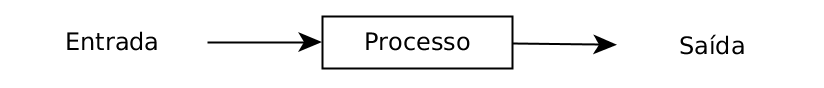
\includegraphics[width=0.7\textwidth]{./04-figuras/fund_teorica/process}
    \fonte{Adaptado de \citeonline[p.~2]{Dorf2011}}
    \label{fig:process}
\end{figure}

O controle de um processo pode assumir duas formas distintas: malha aberta ou malha fechada, sendo que um sistema de controle em malha aberta é composto, além do processo, por um controlador e um atuador para se obter a resposta desejada sem o uso de realimentação \cite[p.~2]{Dorf2011}. Um exemplo de sistema deste tipo é mostrado na Figura \ref{fig:open_loop_control_system}.

\begin{figure}[!htb]
    \centering
    \caption{Diagrama representando um sistema de controle em malha aberta}
    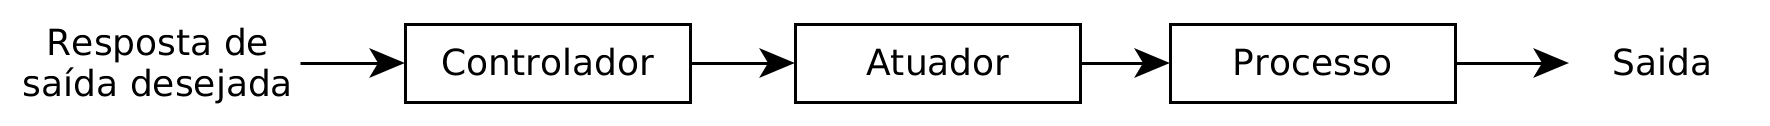
\includegraphics[width=0.95\textwidth]{./04-figuras/fund_teorica/open_loop_control_system}
    \fonte{Adaptado de \citeonline[p.~2]{Dorf2011}}
    \label{fig:open_loop_control_system}
\end{figure}

Em oposição a um sistema de controle em malha aberta, um em malha fechada incorpora, além dos componentes que aquele inclui, uma medição dos estados atuais para serem comparados com os valores desejados para o processo. Um exemplo de um sistema de controle em malha fechada simples é mostrado na Figura \ref{fig:closed_loop_control_system}. Os sistemas em malha fechada apresentam várias vantagens sobre os em malha aberta como, por exemplo, a capacidade de rejeitar distúrbios externos e melhorar a atenuação de ruídos nas medições, elementos estes que são inevitáveis em aplicações no mundo real \cite[p.~3]{Dorf2011}.

\begin{figure}[!htb]
    \centering
    \caption{Diagrama representando um sistema de controle em malha fechada}
    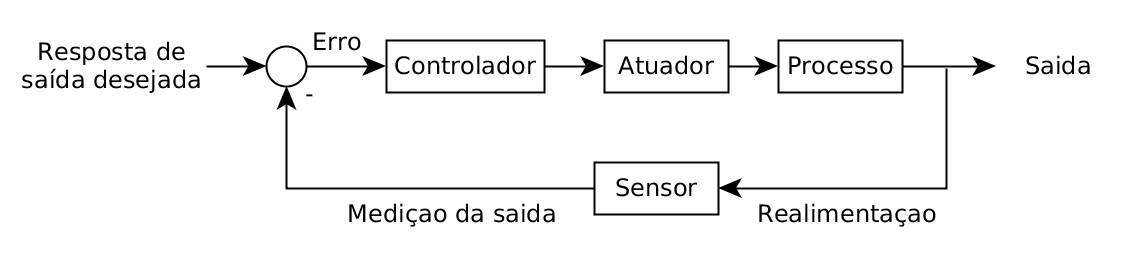
\includegraphics[width=0.95\textwidth]{./04-figuras/fund_teorica/closed_loop_control_system}
    \fonte{Adaptado de \citeonline[p.~3]{Dorf2011}}
    \label{fig:closed_loop_control_system}
\end{figure}

Como já foi visto, um processo representa a relação entre a entrada e a saída de um sistema sendo que há diferentes formas de fazê-lo. Uma forma de representar sistemas contínuos e é utilizando o espaço de estados.

%\subsection{Funções de Transferência}
%\label{subsec:fundamentacaoTeorica-tfs}
%%Ogata 15 do pdf; Dorf 65 do pdf
A função de transferência de um sistema representa a relação que descreve as dinâmicas do sistema em questão e é definida pela razão entre as transformadas de Laplace das variáveis de saída e de entrada com todas as condições iniciadas definidas como zero \cite[p.~65]{Dorf2011}. A forma de uma função de transferência é dada a seguir:
\begin{center}
$G(s) = \frac{Y(s)}{X(s)}$
\end{center}
em que $G(s)$ é a função de transferência que descreve o sistema, $Y(s)$ é a transformada de Laplace da variável de saída do sistema e $X(s)$ é a transformada de Laplace da variável de entrada, ambas considerando as condições iniciais definidas como zero.

Apesar de ser amplamente utilizada, o uso de funções de transferência tem certas limitações. As transformadas de Laplace só podem ser utilizadas sobre sistemas descritos por equações e diferencias lineares e sem parâmetros variantes no tempo e, portanto, o uso das funções de transferência se restringem aos casos em que estas condições são satisfeitas.

Além da representação a partir de funções de transferência, uma forma alternativa de representar as dinâmicas do sistema é a representação no espaço de estados.



\subsection{Espaço de Estados}
\label{subsec:fundamentacaoTeorica-ss}

%Ogata 29 do pdf (digrma de blocos na pag 32); Dorf 165 do pdf
A representação de um sistema dinâmico no espaço de estados descreve um sistema a partir das seguintes equações :
\begin{center}\label{eq:k1}
%$\dot{x}(t)=A(t)x(t)+B(t)u(t)$ \\
%$y(t)=C(t)x(t)+D(t)u(t)$
$\dot{x}=Ax+Bu$ \\
$y=Cx+Du$
\end{center}
%em que $A(t)$ é a matriz de estados, $B(t)$ a matriz de entrada, $C(t)$ a matriz de saída, $D(t)$ a matriz de transmissão direta, $x$ é o vetor de variáveis de estado, $u$ o vetor de entradas e $y$ o vetor de saídas. A Figura \ref{fig:ss_diagram} exibe um diagrama de blocos para a representação em espaço de estados definida.
em que $A$ é a matriz de estados, $B$ a matriz de entrada, $C$ a matriz de saída, $D$ a matriz de transmissão direta, $x$ é o vetor de variáveis de estado, $u$ o vetor de entradas e $y$ o vetor de saídas. A Figura \ref{fig:ss_diagram} exibe um diagrama de blocos para a representação em espaço de estados definida.

\begin{figure}[!htb]
    \centering
    \caption{Diagrama de blocos de um sistema linear e contínuo tempo representado no espaço de estados}
    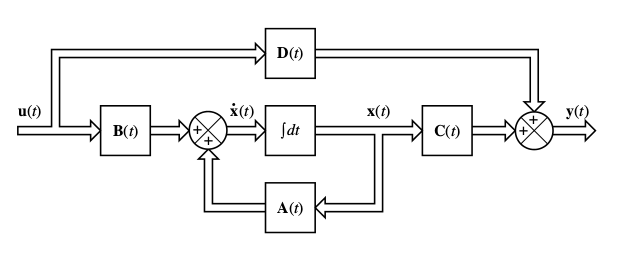
\includegraphics[width=0.9\textwidth]{./04-figuras/fund_teorica/ss_diagram}
    \fonte{\citeonline[p.~32]{Ogata2010}}
    \label{fig:ss_diagram}
\end{figure}

A representação no espaço de estados oferece uma ferramenta poderosa para a manipulação da representação do sistema, permitindo que as variáveis de estado sejam representadas de forma independente entre si a partir do processo de desacoplamento delas.

O processo de desacoplamento de variáveis de estado é baseado em ferramentas matemáticas aplicando manipulações sobre frações parciais. A partir deste processo, por exemplo, o sistema mostrado na Figura \ref{fig:ss_coupled}, que representa um sistema de controle de um motor CC com velocidade como saída e é representado pela função de transferência:
\begin{equation}
G(s)=\frac{30(s+1)}{(s+5)(s+2)(s+3)}
\end{equation}
pode ser representado por uma função de transferência do tipo:
\begin{equation}
G(s)=\frac{q(s)}{(s-s_1)(s-s_2)(s-s_3)}
\end{equation}
cuja resposta é ditada por $s_1$, $s_2$ e $s_3$. Utilizando a expansão de frações parciais, pode-se representar a mesma função de transferência por \cite[p.~183]{Dorf2011}:
\begin{equation}
T(s)=\frac{k_1}{s+5}+\frac{k_2}{s+2}+\frac{k_3}{s+3}
\end{equation}

\begin{figure}[!htb]
    \centering
    \caption{Diagrama de blocos representando o controle de um motor CC com velocidade como saída}
    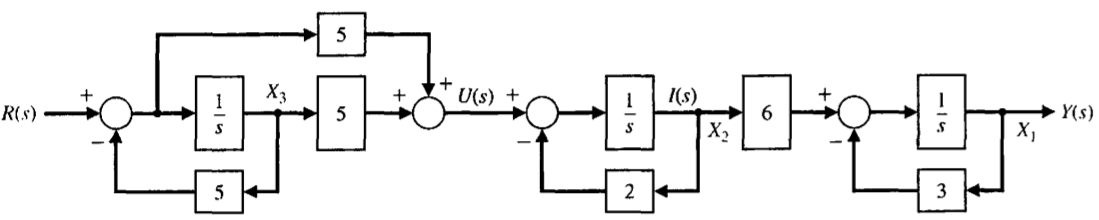
\includegraphics[width=1\textwidth]{./04-figuras/fund_teorica/ss_coupled_blocks}
    \fonte{\citeonline[p.~182]{Dorf2011}}
    \label{fig:ss_coupled}
\end{figure}

A partir de manipulações matemáticas relacionadas à expansão de frações parciais, constata-se que $k_1=-20$, $k_2=-10$ e $k_3=30$ \cite[p.~182]{Dorf2011}. Com isto, o sistema exibido na Figura \ref{fig:ss_coupled} pode ser representado como mostrado na Figura \ref{fig:ss_decoupled} que, como se pode ver, trata $X_1$, $X_2$ e $X_3$ de forma completamente independente e somando suas respectivas contribuições em $Y(s)$. Desta forma, pode-se ver claramente como cada variável de estado contribui para a saída ($Y(s)$) a partir de uma dada entrada ($X(s)$).

\begin{figure}[!htb]
    \centering
    \caption{Diagrama de blocos representando o controle de um motor CC com velocidade como saída e implementando desacoplamento das variáveis de estado}
    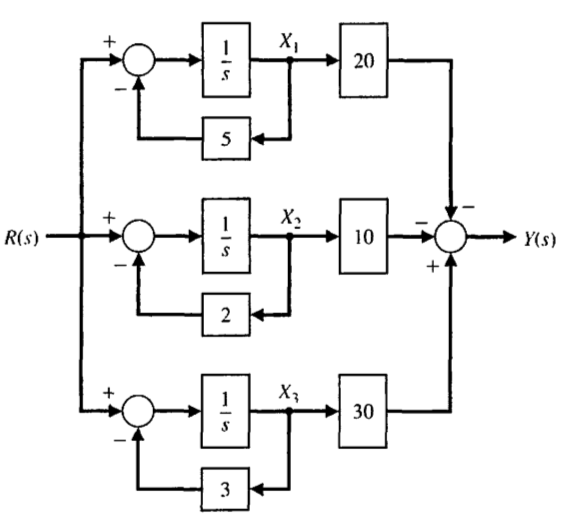
\includegraphics[width=0.6\textwidth]{./04-figuras/fund_teorica/ss_decoupled_blocks}
    \fonte{\citeonline[p.~182]{Dorf2011}}
    \label{fig:ss_decoupled}
\end{figure}










%No contexto deste trabalho, utilizou-se um sistema de controle em malha fechada no qual o processo a ser controlado diz respeito a um quadrotor. Além disto, os controladores utilizados foram de tipos bastante específicos: fuzzy e neuro-fuzzy, temas que são tratados nas próximas seções.

%Desacoplamento: Dorf pag 182 do pdf


\section{Redes Neurais Artificiais}
\label{sec:fundamentacaoTeorica-rna}
%redes neurais - pag 197 de jang
%adaptive networks - pag 199

%o que são redes neurais
Redes Neurais Artificiais (RNAs) são modelos computacionais bioinspirados no sistema neurológico humano. A motivação para o desenvolvimento e uso destes modelos é a grande complexidade do cérebro humano, definido por \citeonline{Haykin1998} como um computador altamente complexo, não linear e paralelo. O autor ainda define uma RNA como``\textit{a machine that is designed to} model \textit{the way in which the brain performs a particular task or function of interest}''\footnote{``uma máquina que é desenvolvida para \textit{modelar} a forma como o cérebro desempenha uma tarefa específica ou função de interesse'' (tradução nossa).}. Seguindo o modelo biológico do cérebro humano, uma RNA é composta por neurônios artificiais e pelas interações existentes entre estes neurônios: as sinapses.

%Explicação simplificada do sistema nervoso
A \autoref{fig:brainsistem} ilustra, em um diagrama de blocos, o sistema nervoso como um sistema de três estágios. A Rede Neural representa o cérebro em si, que recebe informações continuamente, as percebe e toma as decisões apropriadas para cada uma delas \cite[p.~24]{Haykin1998}.

\begin{figure}[!htb]
    \centering
    \caption{Representação em digrama de blocos do sistema nervoso}
    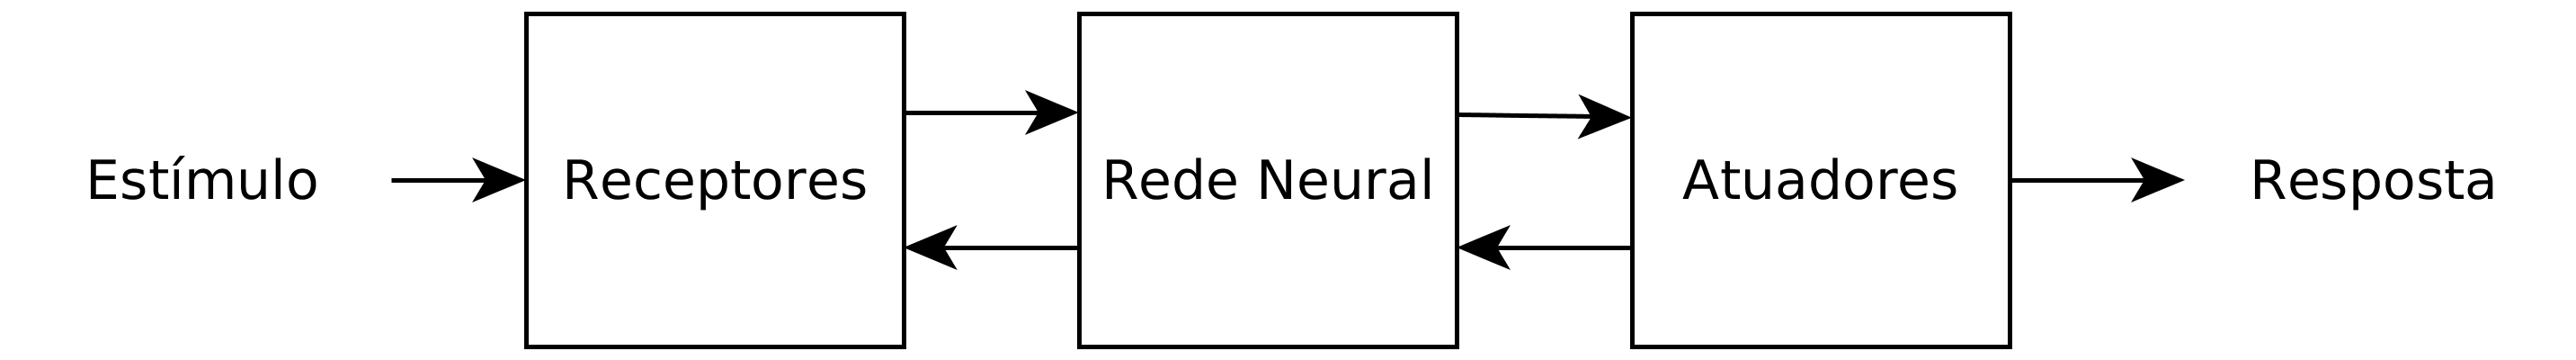
\includegraphics[width=0.9\textwidth]{./04-figuras/brain_sistem_block_diagram}
    \fonte{Adaptado de \citeonline[p.~28]{Haykin1998}}
    \label{fig:brainsistem}
\end{figure}

%O que são sinapses
Toda esta comunicação se dá a partir de sinapses, que são unidades estruturais e funcionais que mediam a interação entre neurônios. Seu funcionamento simplificado é o seguinte: o processo pré-sináptico libera uma substância transmissora que é difundida através da junção sináptica entre neurônios e então age sobre o processo pós-sináptico. Então, a sinapse converte o sinal elétrico pré-sinápitico em um sinal químico e, por fim, de volta a um sinal elétrico pós-sináptico \cite[p.~28]{Haykin1998}. É por meio deste processo de comunicação entre neurônios que adquirimos novos conhecimentos e relacionamos estímulos a respostas. É também devido a ele que podemos fazer associações diversas com acontecimentos no passado, evento que chamamos de \textit{memória}. O imenso poder que os neurônios possuem inspirou modelagens computacionais capazes de atuar em situações em que se deseja obter respostas adequadas a diferentes estímulos, e em outras relacionadas à memória e aprendizado. Um modelo neural comumente aplicado na literatura em problemas relacionados às RNAs é o perceptron. 

Um perceptron é um modelo computacional de um neurônio não linear e é ilustrado na Figura \ref{fig:neuronmodel}, em que $y_k$ é a saída do sistema obtido após o processamento neural relacionado às entradas $x_i$, cada qual contribuindo com um peso $w_{ki}$ para a junção de soma representada pelo bloco $\sum$. O processamento neural envolve ainda a função de ativação $\phi$ que, de acordo com o valor obtido na junção de soma, define o valor da saída $y_k$. Se o valor $v_k$ for maior que um limiar pré-determinado, a saída do sistema é ativada e terá o valor 1, caso contrário assumirá o valor 0, simulando assim o processo de transmissão ou não de impulsos elétricos que ocorrem nos neurônios biológicos.

\begin{figure}[!htb]
    \centering
    \caption{Modelo não linear de um neurônio}
    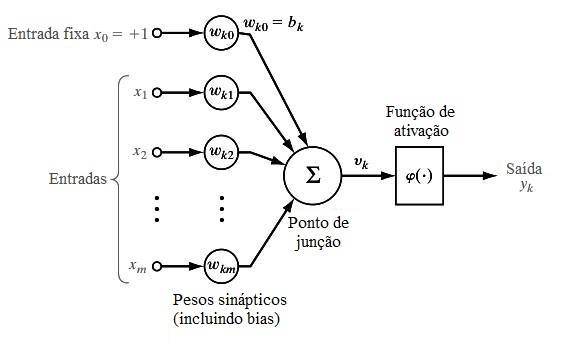
\includegraphics[width=0.8\textwidth]{./04-figuras/neuron-diagram-gray_traduzido}
    \fonte{Adaptado de \citeonline[p.~33]{Haykin1998}}
    \label{fig:neuronmodel}
\end{figure}

O modelo simples de um neurônio representado por perceptrons permite a simulação das já definidas sinapses, possibilitando a criação de RNAs complexas formadas por múltiplos neurônios, organizados em cadeias, como é mostrado na Figura \ref{fig:rna}. Neste exemplo, $x_1$, $x_2$ e $x_3$ são as entradas do sistema; os blocos 4, 5 e 6 representam, cada qual, um neurônio numa camada escondida; os blocos 7 e 8 representam os dois neurônios que compõem a camada de saída; e, por fim, $x_7$ e $x_8$ são as saídas de RNA. Redes como essa, que possuem mais de uma camada de neurônios, são denominadas \textit{Multilayer Perceptron} (MLP\footnote{Perceptron Multicamada (tradução nossa).}). As diferentes combinações que se podem obter distribuindo os neurônios de uma RNA de diferentes maneiras fazem com que estas redes possam ser utilizadas em aplicações diversas relacionadas à IA e IC.

\begin{figure}[!htb]
    \centering
    \caption{Modelo de um \textit{MLP}}
    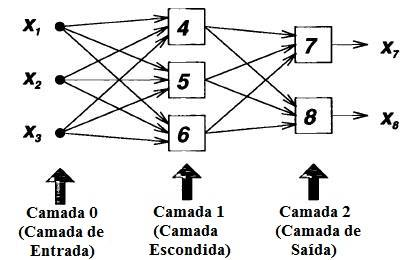
\includegraphics[width=0.6\textwidth]{./04-figuras/fund_teorica/rna_traduzido}
    \fonte{Adaptado de \citeonline[p.~205]{Jang1997}}
    \label{fig:rna}
\end{figure}

%vantagens das RNAs/ Funcionamento das RNAs
A principal característica de uma rede neural artificial que a torna interessante para aplicações computacionais é a sua capacidade de aprendizado. O procedimento usado para efetuar o processo de aprendizado é chamado \textit{algoritmo de aprendizado}, cuja função é modificar os pesos sinápticos da rede de forma ordenada para atingir um objetivo desejado \cite[p.~24]{Haykin1998}. É a partir deste aprendizado que as RNAs alcançam uma ótima taxa de generalização, fazendo delas fortes aliadas, por exemplo, para reconhecimento de padrões. Controladores que utilizam técnicas relacionadas a RNAs se beneficiam justamente destas capacidades de aprendizado e generalização conferidas por elas.

O controlador desenvolvido neste trabalho utiliza RNAs com treinamento supervisionado, que são treinadas a partir de um conjunto de entradas mapeadas no valor de suas respectivas saídas, resultando na obtenção de um conjunto de retas com parâmetros ajustados de acordo com os dados do treinamento. São as retas obtidas após este treinamento que conferem à rede o poder de generalização, permitindo que novas entradas sejam mapeadas para saídas que condizem com o cenário em questão.

Além disto, como o controlador projetado é do tipo Neuro-\textit{Fuzzy}, as retas ajustadas após o treinamento se enquadram num grupo especial correspondendo cada qual a uma função de pertinência de conjuntos \textit{Fuzzy}, assunto este que é abordado na seção seguinte.


\section{Lógica Fuzzy}
\label{sec:fundamentacaoTeorica-fuzzy}
%teoria de conjuntos fuzzy - pag 13 de jang
%inferencia fuzzy e raciocinio fuzzy - pag 47 jang

A lógica \textit{fuzzy} é uma alternativa à lógica convencional\footnote{lógica aristotélica.}, que permite uma abordagem diferente relacionada à pertinência de elementos a conjuntos implementando a possibilidade de se obter uma pertinência parcial para a definição desses conjuntos. A principal aplicação da lógica \textit{fuzzy} são os sistemas de inferência \textit{fuzzy}, tema que será abordado na Seção \ref{sec:sistema_inferencai_fuzzy}. As Seções \ref{sec:cojuntos_fuzzy}, \ref{sec:regras_fuzzy} e \ref{sec:raciocinio_fuzzy} referentes a conjuntos, regras e raciocínio \textit{fuzzy} respectivamente tratam dos diferentes componentes utilizados nestes sistemas. 
%e fazendo ainda uso de variáveis e termos linguísticos 

\subsection{Conjuntos \textit{Fuzzy}}
\label{sec:cojuntos_fuzzy}

Os conjunto \textit{fuzzy} são os componentes elementares dos sistema de inferência \textit{fuzzy} e se contrapõem àqueles definidos pela lógica tradicional, que restringe, aos valores 0 e 1, o grau de pertinência $\mu$ de um elemento $u$ a um conjunto $A$. Na lógica tradicional, este grau é definido da seguinte forma:
\begin{align*}
&\mu_A(u) = 1, \mbox{ se } u \mbox{ é um elemento do conjunto } A, \mbox{ e }\\
&\mu_A(u) = 0, \mbox{ se } u \mbox{ não é um elemento do conjunto } A
\end{align*}

Com isto, ou um elemento pertence a um conjunto ou não. Já os conjuntos \textit{fuzzy} permitem um grau de flexibilidade acerca do grau pertinência de cada elemento ao conjunto, sendo este grau definido por uma \textit{função de pertinência}. A definição formal de conjuntos \textit{fuzzy} e funções de pertinência é dada por \citeonline[p.~14]{Jang1997} como:
\begin{align*}
	A = \{(x,\mu_A(x)) \vert x \in X\}
\end{align*}

Nesta definição, um conjunto \textit{fuzzy} $A$ é composto pelos pares $(x,\mu_A(x))$ de cada elemento $x$ pertencente a um conjunto $X$, em que $x$ é o elemento em si e $\mu_A(x)$ é o grau de pertinência de $x$ ao conjunto $A$, que pode assumir qualquer valor entre 0 e 1, em que 0 representa a não-pertinência total do elemento ao conjunto e 1 representa a pertinência total a ele.

Como se pode perceber, a definição de um conjunto \textit{fuzzy} é uma simples extensão da referente a um conjunto clássico, no qual a função de pertinência (ou função característica) apenas pode assumir os valores 0 e 1. Se uma função de pertinência $\mu_A(x)$ de um conjunto \textit{fuzzy} $A$ é restrita a assumir os valores 0 ou 1, então ele é reduzido a um conjunto clássico \cite[p.~14]{Jang1997}.

Para melhor exemplificar a definição de conjuntos \textit{fuzzy}, tome como exemplo a Figura \ref{fig:fuzzy_sets_jang}. Neste caso, a variável idade (\textit{age}) é dividida em três subconjuntos \textit{fuzzy}, \textit{young, middle aged} e \textit{old}\footnote{jovem, meia idade e velho, respectivamente (tradução nossa).}, representados pelas funções de pertinência que os descrevem. Cada idade não precisa possuir necessariamente grau de pertinência 1 para algum conjunto e pode ainda pertencer simultaneamente a mais de um. A idade 30, por exemplo pertence ao conjunto jovem com grau de pertinência de 0,5 e também pertence ao conjunto meia idade com o mesmo grau.

\begin{figure}[!htb]
    \centering
    \caption{Funções de pertinência representando três conjuntos \textit{fuzzy} para a variável idade}
    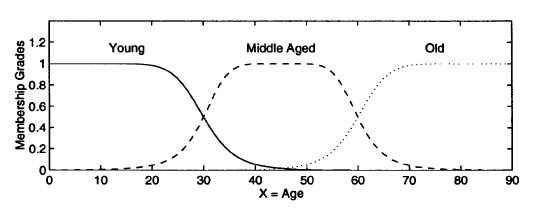
\includegraphics[width=0.8\textwidth]{./04-figuras/fund_teorica/fuzzy_sets_jang}
    \fonte{\citeonline[p.~17]{Jang1997}}
    \label{fig:fuzzy_sets_jang}
\end{figure}

Além dos conjuntos \textit{fuzzy}, há outro aspecto fundamental para o funcionamento desta lógica alternativa e poderosa: as regras \textit{fuzzy}.

%--revisao--
\subsection{Regras \textit{Fuzzy}}
\label{sec:regras_fuzzy}

As regras \textit{fuzzy} são os componentes de um sistema de inferência \textit{fuzzy} responsáveis por definir as relações entre as entradas do sistema e suas saídas e assumem a forma
\begin{center}
se $x$ é $A$ então $y$ é $B$
\end{center}
sendo ``$x$ é $A$'' denominada premissa  e ``$y$ é $B$'', consequente da regra em que $x$ e $y$ são \textit{variáveis linguísticas} de entrada e saída respectivamente  e $A$ e $B$ são os valores que elas assumem, representados por \textit{termos linguísticos}.

Uma variável linguística, segundo \citeonline[p.~54]{Jang1997}, é caracterizada por uma quíntupla $(x,T(x),X,G,M)$ em que $x$ é o nome da variável; $T(x)$ é o conjunto de termos de $x$, que é o conjunto de seus valores linguísticos ou termos linguísticos; $X$ é o universo de discurso; $G$ é uma regra sintática que gera os termos em $T(x)$; e $M$ é uma regra semântica que associa a cada termo linguístico A seu respectivo $M(A)$, em que $M(A)$ denota um conjunto \textit{fuzzy} em $X$.

Para facilitar a compreensão das definições relacionadas às variáveis linguísticas, o seguinte exemplo foi dado \cite[p.~55]{Jang1997}: se \textit{idade} é interpretado como uma variável linguística, então seu conjunto de termos $T(idade)$ poderia ser dado por:
\begin{align*}
\mbox{\textit{T(idade) = }}\{ &\mbox{ \textit{novo, não-novo, muito novo, não muito-novo,}} \dots, \\
&\mbox{ \textit{meia-idade, não de meia-idade,}} \dots, \\
&\mbox{ \textit{velho, não-velho, muito velho, mais ou menos velho, não muito velho,}} \dots, \\
&\mbox{ \textit{não muito novo e não muito velho,}} \dots \},
\end{align*}

Em que cada termo em $T(idade)$ é caracterizado por um conjunto \textit{fuzzy} de um universo de discurso $X = [0,100]$, como mostrado na Figura \ref{fig:fuzzy_rules_jang}. Geralmente, se diz ``idade é jovem'' para denotar a atribuição do valor linguístico jovem à variável linguística idade. A regra sintática se refere à forma como os valores linguísticos no conjunto de termos $T(idade)$ são gerados. A regra semântica define a função de pertinência de cada valor linguístico do conjunto de termos. A Figura \ref{fig:fuzzy_rules_jang} mostra algumas das funções de pertinência típicas para a variável linguística idade.

\begin{figure}[!htb]
    \centering
    \caption{Exemplo de função de pertinência do conjunto de termos T(idade)}
    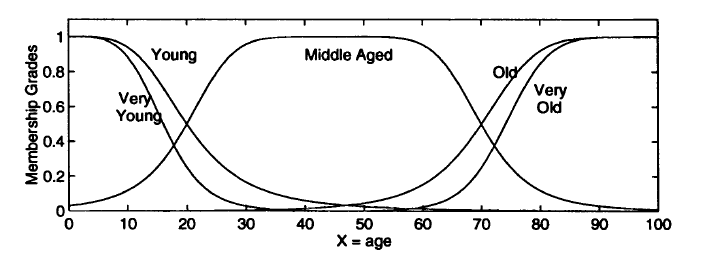
\includegraphics[width=0.8\textwidth]{./04-figuras/fund_teorica/fuzzy_rules_jang}
    \fonte{\citeonline[p.~55]{Jang1997}}
    \label{fig:fuzzy_rules_jang}
\end{figure}

Diversas regras \textit{fuzzy} fazem parte do nosso cotidiano. Exemplos possuindo a variável linguística \textit{idade} como variável linguística de entrada e saída respectivamente incluem:
\begin{center}
se \textit{idade} é \textit{jovem} então \textit{energia} é \textit{alta} \\
se \textit{sabedoria} é \textit{grande} então \textit{idade} é \textit{velha}
\end{center}

Um outro componente dos sistemas de inferência \textit{fuzzy} agrega muito valor ao uso de regras \textit{fuzzy}, permitindo a aplicação aproximada delas: o raciocínio \textit{fuzzy}.

\subsection{Raciocínio \textit{Fuzzy}}
\label{sec:raciocinio_fuzzy}

O processo de raciocínio \textit{fuzzy}, também conhecido como raciocínio aproximado, é um procedimento de inferência que deriva conclusões de um conjunto de regras \textit{fuzzy} \textit{se-então} como fatos conhecidos \cite[p.~62]{Jang1997} e é a partir dele que se pode fazer uma generalização a partir da regra básica na lógica tradicional com duas variáveis, denominada \textit{modus ponens}.

De acordo com a regra \textit{modus ponens}, podemos inferir a verdade da proposição $B$ a partir da verdade de $A$ e a implicação $A \rightarrow B$ (se A então B). Por exemplo, se $A$ é identifica por ``o tomate é vermelho'' e $B$ por ``o tomate está maduro'', então se é verdade que ``o tomate é vermelho'', é também verdade que ``o tomate está maduro''.

Contudo, o raciocínio humano emprega constantemente o modus ponens em uma maneira aproximada. Por exemplo, usando a mesma regra de implicação ``se o tomate é vermelho, então ele está maduro'', e sabemos que o ``o tomate está mais ou menos vermelho'' ($A^\prime$), então podemos inferir que ``o tomate está mais ou menos maduro'' ($B^\prime$), em que $A^\prime$ é próximo de $A$ e $B^\prime$ é próximo de $B$. Quando $A$, $B$, $A^\prime$ e $B^\prime$ são conjuntos \textit{fuzzy} do universo adequado, o procedimento de inferência descrito é chamado raciocínio aproximado ou raciocínio \textit{fuzzy}, podendo ser também chamado \textit{modus ponens} generalizado (GMP\footnote{Do inglês, \textit{Generalized Modus Ponens}}) \cite[p.~65]{Jang1997}.

A definição formal do raciocínio aproximado (raciocínio \textit{fuzzy}) é dada por \citeonline[p.~65]{Jang1997} como: sejam $A$, $A^\prime$, e $B$ conjuntos \textit{fuzzy} de $X$, $X$ e $Y$ respectivamente; assuma que a implicação \textit{fuzzy} $A \rightarrow B$ é expressa como uma relação $R$ em $X \times Y$. Então, o conjunto \textit{fuzzy} B induzido por ``$x$ é $A$'' e a regra \textit{fuzzy} ``se $x$ é $A$ então $y$ é $B$'' é definida por:
\begin{align*}
\mu_{B^\prime}(y) &= \max\nolimits_x \min[\mu_{A^\prime}, \mu_R(x,y)]
\\
&= \vee_x[\mu_{A^\prime}(x) \wedge \mu_R(x,y)], \\
\mbox{ou, equivalentemente,} \\
B^\prime &= A^\prime \circ R = A^\prime \circ (A \rightarrow B).
\end{align*}
 
Assim, podemos usar o procedimento de inferência do raciocínio \textit{fuzzy} para derivar conclusões, dado que a implicação \textit{fuzzy} $A \rightarrow B$ é definida como uma relação \textit{fuzzy} binária apropriada.

Uma vez definidos os conjuntos, regras e raciocínio \textit{fuzzy}, pode-se mostrar como eles são utilizados em conjunto pelos sistemas de inferência \textit{fuzzy}.
 
\subsection{Sistema de Inferência Fuzzy}
\label{sec:sistema_inferencai_fuzzy}

Um sistema de inferência fuzzy (FIS, do nome em inglês \textit{Fuzzy Inference System}) é uma ferramenta computacional popular e poderosa baseada nos conceitos de teoria de conjuntos fuzzy, regras fuzzy e raciocínio fuzzy. Há uma grande variedade de aplicações para sistemas de inferências fuzzy tais como controle automatizado, classificação de dados, análise de decisão, sistemas especialistas, predição de séries temporais, robótica e reconhecimento de padrões \cite[p.~73]{Jang1997}.

A estrutura básica de um FIS consiste de três componentes conceituais: uma base de regras, que contém uma seleção de regras fuzzy; um dicionário (ou base de dados), que define as funções de pertinência usadas nas regras fuzzy; e o mecanismo de raciocínio, que realiza o procedimento de inferência (geralmente o raciocínio fuzzy) sobre as regras e fatos dados para obter uma saída ou conclusão razoável \cite[p.~73]{Jang1997}. Sistemas de inferência fuzzy diferentes implementam estruturas ligeiramente diferentes entre si, havendo entretanto, três tipos principais de sistemas que podem ser aplicados aos mais diversos casos.

% corte 01
Os três principais tipos de FIS são os Mamdani, Tsukamoto e Sugeno e a diferença entre eles reside basicamente no consequente de suas regras fuzzy \cite[p.~74]{Jang1997}.

No sistema de inferência fuzzy Mamdani, o consequente das regras \textit{se-então} são conjuntos fuzzy. Desta forma, um sistema de inferências fuzzy Mamdani possui regras do seguinte tipo para um sistema com duas entradas e uma saída:
\begin{center}
se $x$ é $A$ e $y$ é $B$, então $z$ é $C$
\end{center}

Em que $x$, $y$ e $z$ são variáveis linguísticas nos universos de discurso $X$, $Y$ e $Z$, respectivamente e $A$, $B$ e $C$ são valores (termos) linguísticos. Com isto, um exemplo de sistema de inferências fuzzy Mamdani é formado pelas seguintes regras fuzzy:
\begin{align*}
\begin{cases}
&\mbox{Se }X  \mbox{é pequeno e } Y \mbox{é pequeno então } Z \mbox{ é muito negativo} \\
&\mbox{Se }X  \mbox{é pequeno e } Y \mbox{é grande então } Z \mbox{ é pouco negativo} \\
&\mbox{Se }X  \mbox{é grande e } Y \mbox{é pequeno então } Z \mbox{ é pouco positivo} \\
&\mbox{Se }X  \mbox{é grande e } Y \mbox{é grande então } Z \mbox{ é muito positivo} 
\end{cases}
\end{align*}

No caso do sistema de inferência fuzzy Tsukamoto, o consequente de cada regra fuzzy \textit{se-então} é representada por um conjunto fuzzy com uma função de pertinência monotônica\footnote{Uma função sempre crescente ou sempre decresente; uma função cuja derivada nunca muda de sinal}. Um exemplo de modelo fuzzy Tsukamoto de entrada única pode ser expressa como:
\begin{align*}
\begin{cases}
&\mbox{Se }X  \mbox{é pequeno então } Y \mbox{ é } C_1\\
&\mbox{Se }X  \mbox{é médio então } Y \mbox{ é } C_2\\
&\mbox{Se }X  \mbox{é grande então } Y \mbox{ é } C_3
\end{cases}
\end{align*}

No sistema de inferência fuzzy Sugeno, também conhecido como TSK (Takagi-Sugeno-Kang), o consequente é um função envolvendo as variáveis de entrada. Com isto, uma regra fuzzy típica de um modelo fuzzy Sugeno possui a seguinte forma:
\begin{center}
se $x$ é $A$ e $y$ é $B$, então $z = f(x,y)$,
\end{center}

Em que $A$ e $B$ são conjuntos fuzzy do antecedente, enquanto $z = f(x,y)$ é uma função no consequente. Geralmente, $f(x,y)$ é uma função polinomial sobre as variáveis $x$ e $y$, mas pode ser qualquer função, contanto que seja capaz de descrever apropriadamente a saída do modelo dentro da região fuzzy especificada pelo antecedente da regra. Um exemplo de sistema de inferências fuzzy TSK com duas entradas e uma saída é formado pelas seguintes regras fuzzy:
\begin{align*}
\begin{cases}
&\mbox{Se }X  \mbox{é pequeno e } Y \mbox{é pequeno então } z=-x+y+1 \\
&\mbox{Se }X  \mbox{é pequeno e } Y \mbox{é grande então } z=-y+3  \\
&\mbox{Se }X  \mbox{é grande e } Y \mbox{é pequeno então } z=-x+3  \\
&\mbox{Se }X  \mbox{é grande e } Y \mbox{é grande então } z=x+y+2  
\end{cases}
\end{align*}

Esta propriedade dos sistemas de inferência fuzzy Sugeno de possuírem, como consequente, funções paramétricas que relacionam as premissas abre várias possibilidades para sua aplicação. Uma delas é implementada por uma técnica que alia o poder das RNAs ao do FIS: o sistema de inferência neuro-fuzzy.

%Esta propriedade dos sistemas de inferência fuzzy Sugeno de possuírem, como consequente, uma função que relaciona as premissas abre várias possibilidades para sua aplicação. Uma delas é implementada por uma técnica que alia o poder de aprendizado e generalização das RNAs ao uso de variáveis linguísticas, definições de pertinência parciais e raciocínios aproximados da lógica fuzzy: o sistema de inferência neuro-fuzzy.

% corte 01
%Um sistema de inferência fuzzy pode tomar entradas fuzzy ou \textit{crisp}, mas as saídas que ele produz são sempre conjuntos fuzzy. Algumas vezes, é necessário se obter uma saída \textit{crisp}, principalmente quando o sistema de inferência fuzzy é usado como um controlador. Desta forma, se faz necessário um método de defuzzificação para extrair um valor \textit{crisp} que melhor represente um conjunto fuzzy.

%Com entradas e saídas \textit{crisp}, um sistema de inferência fuzzy implementa um mapeamento não linear do espaço de entrada para o espaço de saída. Este mapeamento é realizado por um número de regras fuzzy \textit{se-então}, cada qual descrevendo o comportamento local do mapeamento. Em particular, o antecedente de uma regra define a região fuzzy no espaço de entrada, enquanto o consequente especifica a saída na região fuzzy \cite[p.~73]{Jang1997}.

%\section{\textit{Soft Computing} e Neuro-Fuzzy}
\section{Redes Neuro-Fuzzy}
\label{sec:fundamentacaoTeorica-neuro-fuzzy}
%Página 1 (introdução); Página 333 (Neuro-Fuzzy Modeling) de Jang1997
%
%De Jang1997, incluir mais texto
%	Fuzzy: Mamdani, Sugeno, TSK
%	RNA: Aprendizado supervisionado x não-supervisionado; aprendizado por reinforcement

Aliando o poder das RNAs, que reconhecem padrões e se adaptam para lidar com mudanças no ambiente, aos sistemas de inferência \textit{fuzzy}, que incorporam o conhecimento humano e executam inferências e tomadas de decisão, surgiram os sistemas de inferência neuro-\textit{fuzzy} (ANFIS, acrônimo para \textit{Adaptive Neuro-Fuzzy Inference System}), uma nova ferramenta computacional poderosa amplamente utilizada em diversos contextos \cite[p.~1]{Jang1997}.

\subsection{ANFIS: \textit{Adaptive Neuro-Fuzzy Inference Systems}}
Segundo \citeonline[p.~335]{Jang1997}, do ponto de vista funcional, praticamente não há limitações para a gama de funções, no sentido matemático, de uma rede neuro-\textit{fuzzy}, exceto pela exigência de ela ser diferenciável por partes. Devido às mínimas restrições, redes neuro-\textit{fuzzy} podem ser empregadas diretamente em uma grande variedade de aplicações de modelagem, tomadas de decisão, processamento de sinal e controle.

%\subsubsection{Arquitetura ANFIS}
Para simplificar, a arquitetura ANFIS\footnote{Sistema de Inferência Neuro-\textit{Fuzzy} Adaptativo (tradução nossa).} será descrita considerando-a dotada de duas entradas $x$ e $y$ e uma saída $z$. Para um modelo \textit{fuzzy} Sugeno de primeira ordem, um conjunto comum de regras do tipo \textit{se-então} é o seguinte:

\begin{center}
    Regra 1: Se $x$ é $A_1$ e $y$ é $B_1$, então $f_1 = p_1x + q_1y + r_1$,\\
    Regra 2: Se $x$ é $A_2$ e $y$ é $B_2$, então $f_2 = p_2x + q_2y + r_2$. 
\end{center}

A Figura \ref{fig:anfis} ilustra um mecanismo de raciocínio para o modelo Sugeno e a arquitetura ANFIS equivalente, em que nós de uma mesma camada têm funções similares, como descrito a seguir.
\begin{figure}[!htb]
    \centering
    \caption{Equivalência entre modelo \textit{fuzzy} Sugeno e ANFIS; (a) Um modelo \textit{fuzzy} Sugeno com duas entradas de primeira ordem com duas regras; (b) arquitetura ANIFS equivalente}
    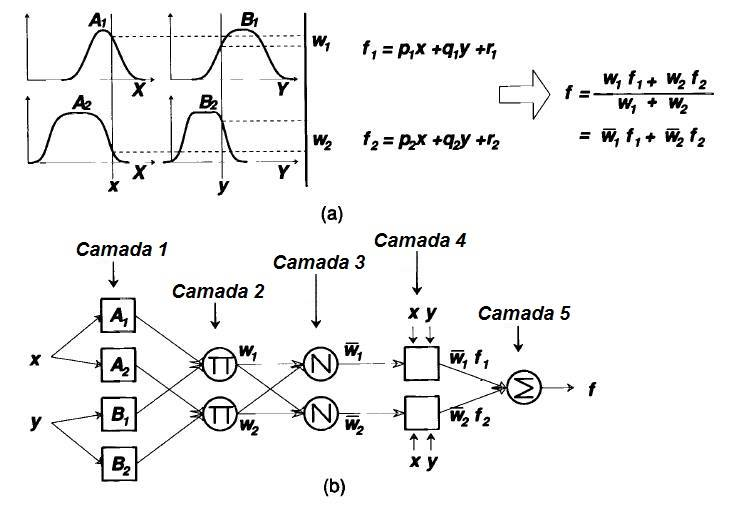
\includegraphics[width=0.8\textwidth]{./04-figuras/fund_teorica/anfis_traduzido}
    \fonte{\cite[p.~336]{Jang1997}}
    \label{fig:anfis}
\end{figure}

Na camada 1 (\textit{Layer 1}), todo nó \textit{i} é um nó adaptativo com uma função de nó do tipo:
\begin{align*}
    O_{1,i} = \mu_{A_{i}}(x), \mbox{ para } i = 1, 2, \mbox{ ou}\\
    O_{1,i} = \mu_{B_{i-2}}(y), \mbox{ para } i = 3, 4
\end{align*}
em que $x$ (ou $y$) é a entrada para o nó $i$ e $A_{i}$ (ou $B_{i-2}$) é um termo linguístico (como ``pequeno'' ou ``grande'') associado a este nó. Em outras palavras, $O_{1,i}$ é o grau de pertinência de um conjunto \textit{fuzzy} $A$ ($A_1$, $A_2$, $B_1$ ou $B_2$) e especifica o grau em que a entrada $x$ (ou $y$) satisfaz o quantificador $A$. Aqui, a função de pertinência $A$ pode ser qualquer função de pertinência parametrizada apropriada. Parâmetros nesta camada são chamados parâmetros de premissa \cite[p.~336]{Jang1997}.

Na camada 2 (\textit{Layer 2}), cada nó é um nó fixo rotulado $\prod$, cuja saída é o produto de todos sinais de entrada:
\begin{align*}
    O_{2,i} = w_i = \mu_{A_{i}}(x)\mu_{B_{i-2}}(y), i = 1, 2.
\end{align*}

Cada nó de saída representa a força de ativação de uma regra. Em geral, qualquer outro operador norma-T\footnote{Operador de interseção \cite[p.~337]{Jang1997}} que desempenhe a operação \textit{AND} \textit{fuzzy} pode ser usado como função de nó nesta camada \cite[p.~337]{Jang1997}.

Na camada 3 (\textit{Layer 3}), cada nó é um nó fixo rotulado N. O $i$-ésimo nó calcula a taxa da força de ativação da $i$-ésima regra pela soma da força de ativação de todas as regras:
\begin{align*}
    O_{3,i} = \bar{w_i} = \frac{w_i}{w_1 + w_2}, i = 1, 2.
\end{align*}

Por conveniência, saídas desta camada são chamadas forças de ativação normalizadas \cite[p.~336]{Jang1997}.

Na camada 4 (\textit{Layer 4}), todo nó $i$ é um nó adaptativo com uma função nodal
\begin{align*}
    O_{4,i} = \bar{w_i}f_i = \bar{w_i}(p_ix+q_iy+r_i),
\end{align*}
em que $\bar{w_i}$ é um taxa da força de ativação normalizada da camada 3 e \{$p_i, q_i, r_i$\} é o conjunto de parâmetros deste nó. Parâmetros nesta camada são denominados parâmetros consequentes \cite[p.~336]{Jang1997}.

O único nó na camada 5 (\textit{Layer 5}) é um nó fixo denominado $\sum$, e é responsável por computar a saída global como a soma ponderada de todos os sinais de entrada:
\begin{align*}
    \mbox{saída global} = O_{5,i} = \sum_{i} {\bar{w_i}f_i} = \frac{\sum_{i} {w_if_i}}{\sum_{i} {w_i}} %\overline{w_i}(p_ix+q_iy+r_i),
\end{align*}

Com esta arquitetura, constrói-se uma rede neuro-\textit{fuzzy} (ANFIS) que é funcionalmente equivalente a um modelo \textit{fuzzy} Sugeno \cite{Jang1997}. Com isto, sistemas de inferência neuro-\textit{fuzzy} podem operar, por exemplo, utilizando o treinamento supervisionado de uma RNA para ajustar o valor dos parâmetros das funções de resposta dos sistemas de inferência \textit{fuzzy} Sugeno para uma dada operação. Um exemplo de aplicação para este tipo de rede seria o controle de sistemas não lineares.

\subsection{Controladores \textit{Fuzzy} e Neuro-\textit{Fuzzy}}
%Página 451 (Neuro-Fuzzy Control) de Jang1997

Um controlador lógico fuzzy (FLC)\footnote{Do inglês, \textit{Fuzzy Logic Controller}.} é um sistema de inferência fuzzy projetado especificamente para atuar como controlador de um sistema que se deseja controlar. Este FIS portanto possui, como entradas, sinais provenientes do sistema e, como saídas, sinais de atuação sobre ele.

Com o avanço dos microprocessadores e hardware, tem se criado uma diversidade ainda maior de domínios para aplicação de controladores lógicos fuzzy, que vão de eletroeletrônicos à indústria automobilística. De fato, para sistemas complexos ou mal definidos que não são facilmente sujeitados a métodos de controle convencionais, os FLCs proveem uma alternativa viável, uma vez que eles podem capturar os aspectos qualitativos aproximados do raciocínio de um humano e o processo de tomada de decisão. De qualquer forma, sem a capacidade adaptativa, a performance de um FLC se baseia exclusivamente em dois fatores: a disponibilidade de humanos com expertise e as técnicas de aquisição de conhecimento para converter esta expertise humana nas apropriadas regras fuzzy \textit{se-então} e funções de pertinência. Estes dois fatores restringem substancialmente o domínio de aplicações dos FLCs \cite[p.~451]{Jang1997}.

Nesse contexto, o uso de controladores neuro-fuzzy passou a se mostrar muito interessante, tendo em vista que eles eliminam os dois fatores citados que restringem bastante o domínio de aplicações dos FLCs, uma vez que os sistemas ANFIS preenchem as lacunas deixadas pelos FIS, eliminando a necessidade de humanos com expertise sobre o sistema e encorporando técnicas de aquisição de conhecimento.

Com isto, podem-se identificar algumas propriedades particulares aos controladores ANFIS que os tornam ótimas opções para diversos casos \cite[p.~458]{Jang1997}:
\begin{enumerate}
  \item Habilidade de aprendizado;
  \item Operação paralela;
  \item Representação do conhecimento estruturado;
  \item Melhor integração com outros métodos de controle.
\end{enumerate}

Como comparativo, é importante salientar que uma RNA possui as propriedades 1 e 2, mas não as 3 e 4, que são devidas à contribuição dos sistemas de inferência fuzzy \cite[p.~458]{Jang1997}. Um ANFIS, por aliar as duas técnicas, possui todas essas propriedades.

Ainda segundo o autor, há diversas formas diferentes de se projetar controladores neuro-fuzzy. A maioria deles são não lineares. Assim sendo, uma análise rigorosa para sistemas de controle neuro-fuzzy é difícil e continua sendo uma área desafiadora para outras investigações. Por outro lado, um controlador neuro-fuzzy geralmente contém um grande número de parâmetros, o que o torna mais versátil do que um controlador linear ao lidar com características não lineares de plantas. Desta forma, controladores neuro-fuzzy quase sempre superam controladores puramente lineares se devidamente projetados.

%Por outro lado, investigações usando redes neurais em sistemas de controle automatizados não receberam muita atenção até que a regra de aprendizado com \textit{backpropagaion} fosse reformulada em 1986. Desde então, pesquisas de controle neural têm evoluído rapidamente e um grande número de métodos que o implementam tem sido proposto na literatura \cite[p.~451]{Jang1997}.

%\subsubsection{Sistemas de Controle Realimentados}
%A \autoref{fig:feedback-control-system-diagram} é um diagrama de blocos de um típico sistema de controle realimentado, em que a planta (ou processo) representa o sistema dinâmico a ser controlado e o controlador emprega uma estratégia de controle para alcançar um objetivo proposto.
%
%\begin{figure}[!htb]
%    \centering
%    \caption{Diagrama de blocos de um sistema de controle realimentado}
%    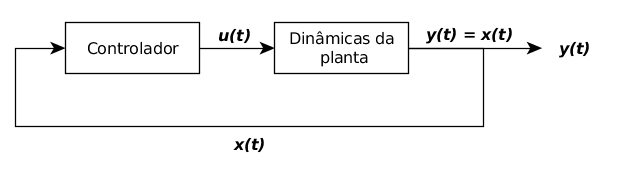
\includegraphics[width=0.9\textwidth]{./04-figuras/Jang1997_feedback_control_system_diagram}
%    \fonte{Adaptado de \citeonline[p.~455]{Jang1997}}
%    \label{fig:feedback-control-system-diagram}
%\end{figure}

%\subsubsection{Controlador Neuro-Fuzzy}
%Se o controlador da \autoref{fig:feedback-control-system-diagram} for substituído por RNAs ou sistemas de inferência fuzzy, obteríamos sistemas de controle neural ou fuzzy, respectivamente. Em outras palavras, métodos de controle neurais ou fuzzy são formas sistemáticas de construir redes neurais ou sistemas de inferência fuzzy como controladores com a intenção de se alcançar um objetivo de controle pré-estabelecido. Da mesma forma, um controle neuro-fuzzy se refere à concepção de métodos para controladores de lógica fuzzy que empregam técnicas de redes neurais. Em particular, podem-se citar métodos para ANFIS \cite[p.~458]{Jang1997}.





%\citeonline[p.~1]{Jang1997} define \textit{Soft Computing}\footnote{Computação Flexível, tradução nossa} (SC) como uma abordagem inovadora para construir sistemas inteligentes computacionais. Segundo ele, chegou-se a um momento em que soluções eficientes para problemas do mundo real requerem sistemas inteligentes que combinem conhecimento, técnicas e metodologias de diferentes fontes. Estes sistemas inteligentes deveriam possuir expertise humanóide com um domínio específico, se adaptar e aprender a agir melhor em mundanças de ambientes e explicar como eles tomam as decisões ou tomam ações.
%
%
%Os diferentes paradigmas que constituem a \textit{Soft Computing} incluem redes neurais, teoria de conjuntos fuzzy, métodos de otimização tais como algoritmos genéticos e \textit{simulated annealing}. Cada um destes métodos possui seu próprio ponto forte, como é mostrado no \autoref{qua:Jang1997_sc_constituents}. A integração adequada destas metodologias formam o núcleo da SC; a sinergia permite à SC a incorporar o conhecimento humano efetivamente, lidar com imprecisão e incerteza, e aprender para se adaptar a diferentes ou desconhecidos ambientes para melhor performance \cite[p.~2]{Jang1997}.
%
%\begin{quadro}[!htb]
    \centering
    \caption{Constituintes da \textit{Soft Computing} e inteligência artificial convencional\label{qua:Jang1997_sc_constituents}}
    \begin{tabular}{|c|c|}
        \hline
            \textbf{Medologia} & 
            \textbf{Ponto Forte} \\
        \hline
            Rede Neural &
            Aprendizado e Adaptção \\
        \hline
            \multirow{2}{*}{Teoria de Conjuntos Fuzzy}&Representação do conhecimento\\
            &via regras se-então\\
        \hline
            Algoritmos Genéticos e \textit{simulated annealing} &
            Pesquisa randômica sistemática \\

        % \hline
        %     \shortstack{Algoritmos Genéticos e \\ \textit{simulated annealing}} &
        %     Pesquisa randômica sistemática\\

        % \hline
        %     \multirow{2}{*}{\shortstack{Algoritmos Genéticos e \\ \textit{simulated annealing}}} &
        %     Pesquisa randômica sistemática\\

        \hline
            IA Convencional &
            Manipulação Simbólica \\
        \hline
    \end{tabular}
    \fonte{Adaptado de \citeonline[p.~2]{Jang1997}}
\end{quadro}


          % Fundamentação teórica
%    \chapter{Sistemas Não Lineares}
\label{chap:sistemas-nao-lineares}

Este trabalho consiste no projeto de um controlador para um quadrotor que, por se tratar de um sistema não linear intrinsecamente instável é comumente relacionado ao sistema de um pêndulo invertido, outro sistema do mesmo tipo mas com menor grau de complexidade. Desta forma, este capítulo trata, primeiramente e de forma mais superficial, do sistema do pêndulo invertido apenas para fazer uma introdução aos sistemas instáveis e, depois, faz uma introdução ao sistema de um quadrotor, que é o foco principal deste trabalho.

\section{Analogia ao Pêndulo Invertido}
\label{sec:sistemas-nao-lineares-pendulo}

Um sistema de pêndulo invertido consiste em uma haste suspensa verticalmente sobre um carro motorizado, como mostrado na Figura \ref{fig:diagrama-pendulo-invertido}. O objetivo do controle de atitude, que é referente ao controle de orientação angular, é manter a haste na posição vertical mesmo após o sistema sofrer alguma perturbação. Como o pêndulo invertido é um sistema instável, após sofrer esta perturbação a haste deverá cair a menos que uma ação de controle adequada seja exercida.

Neste exemplo, é considerado um problema bidimensional, em que o pêndulo se move apenas para a direita e para esquerda (i.e.\ no plano da página), mas não para frente e para trás (i.e\ no plano ortogonal a ela). Outra simplificação feita é a consideração de que o centro de gravidade da haste do pêndulo seja seu centro geométrico.

%\begin{figure}[!htb]
%    \centering
%    \caption{Diagrama do sistema de pêndulo invertido; (a) sistema de pêndulo invertido; (b) diagrama de corpo livre}
%    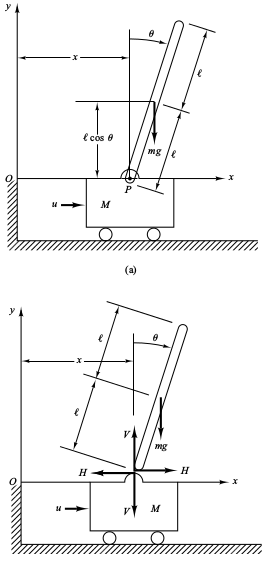
\includegraphics[width=0.55\textwidth]{./04-figuras/Ogata2010_inverted_pendulum_diagram_complete}
%    \fonte{\citeonline[p.~69]{Ogata2010}}
%    \label{fig:Ogata2010_inverted_pendulum_diagram_complete}
%\end{figure}
\begin{figure}[!htb]
    \centering
    \caption{Diagrama do sistema de pêndulo invertido}
    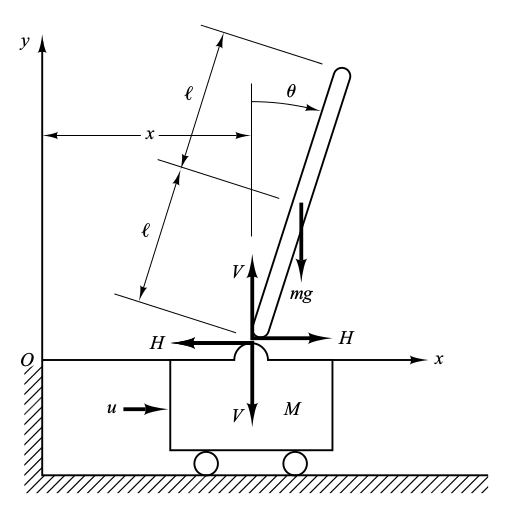
\includegraphics[width=0.6\textwidth]{./04-figuras/sistemas-nao-lineares/diagrama-pendulo-invertido}
    \fonte{Adaptado de \citeonline[p.~69]{Ogata2010}}
    \label{fig:diagrama-pendulo-invertido}
\end{figure}
%diagrama-pendulo-invertido

Além disso, o sistema mostrado na Figura \ref{fig:diagrama-pendulo-invertido}, assume que uma força $u$ seja aplicada ao carro, considerando $M$ como a massa do carro, $m$ a massa da haste, $g$ a força da gravidade, $x$ o deslocamento no eixo horizontal, $l$ a metade do comprimento da haste, $\theta$ o ângulo da haste com relação ao eixo vertical, $P$ o ponto de rotação do pêndulo sobre o carro, $H$ o movimento horizontal do centro de gravidade da haste do pêndulo e $V$ o movimento vertical do centro de gravidade da haste do pêndulo.

Com estes parâmetros, \citeonline[p.~69]{Ogata2010} mostra que o sistema descrito pode ser representado da seguinte maneira  no espaço de estados:
\begin{center}\label{eq:k1}
$\dot{x}=Ax+Bu$ \\
$y=Cx+Du$
\end{center}
em que:
%\begin{equation*}
%x=
%\left[ \begin{array}{@{}*{4}{c}@{}}
%     \theta & \dot{\theta} & x & \dot{x} \\
%\end{array} \right]^T
%\end{equation*}
%
%Além disto, o vetor $y$ de saída do sistema foi definido como:
\[
%	x =
%	\begin{bmatrix}
%	\theta & \dot{\theta} & x & \dot{x}
%	\end{bmatrix}^T\quad
	x =
		\begin{bmatrix}
		\theta \\ \dot{\theta} \\ x \\ \dot{x}
		\end{bmatrix}\quad
	y = 
	\begin{bmatrix}
			\theta \\
			x
	\end{bmatrix}
\]
\[
	A = 
	\begin{bmatrix}
		0 & 1 & 0 & 0 \\
		\frac{M+m}{Ml}g & 0 & 0 & 0 \\
		0 & 0 & 0 & 1 \\
		-\frac{m}{M}g & 0 & 0 & 0
	\end{bmatrix}\quad
	B = 
	\begin{bmatrix}
		0 \\
		-\frac{1}{Ml} \\
		0 \\
		\frac{1}{Ml}
	\end{bmatrix}
\]

\[
	C = 
		\begin{bmatrix}
			1 & 0 & 0 & 0 \\
			0 & 0 & 1 & 0
		\end{bmatrix}\quad
	D = 
		\begin{bmatrix}
			0 \\
			0
		\end{bmatrix}
\]

Como o sistema de pêndulo invertido não é o foco deste trabalho, sendo referenciado apenas como uma analogia para sistemas não-lineares instáveis, o desenvolvimento da modelagem matemática mostrado por \citeonline[p.~70]{Ogata2010} não foi explicitado.

Uma vez exibido um modelo de um sistema instável mais simples, pode-se melhor compreender a modelagem de um sistema mais complexo como é o de um quadrotor, assunto este que é abordado na próxima seção.
%Desta forma, se obtém a representação completa do sistema de pêndulo invertido no espaço de estados.
%Este sistema foi modelado por \citeonline[p.~69]{Ogata2010}
%\hl{Inserir diagrama de blocos do sistema}\\

\section{Quadrotor}
\label{sec:sistemas-nao-lineares-quadrotor}

Como definido no Capítulo \ref{chap:introducao}, um quadricóptero é uma aeronave cuja propulsão é obtida a partir do uso de quatro rotores e um diagrama o representando é mostrado na Figura \ref{fig:drone_diagram}. 

%\begin{figure}[!htb]
%    \centering
%    \caption{Diagrama de um quadrotor}
%    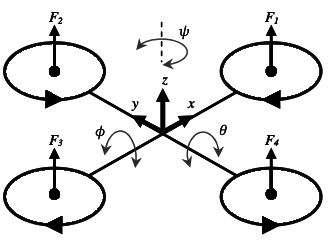
\includegraphics[width=0.6\textwidth]{./04-figuras/drone_diagram/drone_gray_separate1_white}
%    \fonte{Adaptado de \citeonline[p.~1]{Ariffanan2014}}
%    \label{fig:drone_diagram}
%\end{figure}

\begin{figure}[!htb]
    \centering
    \caption{Representação de um quadricóptero}
%    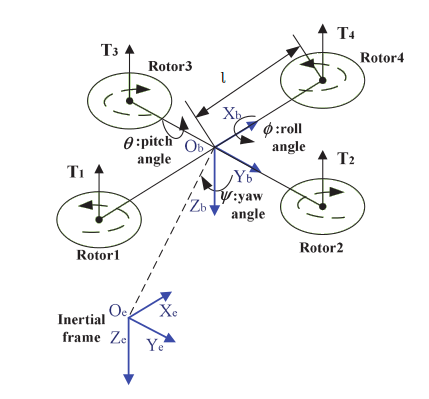
\includegraphics[width=0.6\textwidth]{./04-figuras/drone_diagram/drone_ref19_black_white}
    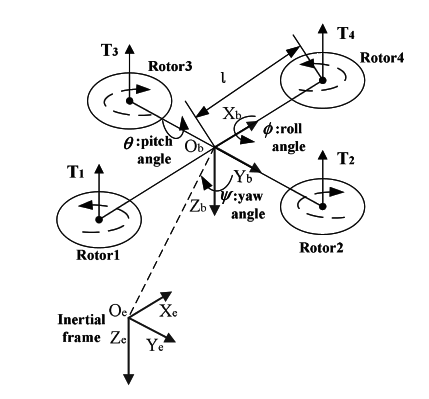
\includegraphics[width=0.7\textwidth]{./04-figuras/drone_diagram/drone_test_sep-1}
    \fonte{Adaptado de \citeonline{Gao2014Stability}}
    \label{fig:drone_diagram}
\end{figure}

Neste diagrama, $x$, $y$ e $z$ indicam a orientação dos eixos, $F_1$, $F_2$, $F_3$ e $F_4$ são as forças geradas pela propulsão de cada um dos motores. As variáveis $\phi$, $\theta$, e $\psi$ são os ângulos de rotação do quadricóptero em relação aos eixos $x$, $y$ e $z$ respectivamente. Estes ângulos são também chamados ângulos de \textit{roll} (rolamento), \textit{pitch} (arfagem) e \textit{yaw} (guinada), respectivamente. Além disto, o diagrama mostra ainda o sentido de rotação de cada um dos quatro rotores. Como se pode ver, os rotores dispostos sobre um mesmo eixo possuem um mesmo sentido de rotação. Desta forma, os rotores 1 e 3 (dispostos sobre o eixo $x$), giram no sentido horário. Já os rotores 2 e 4 (dispostos sobre o eixo $y$) giram no sentido anti-horário. Esta disposição dos rotores permite que os empuxos horizontais se anulem, possibilitando a estabilidade do quadricóptero quando submetido a uma ação de controle devida \cite[p.~1]{Ariffanan2014}.

A estabilidade de um quadricóptero, entretanto, assume mais de uma forma, sendo dividida em dois aspectos principais: altitude e atitude. O primeiro diz respeito ao posicionamento do quadricóptero sobre o eixo $z$ e seu controle é necessário tanto para possibilitar que ele se mantenha num estado estacionário quanto para fazer movimentações no plano XY numa altitude fixa, o que pode ser crucial se ele estiver sendo operado num ambiente limitado inferior e/ou superiormente por alguma espécie de barreira. Já o segundo aspecto, a atitude, se refere à estabilidade angular do quadricóptero, permitindo que sua orientação, representada pelos ângulos $\phi$, $\theta$, e $\psi$ seja controlada.

Uma vez descrito o comportamento geral do sistema, pode-se partir para a sua modelagem matemática. A modelagem retratada é a que foi desenvolvida por \citeonline{Balas2007} e é representada na Figura \ref{fig:diagrama-quadrotor-balas}

\begin{figure}[!htb]
    \centering
    \caption{Diagrama do sistema representando um quadrotor modelado por \citeonline{Balas2007}}
    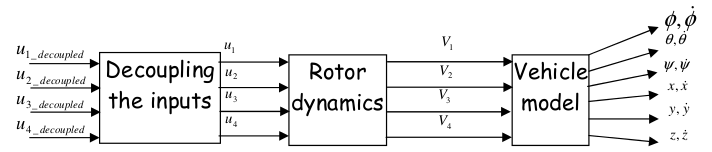
\includegraphics[width=1\textwidth]{./04-figuras/sistemas-nao-lineares/diagrama-quadrotor}
    \fonte{\citeonline[p.~49]{Balas2007}}
    \label{fig:diagrama-quadrotor-balas}
\end{figure}

\section{Modelagem Matemática}
\label{sec:dinamica-rotores}

O quadricóptero é controlado a partir da variação da velocidade dos seus quatro rotores, que são completamente independentes entre si. Desta forma, sendo $l$ o comprimento de cada haste a partir do centro geométrico do quadricóptero e considerando $v_i$ e $\tau_i$ respectivamente como o torque e o impulso do \textit{i}-ésimo rotor, podem-se considerar as entradas do sistema como sendo \cite[p.~4]{Balas2007}:
\begin{align}
u_1 &= \tau_1+\tau_2+\tau_3+\tau_4 \\
u_2 &= l(\tau_3-\tau_4) \\
u_3 &= l(\tau_1-\tau_2) \\
u_4 &= v_1+v_2+v_3+v_4
\end{align}
em que $u_1$ é o impulso total, $u_2$ é o momento de rolamento, $u_3$ é o momento de arfagem e $u_4$ é o momento de guinada.

Além disso, a aceleração em cada eixo pode ser representada por \cite[p.~5]{Balas2007}:
\begin{align}
\ddot{x} &= -\frac{sen(\theta)cos(\phi)}{m}u_1  \\
\ddot{y} &= \frac{sen(\phi)}{m}u_1  \\
\ddot{z} &= - \frac{cos(\theta)cos(\phi)}{m}u_1 +g
\end{align}
em que $\phi$ e $\theta$ são os ângulos em torno dos eixos $x$ e $y$ respectivamente, $m$ é a massa do quadricóptero e $g$ é a gravidade à qual ele é submetido.

Além das acelerações em cada eixo, é também necessário se definir a aceleração \textit{em torno} de cada eixo, ou seja, as acelerações angulares em torno de $x$, $y$ e $z$. Para tanto, assumindo que a estrutura do quadricóptero seja rígida, sendo $I_{xx}$, $I_{yy}$ e $I_{zz}$ o momento de inércia do quadricóptero ao longo dos eixos $x$, $y$ e $z$ respectivamente e considerando que os momentos de inércia ao longo de $x$ e $y$ se equivalem, as acelerações angulares podem ser representadas a partir das seguintes equações \cite[p.~6]{Balas2007}:
\begin{align}
\ddot{\phi} = -\dot{\psi}\dot{\theta}cos(\phi) + 
\frac{cos(\psi)}{I_{xx}}u_2 - 
\frac{sen(\psi)}{I_{yy}}u_3 + 
\frac{I_{yy}-I_{zz}}{I_{xx}}(\dot{\psi}-\dot{\theta}sen(\phi))\dot{\theta}cos(\phi)
\end{align}

\begin{align}
\begin{split}
\ddot{\theta} = \frac{\dot{\psi}\dot{\phi}}{cos(\phi)} +
\dot{\phi}\dot{\theta}tan(\phi) + 
\frac{sen(\psi)}{cos(\phi)I_{xx}}u_2 &+ 
\frac{cos(\psi)}{cos(\phi)I_{yy}}u_3 \\ 
&-\frac{I_{yy}-I_{zz}}{I_{xx}}(\psi-\dot{\theta}sen(\phi))\frac{\dot{\phi}}{cos(\phi)}
\end{split}
\end{align}

\begin{align}
\begin{split}
\ddot{\psi} = \dot{\phi}\dot{\psi}tan(\phi) +
\frac{\dot{\phi}\dot{\theta}}{cos(\phi)} + 
\frac{sen(\psi)tan(\phi)}{I_{xx}}u_2 &+ 
\frac{cos(\phi)tan(\psi)}{I_{yy}}u_3 + 
\frac{1}{I_{zz}}u_4 \\
&-\frac{I_{yy}I_{zz}}{I_{xx}} 
(\dot{\psi}-\dot{\theta}sen(\phi))\dot{\phi}tan(\phi)
\end{split}
\end{align}

Por fim, deve-se relacionar a velocidade de cada rotor \textit{i} ao impulso e torque sobre ele. Esta relação é dada por \cite[p.~7]{Balas2007}:
\begin{equation}
v_i = \tau_i(V_c+v_i)+0.125\rho bcR_p^4\omega_{m\textunderscore i}^2C_d
\end{equation}
sendo $v_i$ o torque sobre o rotor, $\tau_i$ o impulso atuando sobre ele, $V_c$ a velocidade vertical\footnote{A velocidade vertical do quadricóptero também é indicada por $\dot{z}$}, $v_i$ a velocidade induzida no motor, $\rho$ a densidade do ar, $b$ o número de pás, $c$ o comprimento delas, $R_p$ o raio da hélice, $C_d$ o coeficiente de arrasto e $\omega_{m\textunderscore i}$ a velocidade angular do rotor.

Após a modelagem de um sistema complexo como este, é de se desejar que se possa isolar a resposta de determinadas variáveis às entradas. Para tanto, pode-se utilizar o processo de desacoplamento de entradas.


\section{Desacoplamento das Entradas}
\label{sec:desacoplamento}

Para obter uma resposta isolada das variáveis do sistema a partir dos sinais de entrada dele, um bloco de desacoplamento foi modelado em \cite[p.~62]{Balas2007}. Neste caso, foram considerados os acoplamentos entre $\phi$, $\theta$, $\psi$ e $u_2$, $u_3$, $u_4$, relacionados da seguinte maneira:
\begin{align}
u_{2_{\textunderscore decoupled}} &= cos(\psi_{0})u_2 - \frac{I_{xx}sen(\psi_{0})}{I_{yy}}u_3 = I_{xx}\ddot{\phi} \\
u_{3_{\textunderscore decoupled}} &= \frac{sen(\psi_{0})I_{yy}}{cos(\phi_{0})I_{xx}}u_2 + \frac{cos(\psi_{0})}{cos(\phi_{0})}u_3 = I_{yy}\ddot{\theta} \\
u_{4_{\textunderscore decoupled}} &= \frac{I_{zz}sen(\psi_0)tan(\phi_0)}{I_{xx}}u_2 + \frac{I_{zz}cos(\psi_0)tan(\phi_0)}{I_{zz}}u_3 + u_4 = I_{zz}\ddot{\psi} 
\end{align}
em que $\dot{\phi_0}$, $\dot{\theta_0}$ e $\dot{\psi_0}$ são os ângulos no iniciais de rolamento, arfagem e guinada respectivamente; $\dot{\phi}$, $\dot{\theta}$ e $\dot{\psi}$ são os ângulos atuais de rolamento, arfagem e guinada; e $I_{xx}$, $I_{yy}$ e $I_{zz}$ são o momento de inércia em torno dos eixos \textit{x}, \textit{y} e \textit{z} respectivamente.

Como se pode ver pelas equações, aplicando esse desacoplamento obtêm-se as variáveis $u_{2_{\textunderscore decoupled}}$, $u_{3_{\textunderscore decoupled}}$ e $u_{4_{\textunderscore decoupled}}$ relacionadas aos ângulos $\phi$, $\theta$ e $\psi$ respectivamente e considerando o momento de inércia sobre os respectivos eixos, isolando assim a resposta das diferentes variáveis do sistema.

Além disso, a partir destas equações, podem-se representar essas transformações utilizando o formato matricial da seguinte maneira \cite[p.~62]{Balas2007}:
%Nesta estrutura, $u_1$ representa o empuxo total sobre o quadricóptero, $u_2$ representa o momento de \textit{roll} (em torno do eixo $x$), $u_3$ representa o momento de \textit{pitch} (em torno do eixo $y$) e $u_4$ representa o momento de \textit{yaw} (em torno do eixo $z$). $u_{2\textunderscore decoupled}$, $u_{3\textunderscore decoupled}$ e $u_{4\textunderscore decoupled}$ são combinações de $u_2$, $u_3$ e $u_4$ de tal forma que as entradas $u_{2\textunderscore decoupled}$, $u_{3\textunderscore decoupled}$ e $u_{4\textunderscore decoupled}$ tenham as mesmas direções que os ângulos de Euler, $\phi$, $\theta$ e $\psi$, respectivamente. A relação entre estas entradas é dada, em \cite[p.~49]{Balas2007} por:
\[
	\begin{bmatrix}
		u_{2} \\
		u_{3} \\
		u_{4}
	\end{bmatrix} = 
	\begin{bmatrix}
		cos(\psi_0) & sen(\psi_0)cos_(\phi_0)\frac{I_{xx}}{I_{yy}} & 
		0 \\
		
		-sen(\psi_{0})\frac{I_{yy}}{I_{xx}} &
		cos(\psi_{0})cos(\phi_{0}) &
		0 \\
		
		0 &
		-sen(\phi_{0})\frac{I_{zz}}{I_{yy}} &
		1
	\end{bmatrix}
	\begin{bmatrix}
		u_{2\textunderscore decoupled} \\
		u_{3\textunderscore decoupled} \\
		u_{4\textunderscore decoupled}
	\end{bmatrix}
\]

Após os processos de modelagem matemática do sistema e o devido desacoplamento de suas entradas, pode-se representar seu comportamento geral a partir dos espaços de estados, prática comum para descrever sistemas dinâmicos.
%$I_{xx}$, $I_{yy}$ e $I_{zz}$ representam o momento de inércia do quadricóptero ao longo dos eixos $x$, $y$ e $z$, respectivamente.

%\subsection{Funções de Transferência}
%\label{subsec:quadrotor-tfs}
%
%A partir da modelagem feita e já aplicando o desacoplamento implementado, o comportamento geral do quadrotor pode ser representado a partir de três funções de transferência distintas: uma sendo referente ao empuxo vertical; uma segunda, aos momentos de \textit{roll} e \textit{pitch}; e uma terceira, ao momento de \textit{yaw}.

Para se chegar a essas funções de transferência, o primeiro aspecto a ser considerado é que a relação entre a tensão e o torque é dado por uma aproximação feita a partir de \cite[p.~25]{Balas2007}:
\begin{equation}
H(s)=\frac{K}{1+\tau s}
\end{equation}
em que $\tau$ é uma constante de tempo $\tau = 0,314$ e que $K$ é o ganho CC do rotor definido como $K=0.045$N.m/V para exemplificar o sistema.

Desta forma, tem-se:
\begin{equation}
\frac{u_4}{V_1-V_2+V_3-V_4} = \frac{0,045}{0,314s + 1}
\end{equation}

%Assumindo um quadricóptero com massa $m$ igual a 2,354 g e uma aceleração $g$ igual a 9,81 N.
A partir dessas relações, a função de transferência obtida por \citeonline[p.~35]{Balas2007} para representar o empuxo vertical gerado pelos quatro rotores do quadrotor foi:
\begin{equation}
H(s) = \frac{u_1}{V_1+V_2+V_3-V_4} = \frac{2,105s-0,0425}{0,4895s^2+1,873s+1} N/V
\end{equation}

Já a função de transferência obtida para representar os momentos de \textit{roll} e de \textit{pitch} foi \cite[p.~35]{Balas2007}:
\begin{equation}
H(s) = \frac{u_2}{V_4-V_2} = \frac{u_3}{V_1-V_3} = l\frac{1,155s}{0,8696s^2+0,401s+1} Nm/V
\end{equation}

Por fim, a função de transferência obtida para representar o momento de \textit{yaw} foi \cite[p.~35]{Balas2007}:
\begin{equation}
H(s) =  \frac{u_4}{V_1-V_2+V_3-V_4} = \frac{0,045}{0,314s+1} Nm/V
\end{equation}

Uma forma alternativa à representação por funções de transferência é a representação no espaço de estados, que é mostrada na seção a seguir.


\subsection{Representação no Espaço de Estados}
\label{subsec:quadrotor-ss}

Como mostrado em \cite[p.~63]{Balas2007}, o sistema modelado, já incluindo o desacoplamento de entradas, pode ser representado da seguinte forma no espaço de estados.
\begin{align} \label{eq:space_state_equation_quadcopter}
	\dot{x} &= Ax + Bu \nonumber \\
	y		&= Cx + Du
\end{align}

Com o vetor de estados $X$ sendo dado por:
\begin{equation*}
X=
\left[ \begin{array}{@{}*{12}{c}@{}}
     x & y & z & \dot{x} & \dot{y} & \dot{z} & \phi & \theta & \psi & \dot{\phi} & \dot{\theta} & \dot{\psi}\\
\end{array} \right]^T
\end{equation*}

O vetor de entrada $U$ sendo:
\[ 
	U =
	\begin{bmatrix}
		u_1 & 
		u_{2\textunderscore decoupled} &
		u_{3\textunderscore decoupled} &
		u_{4\textunderscore decoupled}
	\end{bmatrix}^T
\]

E as matrizes A, B, C e D sendo definidas como:
\begin{equation*}
A =
\left[ \begin{array}{@{}*{12}{c}@{}}
     0 & 0 & 0 & 1 & 0 & 0 & 0 & 0  & 0 & 0 & 0 & 0 \\
     0 & 0 & 0 & 0 & 1 & 0 & 0 & 0  & 0 & 0 & 0 & 0 \\
     0 & 0 & 0 & 0 & 0 & 1 & 0 & 0  & 0 & 0 & 0 & 0 \\
     0 & 0 & 0 & 0 & 0 & 0 & 0 & -g & 0 & 0 & 0 & 0 \\
     0 & 0 & 0 & 0 & 0 & 0 & g & 0  & 0 & 0 & 0 & 0 \\
     0 & 0 & 0 & 0 & 0 & 0 & 0 & 0  & 0 & 0 & 0 & 0 \\
     0 & 0 & 0 & 0 & 0 & 0 & 0 & 0  & 0 & 1 & 0 & 0 \\
     0 & 0 & 0 & 0 & 0 & 0 & 0 & 0  & 0 & 0 & 1 & 0 \\
     0 & 0 & 0 & 0 & 0 & 0 & 0 & 0  & 0 & 0 & 0 & 1 \\
     0 & 0 & 0 & 0 & 0 & 0 & 0 & 0  & 0 & 0 & 0 & 0 \\
     0 & 0 & 0 & 0 & 0 & 0 & 0 & 0  & 0 & 0 & 0 & 0 \\
     0 & 0 & 0 & 0 & 0 & 0 & 0 & 0  & 0 & 0 & 0 & 0 \\
\end{array}\right]
\end{equation*}

\begin{equation*}
B =
\left[\begin{array}{@{}*{4}{c}@{}}
	0 & 0 & 0 & 0 \\
	0 & 0 & 0 & 0 \\
	0 & 0 & 0 & 0 \\
	0 & 0 & 0 & 0 \\
	0 & 0 & 0 & 0 \\
	-1/m & 0 & 0 & 0 \\
	0 & 0 & 0 & 0 \\
	0 & 0 & 0 & 0 \\
	0 & 0 & 0 & 0 \\
	0 & cos(\psi_0)/I_{xx} & -sen(\psi_0)/I_{yy} & 0 \\
	0 & sen(\psi_0)/(cos(\phi_0)I_{xx}) & cos(\psi_0)/(cos(\phi_0)I_{yy}) & 0\\
	0 & sin(\psi_0)tan(\phi_0)/I_{xx} & cos(\psi_0)
	tan(\phi_0)/I_{yy} & 1/I_{zz} \\
\end{array}\right]
\end{equation*}

\begin{equation*}
C =
\left[ \begin{array}{@{}*{12}{c}@{}}
	1 & 0 & 0 & 0 & 0 & 0 & 0 & 0 & 0 & 0 & 0 & 0 \\
	0 & 1 & 0 & 0 & 0 & 0 & 0 & 0 & 0 & 0 & 0 & 0 \\
	0 & 0 & 1 & 0 & 0 & 0 & 0 & 0 & 0 & 0 & 0 & 0 \\
	0 & 0 & 0 & 1 & 0 & 0 & 0 & 0 & 0 & 0 & 0 & 0 \\
	0 & 0 & 0 & 0 & 1 & 0 & 0 & 0 & 0 & 0 & 0 & 0 \\
	0 & 0 & 0 & 0 & 0 & 1 & 0 & 0 & 0 & 0 & 0 & 0 \\
	0 & 0 & 0 & 0 & 0 & 0 & 1 & 0 & 0 & 0 & 0 & 0 \\
	0 & 0 & 0 & 0 & 0 & 0 & 0 & 1 & 0 & 0 & 0 & 0 \\
	0 & 0 & 0 & 0 & 0 & 0 & 0 & 0 & 1 & 0 & 0 & 0 \\
	0 & 0 & 0 & 0 & 0 & 0 & 0 & 0 & 0 & 1 & 0 & 0 \\
	0 & 0 & 0 & 0 & 0 & 0 & 0 & 0 & 0 & 0 & 1 & 0 \\
	0 & 0 & 0 & 0 & 0 & 0 & 0 & 0 & 0 & 0 & 0 & 1 \\
\end{array}\right]
\end{equation*}

\begin{equation*}
D =
\left[\begin{array}{@{}*{4}{c}@{}}
	0 & 0 & 0 & 0 \\
	0 & 0 & 0 & 0 \\
	0 & 0 & 0 & 0 \\
	0 & 0 & 0 & 0 \\
	0 & 0 & 0 & 0 \\
	0 & 0 & 0 & 0 \\
	0 & 0 & 0 & 0 \\
	0 & 0 & 0 & 0 \\
	0 & 0 & 0 & 0 \\
	0 & 0 & 0 & 0 \\
	0 & 0 & 0 & 0 \\
	0 & 0 & 0 & 0 \\
\end{array}\right]
\end{equation*}
em que $g$ é a gravidade, $m$, a massa do quadricóptero e os ângulos $\phi_0$, $\theta_0$ e $\psi_0$ representam os ângulos iniciais em torno dos eixos $x$, $y$ e $z$ respectivamente. Além disto, $I_{xx}$, $I_{yy}$ e $I_{zz}$ representam o momento de inércia do quadricóptero ao longo destes mesmos eixos.

Como se pode perceber, a matriz C é uma matriz diagonal, o que implica no fato de a saída do sistema ser representada pelo vetor de estados.

Ao longo deste trabalho, essa foi a modelagem adotada para simular o sistema de um quadricóptero.
 % Sistemas nao lineares
%    %
% Documento: Trabalhos Relacionados
%

\chapter{Trabalhos Relacionados}

Na literatura, diversos são os exemplos de sistemas não lineares para os quais se desenvolvem diferentes tipos de controladores. Dentre estes tipos, encontramos os PD (Proporcional-Derivativo), PID (Proporcional-Integral-Derivativo), LQ (Linear-Quadrático), Fuzzy e ANFIS dentre outros sendo que este último tem se mostrado bastante presente para tentar atuar sobre diferentes tipos de sistemas.
%Controle Adaptativo L1

A grande quantidade de materiais propondo a implementação de controladores neuro-fuzzy se deve, em parte, ao fato de geralmente, para efetuar tal controle, não ser necessário se fazer uma modelagem matemática aprofundada do sistema que, em diversos casos, é de grande complexidade e, por isso, demandaria um grande esforço, sendo que em muitos casos os resultados não seriam tão bons quanto os desejados, além de oferecer ainda uma boa robustez ao controle.

Além do próprio controle de estabilidade de quadricópteros, podem-se encontrar exemplos de diversos sistemas que implementam controladores neuro-fuzzy. É o caso da implementação de um controlador para \textit{see and avoid\footnote{Ver e evitar (tradução nossa)}} (referente ao desvio de ocasionais obstáculos) de um \textit{drone}, como se pode encontrar em \citeonline{Olivares-Mendez2012}.
%
Já \citeonline{Guo2003}, propõem a implementação de um controlador neuro-fuzzy para controlar a estabilidade sobre o balanço de um barco. Os autores mostraram, ainda, que o controlador neuro-fuzzy obteve melhor resultado do que um controlador PID, chegando à conclusão de que controladores neuro-fuzzy são promissores para efetuar tal controle.

A grande gama de opções de controle sobre quadricópteros pode ser dividida em dois grupos principais: o controle \textit{tradicional} e o controle \textit{inteligente}. O primeiro diz respeito ao uso de técnicas consolidadas para controle baseado na atuação sobre eles a partir do conhecimento de sua modelagem, ao passo que o segundo se refere às técnicas de controle que envolvem componentes de Inteligência Computacional, agregando, por exemplo, representação de estados através de variáveis linguísticas e capacidade de aprendizagem.

%\section{Controle de Estabilidade de um Pêndulo Invertido}
%\label{sec:trab-rel-pendulo-invetido}
%
%Um dos sistemas dinâmicos não lineares intrinsecamente instáveis mais estudados é o de pêndulo invertido, sendo comumente usado em \textit{benchmarks} para verificar a eficácia de métodos de controle. 

%Outro caso em que se é muito comum a implementação deste tipo de controlador é para o controle de estabilidade de um pêndulo invertido. Diversas são as abordagens que se encontram na literatura.
%Um pêndulo invertido é um sistema instável não linear comumente usado em \textit{benchmarks} para verificar a eficácia de métodos de controle. 
%A figura \autoref{fig:inverted-pendulum-diagram} ilustra o modelo de um pêndulo invertido. Este sistema é composto de uma barra rígida colocada verticalmente sobre um carro. O objetivo do sistema é manter a barra em equilíbrio oscilatório, fazendo com que ela não caia \cite{Arai2014}.
\iffalse
\begin{figure}[!htb]
    \centering
    \caption{Modelo de um pêndulo invertido}
    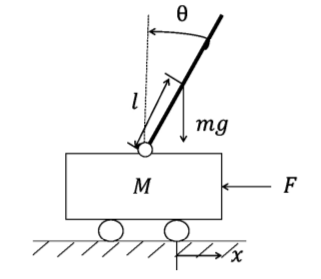
\includegraphics[width=0.4\textwidth]{./04-figuras/inverted-pendulum_diagram}
    \fonte{\cite[p.~416]{Arai2014}}
    \label{fig:inverted-pendulum-diagram}
\end{figure}

Na \autoref{fig:inverted-pendulum-diagram}, $M$ [$kg$] é a massa do carro, $m$ [$kg$] é a massa do pêndulo, $l$ [$m$] é metade do comprimento do pêndulo, $g$ [$m/s^2$] é a aceleração da gravidade e $\theta$ [$rad$] é o ângulo de desvio da barra em relação à posição vertical. O valor de cada variável de estado é calculada usando o método de Euller para um pequeno período de tempo $\tau$ [$s$].
\fi
\citeonline{Kim2000} compararam um controlador puramente LQR a um controlador híbrido, aliando o LQR a um controle neuro-fuzzy. A \autoref{fig:lqr-neuro-fuzzy-kim2000} mostra o esquema resultante. Neste modelo, a rede neural é configurada em paralelo ao controlador LQR. Este esquema consiste de um controlador LQR de ganho fixo que faz o sistema como um todo estável e um controlador realimentado que atualiza seus pesos internos para gerar o sinal de controle $u_{FN}$ contribuindo para a redução de tempo de convergência do sistema.

\begin{figure}[!htb]
    \centering
    \caption{Diagrama do controlador híbrido LQR-Neuro-Fuzzy implementado em \cite{Kim2000}}
    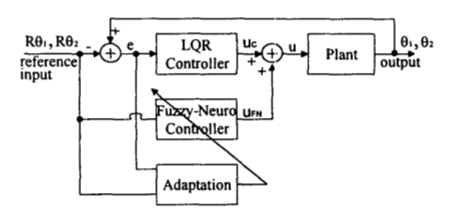
\includegraphics[width=0.6\textwidth]{./04-figuras/lqr_neuro_fuzzy_pendulum}
    \fonte{\cite[p.~416]{Kim2000}}
    \label{fig:lqr-neuro-fuzzy-kim2000}
\end{figure}

Resultados de simulação mostraram que o controlador híbrido LQR-Neuro-Fuzzy obteve menor erro na fase inicial de treinamento se comparado ao controlador LQR. Além disto, os resultados mostraram que o controlador proposto é mais eficiente que o LQR, obtendo melhor tempo de convergência.

\citeonline{Omatu1994} também propuseram um controlador híbrido aliando os controles LQR e Fuzzy. Neste caso, entretanto, os controladores operam em momentos diferentes. O controlador neuro-fuzzy atua sobre o sistema até que o pêndulo se aproxime da posição vertical. A partir de um ponto de referência, o controle passa a ser efetuado pelo controlador LQR. Neste caso, mais uma vez a inserção de um controle por neuro-fuzzy contribiu para a boa resposta do sistema.

Em \cite{Alata2001}, outro tipo de controlador híbrido LQR-Neuro-Fuzzy é proposto. Neste caso, os ganhos em diferentes regiões de operação são calculados usando o método LQR. Esses ganhos são tabulados com os estados correspondentes do ponto de operação. Então, um agrupamento subtrativo e o ANFIS são usados para contruir a base de dados e a base de regras do sistema de inferências fuzzy. Isto fornece um mecanismo suave de transição de um ponto de operação para outro. A eficácia da abordagem proposta foi provada por resultados experimentais de um pêndulo invertido.

Já \citeonline{Arai2014} utilizaram uma abordagem diferente, implementando um controlador puramente CVNF (\textit{Complex-Valued Neuro-Fuzzy}\footnote{Neuro-Fuzzy com Valores Complexos, tradução nossa}), que diz repeito a uma expansão de um controlador neuro-fuzzy para o conjunto dos números complexos. Algumas das vantagens deste método são que ele apresenta menor tempo de treinamento e, ainda assim, uma melhor precisão de treinamento. Utilizando-o, os autores obtiveram um resultado melhor do que usando um controlador Neuro-Fuzzy, possuindo melhor tempo de resposta e, ainda, um maior alcance de ângulos iniciais que podem ser compensados.


%\subsection{Métodos de Controle Tradicional de Helicópteros Quadrotores}
%\label{sec:trab-rel-quadrotores-sub-trad}
\section{Controle Tradicional de Quadricópteros}
\label{sec:trab-rel-tradicional}

Esta seção aborda diferentes propostas de controladores tradicionais para quadricópteros visando a contextualização do estado da arte para depois se poder comparar alguns resultados das técnicas tradicionais e inteligentes de controle para esse sistema.

Em \cite{Razinkova2014}, foi proposto um controlador PD para a descrição adequada das trajetórias definidas de um quadricóptero \textit{Indoor}. Para permitir um funcionamento adequado \textit{Outdoor}, foi integrado ao controlador PD um controle adaptativo, adicionando termos ao controlador convencional, de forma a permitir o ajuste correto da trajetória do quadricóptero quando submetido a distúrbios nos eixos X e Y (plano horizontal). Os resultados mostraram que o controlador adaptativo melhorou consideravelmente o controle de trajetória do \textit{drone}, reduzindo em 64\% o erro de posicionamento para os casos de trajetória em linha reta ao longo do plano XY, e em 72\% para os casos de trajetória circular sobre o plano XY. Segundo os autores, este resultado representa uma melhora significativa, uma vez que o controlador resultante possui uma arquitetura simples e não requer computação extensiva, o que é indesejado para qualquer controle de sistema, especialmente para UAVs, devido à sua limitação de bateria.

Em \cite{Mustapa2014} é proposto um controlador PID para efetuar o controle visando a estabilidade da altitude de um quadricóptero. Neste trabalho, foi utilizado um modelo matemático desenvolvido previamente para descrever o comportamento do sistema. Para ajustar os parâmetros do controlador PID, foi necessário realizar um experimento para determinar o momento de inércia do drone. Uma vez levantados os valores necessários, um controlador PID foi ajustado e se mostrou eficiente. A simulação do sistema foi realizada no Matlab Simulink\textsuperscript{\textregistered}.

\citeonline{Khatoon2014} também propuseram um controlador PID para controlar a estabilidade em altitude de um drone, mantendo a posição no eixo XY constante, mesmo esta altitude sendo uma variável muito sensível a mudanças em outros parâmetros. No trabalho, é mostrado que um controlador PID sozinho é capaz de exercer tal controle com robustez. A escolha deste controlador se deu graças à sua robustez e facilidade de modelagem. Entretanto, é também apontado pelos autores que, apesar da simplicidade para se modelar um controlador PID, isto requer uma modelagem do sistema como um todo, o que não é fácil, devido à sua estrutura complexa, suas dinâmicas não lineares e sua natureza subatuada. O sistema modelado para o drone mostrou ser altamente instável, justificando a necessidade de um controlador. A partir de extensivas simulações no MATLAB/Simulink, o sistema desenvolvido se mostrou bem sucedido, implementando de fato um controle robusto de altitude para um helicóptero quadricóptero.

Além desses controladores que aplicam técnicas tradicionais, são também vários os exemplos de trabalhos que exploram o controle inteligente de quadricópteros.

%\subsection{Métodos de Controle Inteligente de Helicópteros Quadrotores}
%\label{sec:trab-rel-quadrotores-sub-ia}
\section{Controle Inteligente de Quadricópteros}
\label{sec:trab-rel-inteligente}

Além das técnicas de controle tradicionais, encontram-se também na literatura diversas abordagens para a construção de controladores de estabilidade para \textit{drones} utilizando técnicas da Inteligência Computacional. As propostas vão do uso de algoritmos de otimização (e.g.\ algoritmos genéticos, PSO) ao uso de sistemas neuro-\textit{fuzzy} expandido para o espaço dos números complexos.

%22
%\cite{Rezazadeh2013}
Em \cite{Rezazadeh2013}, é proposto um controlador neuro-\textit{fuzzy} (ANFIS) para o controle estabilizante de altitude de um quadricóptero. O módulo \textit{fuzzy} acoplado a um controlador PID é usado para controlar a atitude. Os controladores \textit{fuzzy} atualizam os ganhos do PID \textit{online} para produzir uma resposta apropriada. A saída é calculada diretamente pelo ajuste dos pesos das entradas de acordo com as regras de inferência \textit{fuzzy}. Estas regras, que são a base de conhecimento, são determinadas por um algoritmo computacional baseado em redes neurais. O controlador proposto foi comparado a um simples controlador PID e, a partir de simulações, foi mostrado que se obteve melhor resposta, por exemplo, tendo em vista o tempo de assentamento e a sobrelevação. Outro resultado obtido foi de que o controlador ANFIS é capaz de estabilizar o sistema quando exposto a perturbações externas.

%34
%\cite{Mahfouz2013}
Em \cite{Mahfouz2013}, foi proposto um controlador parecido. Neste trabalho, também foi sugerido um controlador ANFIS que, juntamente com um algoritmo genético, ajusta os pesos de um controlador PID. Mais uma vez, foi obtido sucesso com o controlador desenvolvido, sendo possível garantir a estabilidade de um \textit{drone} mesmo quando sujeito a perturbações. No trabalho, foi mostrado que a sobrelevação do controlador ANFIS é menor do que a do PID. Além disto, o erro de regime permanente no caso do ANFIS é zero, enquanto, no caso do controaldor PID, não o é. Uma conclusão muito importante a que se chega é que, do ponto de vista de robustez, os dois controladores são efetivos; do ponto de vista de performance, o ANFIS é melhor que o PID.

%14
%\cite{Maj2013}
Em \cite{Maj2013} é proposto um controle de estabilidade para um quadricóptero usando lógica \textit{fuzzy}. Neste trabalho, três controladores \textit{fuzzy} são usados: um para cada um dos dois eixos horizontais (\textit{x} e \textit{y}) e mais um controlador geral para todo o sistema. Com isto, o erro angular e a aceleração são as variáveis linguísticas. Em ambos os casos, são usados cinco termos linguísticos: muito negativo (NL), pouco negativo (NS), zero (Z), pouco positivo (PS) e muito positivo (PL). Os conjuntos NS, Z e PS são triangulares enquanto os conjuntos NL e PL são trapezoidais, como mostra a Figura \ref{fig:Maj2013_fuzzy_sets}. 

\begin{figure}[!htb]
    \centering
    \caption{Conjuntos \textit{fuzzy} usados em \cite{Maj2013}; a) erro de posição; b) erro de giro }
    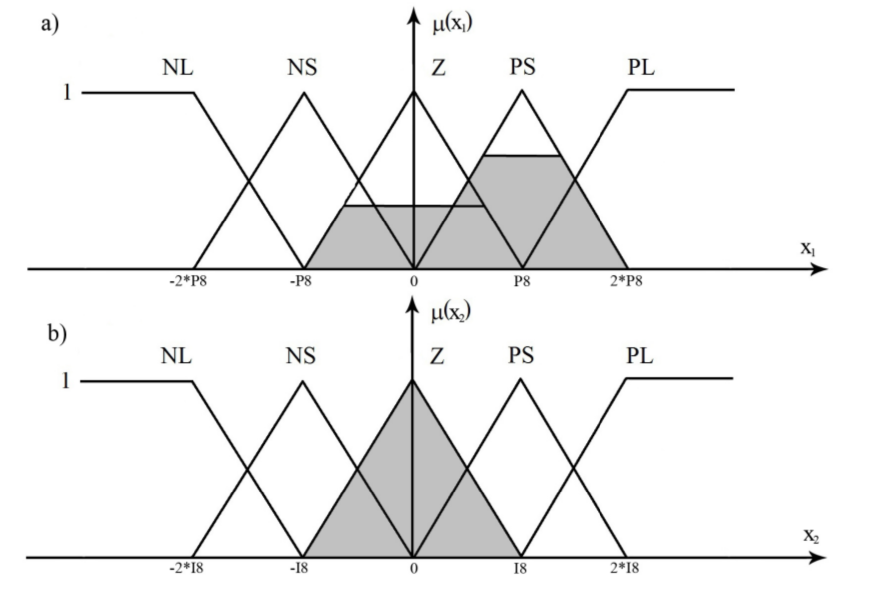
\includegraphics[width=0.6\textwidth]{./04-figuras/Maj2013_fuzzy_sets}
    \fonte{\cite{Maj2013}}
    \label{fig:Maj2013_fuzzy_sets}
\end{figure}

O bloco de fuzzificação calcula o grau de confiança dos conjuntos de entrada e um segundo bloco executa a inferência, que calcula o grau de confiança dos conjuntos de saída. As operações MIN e MAX são usadas como operadores AND e OR respectivamente para os conjuntos \textit{fuzzy}. O conjunto de regras utilizadas é mostrado no Quadro \ref{qua:Maj2013_table_rules_inference}.
% e os conjuntos \textit{fuzzy} antes da defuzzificação são mostrados na Figura \ref{fig:Maj2013_fuzzy_sets_output}.

\begin{quadro}[!htb]
    \centering
    \caption{Regras de inferência fuzzy usadas em \cite{Maj2013}\label{qua:Maj2013_table_rules_inference}}
    % \begin{tabular}{|p{3cm}|p{3cm}|p{3cm}|p{3cm}|p{3cm}|p{3cm}|}
    \begin{tabular}{c|c|c|c|c|c|}
        \cline{2-6}
        & \multicolumn{5}{c|}{\textbf{Erro de Giro}} \\
        
        \hline
        \multicolumn{1}{ |c| }{\textbf{Erro Angular}} & 
                            \textbf{NL} &
                            \textbf{NS} & 
                            \textbf{Z}  & 
                            \textbf{PS} & 
                            \textbf{PL}  \\
        \hline
        \multicolumn{1}{ |c| }{\textbf{NL}} & 
                            PL &
                            PL & 
                            PL & 
                            PS & 
                            Z  \\
        \hline
        \multicolumn{1}{ |c| }{\textbf{NS}} & 
                            PL &
                            PL & 
                            PS & 
                            Z  & 
                            NS \\

        \hline
        \multicolumn{1}{ |c| }{\textbf{Z}} & 
                            PL &
                            PS & 
                            Z  & 
                            NS & 
                            NL \\
        \hline
        \multicolumn{1}{ |c| }{\textbf{PS}} & 
                            PS &
                            Z  & 
                            NS & 
                            NL & 
                            NL \\
        \hline
        \multicolumn{1}{ |c| }{\textbf{PL}} & 
                            Z  &
                            NS & 
                            NL & 
                            NL & 
                            NL \\
        \hline
    \end{tabular}
    \fonte{Adaptado de \citeonline{Maj2013}}
\end{quadro}












% \begin{quadro}[!htb]
%     \centering
%     \caption{Tabela de regras para inferência.\label{qua:Maj2013_table_rules_inference}}
%     % \begin{tabular}{|p{3cm}|p{3cm}|p{3cm}|p{3cm}|p{3cm}|p{3cm}|}
%     \begin{tabular}{c|c|c|c|c|c|}
%         \cline{2-6}
%         & \multicolumn{5}{c|}{\textbf{Erro de Giro}} \\
%         % \cline{2-6}
        
%         \hline
%         \multicolumn{1}{ |c| }{\textbf{Erro Angular}} & 
%                             \textbf{NL} &
%                             \textbf{NS} & 
%                             \textbf{Z} & 
%                             \textbf{PS} & 
%                             \textbf{PL} \\
%         \hline
%             % \textbf{Erro Angular} & 
%             % \textbf{NL} &
%             % \textbf{NS} & 
%             % \textbf{Z} & 
%             % \textbf{PS} & 
%             % \textbf{PL} \\
%         % \hline
%         % a & b & c & d & e & f \\
%         % \hline
%     \end{tabular}
%     \fonte{Adaptado de \citeonline{Maj2013}}
% \end{quadro}

















%backup
% \begin{quadro}[!htb]
%     \centering
%     \caption{Tabela de regras para inferência.\label{qua:Maj2013_table_rules_inference}}
%     % \begin{tabular}{|p{3cm}|p{3cm}|p{3cm}|p{3cm}|p{3cm}|p{3cm}|}
%     \begin{tabular}{|c|c|c|c|c|c|}
%         \hline
%             \textbf{Erro Angular/Erro de Giro} & 
%             \textbf{NL} &
%             \textbf{NS} & 
%             \textbf{Z} & 
%             \textbf{PS} & 
%             \textbf{PL} \\
%         \hline
%         a & b & c & d & e & f \\
%         \hline
%     \end{tabular}
%     \fonte{Adaptado de \citeonline{Maj2013}}
% \end{quadro}



%\begin{figure}[!htb]
%    \centering
%    \caption{Conjuntos fuzzy antes da defuzzificação usados em \cite{Maj2013} }
%    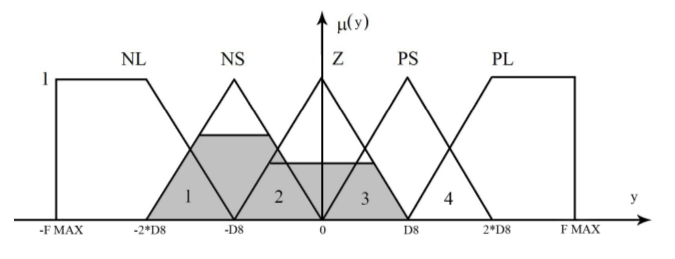
\includegraphics[width=0.6\textwidth]{./04-figuras/Maj2013_fuzzy_sets_output}
%    \fonte{\cite{Maj2013}}
%    \label{fig:Maj2013_fuzzy_sets_output}
%\end{figure}

Os autores obtiveram sucesso no controle estabilizante do \textit{drone}, mas somente utilizando um bloco integrador. Apesar de os reguladores e motores serem do mesmo tipo, algumas características deles são levemente diferentes. Como consequência, os motores não giram todos na mesma velocidade causando uma inclinação do quadricóptero. Esta inclinação pode ser corrigida com o uso de um bloco integrador. Desta forma, foi observado que um controlador puramente \textit{fuzzy} pode não ser suficiente para lidar com esta situação mas que, acoplando um bloco integrador, o sistema certamente pode ser estabilizado.
%A solução encontrada foi, portanto, implementar um controlador híbrido, que se mostrou eficiente para tal propósito.

%06
%\cite{Coza2006}
\citeonline{Coza2006} propuseram um controlador \textit{fuzzy} adaptativo para controlar a estabilidade de um quadricóptero \textit{Outdoor}. A escolha deste tipo de controlador se deu graças a inconvenientes apresentados por outros métodos. Controle adaptativo pode ser apropriado, mas requer conhecimento aprofundado do tipo de não linearidades nas dinâmicas do sistema. Um SMC (\textit{Sliding Mode Control}\footnote{Controle por Modos Deslizantes (tradução nossa).}) pode ser apropriado mas pode causar chaveamento indesejado no sinal de controle. Sistemas de controle com RNAs podem ser apropriados, mas requerem intenso esforço computacional para operar.

A abordagem utilizada em \cite{Coza2006} se baseia na ideia de que diferentes conjuntos de centros de decodificação são capazes de aproximar uniformemente a mesma função não linear. Desta forma, é usado treino supervisionado sobre os centros alternados: o erro do estado treina o centro de controle e a diferença na saída treina os centros alternados. A partir de simulações, mostrou-se que o resultado obtido foi um controle estável, computacionalmente eficiente e teoricamente robusto a perturbações. Entretanto, em uma das situações de simulações de perturbações por vento, o controlador teve de sacrificar a bom desempenho computacional para prevenir o desvio de centro. Ainda assim, foi mostrado que um modelo \textit{fuzzy} adaptativo usando atualização de controle e centro pode ser usado para cada eixo de rotação: X, Y e Z. Para tanto, apenas quatro funções de pertinência Gaussianas foram usadas para cada entrada de controle.

%10
%\cite{Rabhi2011}
Em \cite{Rabhi2011} uma outra abordagem é utilizada. Neste caso, os autores propuseram um controlador Fuzzy TSK (Takagi-Sugeno-Kang) para controlar a estabilidade de um quadricóptero. O controlador foi modelado usando ferramentas matemáticas, mais especificamente LMIs (\textit{Linear Matrix Inequalities}\footnote{Desigualdades Matriciais Lineares (tradução nossa).}) e modelado empregando PDC (\textit{Parallel Distributed Compensation}\footnote{Compensação Paralela Distribuída (tradução nossa).}). O objetivo foi projetar um controlador fuzzy realimentado para garantir a estabilidade do sistema com robustez. Simulações mostram que o controlador projetado garante, de fato, a estabilidade global do sistema em malha fechada.

%13
%\cite{Sheikhpour2013}
\citeonline{Sheikhpour2013} seguiram a mesma linha de \citeonline{Rabhi2011} e propuseram um controlador fuzzy TSK para estabilização de altura de um quadricóptero. Mais uma vez, a técnica PDC foi utilizada para projetar o controlador de realimentação. Neste trabalho, entretanto, o controle de estabilidade levou em conta especificações de desempenho como taxa de decaimento e restrições na entrada. Como ambas condições podem ser representadas por LMIs, elas também foram usadas neste caso, sendo mais complexas por lidar com as restrições dadas. Foi mostrado que simultaneamente à resolução das LMIs, foi projetado não apenas um controlador \textit{fuzzy} estável mas também com inclusão de velocidade de resposta desejada e restrições na entrada de altitude no controlador. Os resultados obtidos em simulações mostram a viabilidade desta abordagem.

%16
%\cite{JavidiNiroumand2013}
\citeonline{JavidiNiroumand2013} propuseram uma forma alternativa de controlador também usando a lógica fuzzy. Na abordagem utilizada, primeiramente foi derivado um modelo dinâmico não linear de um quadricóptero e então foi desenvolvido um controlador híbrido usando métodos de controle tradicionais e inteligentes para estabilização de dinâmicas rotacionais. A técnica IBS (\textit{Integral Backstepping}) é um poderoso método de controle tradicional amplamente utilizado para tal tipo de sistema mas encontrar o coeficiente apropriado do algoritmo é um trabalho crítico. Neste caso, esse problema foi resolvido usando um método de controle \textit{fuzzy}. Foi mostrado nos resultados que o método IBS possui domínio de atração mais amplo em comparação a métodos de controle lineares como o PID e uma melhor convergência. Foi mostrado ainda que ambos controladores IBS e \textit{Fuzzy} IBS foram capazes de controlar o sistema de forma apropriada. Entretanto, o controlador FIBS (\textit{Fuzzy Integral Backstepping}) obteve resultados levemente superiores ao IBS além de ter apresentado benefícios como uma melhor rejeição a perturbações e melhor robustez.
%\footnote{\textit{Backstepping} Integral, tradução nossa}
%\footnote{Backstepping Integral Fuzzy, tradução nossa}

%20
%\cite{Ariffanan2014}
Já em \cite{Ariffanan2014}, foi proposto um controlador FSBC (\textit{Fuzzy Supervisory Backstepping Controller}\footnote{Controlador por \textit{Backstepping Fuzzy} Supervisionado (tradução nossa).}). O controlador projetado consiste em controlador de \textit{backstepping} que pode selecionar automaticamente seus parâmetros \textit{on line} por um mecanismo de supervisão \textit{fuzzy}. O critério de estabilidade para a estabilização do quadricóptero é provada pelo teorema de Lyapunov. Extensivas simulações mostram a eficácia desta abordagem, apontando que uma alta precisão no transiente e no tempo de controle foram alcançados. Além disto, os resultados indicam que a técnica proposta pode estabilizar quadricópteros com melhor desempenho se comparado a técnicas de estabilização lineares.

%
%19
%\cite{Gao2014Stability}
Em \cite{Gao2014Stability}, é proposto um outro tipo de controlador híbrido. Neste caso, o controle é feito a partir de um sistema composto por dois controladores independentes: um controlador \textit{Backstepping} e um segundo controlador \textit{Fuzzy} PID Adaptativo, que alia a lógica \textit{fuzzy} a um controlador PID. Quando o quadricóptero voa em boas condições, o controle de estabilidade é assumido pelo controlador \textit{Backstepping}. Quando o quadricóptero encontra vento ou outro fator de perturbação durante o voo, o controlador \textit{Fuzzy} PID Adaptativo\footnote{O controlador \textit{Fuzzy} PID Adaptativo é um controlador PID que emprega o Sistema de Inferência \textit{Fuzzy} (FIS) para ajustar os parâmetros $K_p$, $K_i$, $K_d$, ganhos proporcional, integral e derivativo respectivamente.} é usado para estabilizá-lo. . O controlador proposto alcançou sucesso nos testes realizados, permitindo que se complete a trajetória sem que perturbações afetem a precisão do controle. Com isso, o Sistema de Inferência \textit{Fuzzy} se mostrou eficiente para ajustar os ganhos do controlador PID de forma a possibilitar o controle eficiente do quadricóptero.

%A \autoref{fig:Gao2014Stability_block_diagram} mostra o diagrama de blocos representando o controlador Fuzzy PID.
%
%\begin{figure}[!htb]
%    \centering
%    \caption{Diagrama de blocos do controlador híbrido usando em \cite{Gao2014Stability}}
%    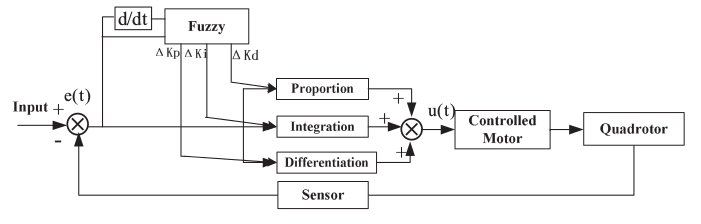
\includegraphics[width=0.9\textwidth]{./04-figuras/Gao2014Stability_block_diagram}
%    \fonte{\citeonline{Gao2014Stability}}
%    \label{fig:Gao2014Stability_block_diagram}
%\end{figure}
%
%Em relação à estrutura fuzzy, há duas entradas para a inferência fuzzy: o erro e a derivada do erro. São três saídas, cada uma sendo um parâmetro do controlador PID $\Delta kp$, $\Delta ki$ e $\Delta kd$. O universo de discurso foi normalizado e dividido em sete subconjuntos fuzzy. Os termos linguísticos foram definidos da seguinte forma: NB, negativo grande; NM, negativo médio; NS, negativo pequeno; ZO, aproximadamente zero; PS, positivo pequeno; PM, positivo médio; e PB, positivo grande. Os conjuntos fuzzy para cada variável de entrada consistem de sete variáveis linguísticas: $e$ = \{NB, NM, NS, ZO, PS, PM, PB\}, $e_c$ = \{NB, NM, NS, ZO, PS, PM, PB\}. As variáveis linguísticas das saídas são atribuídas da seguinte forma: $\Delta kp$ = \{ZO, PS, PM, PB\}, $\Delta ki$ = \{ZO, PS, PM, PB\}, $\Delta kp$ = \{ZO, PS, PM, PB\}. As regras de inferência Fuzzy para as variáveis de saída $\Delta kp$, $\Delta ki$ e $\Delta kd$ são mostradas nos Quadros \ref{qua:Gao2014Stability_table_rules_inference_kp}, \ref{qua:Gao2014Stability_table_rules_inference_ki} e \ref{qua:Gao2014Stability_table_rules_inference_kd} respectivamente.
%
%\begin{quadro}[!htb]
    \centering
    \caption{Regras de inferência fuzzy usadas em \cite{Gao2014Stability} para a variável $\Delta K_p$\label{qua:Gao2014Stability_table_rules_inference_kp}}
    \begin{tabular}{c|c|c|c|c|c|c|c|}
        \cline{2-8}
        & \multicolumn{7}{c|}{\textbf{$\Delta E_c$}} \\
        
        %cabeçalho
        \hline
        \multicolumn{1}{ |c| }{\textbf{E}} & 
                            \textbf{NB} &
                            \textbf{NN} & 
                            \textbf{NS} & 
                            \textbf{ZO} & 
                            \textbf{PS} & 
                            \textbf{PM} & 
                            \textbf{PB} \\
        \hline
        %NB OK
        \multicolumn{1}{ |c| }{\textbf{NB}} & 
                            PB &
                            PM &
                            ZO &
                            ZO &
                            ZO &
                            PM &
                            PB \\
        \hline
        %NM OK
        \multicolumn{1}{ |c| }{\textbf{NM}} & 
                            PB &
                            PM &
                            ZO &
                            ZO &
                            ZO &
                            PM &
                            PB \\
        \hline
        %NS OK
        \multicolumn{1}{ |c| }{\textbf{NS}} & 
                            PB &
                            PB &
                            PS &
                            ZO &
                            PS &
                            PB &
                            PB \\
        \hline
        %ZO OK
        \multicolumn{1}{ |c| }{\textbf{ZO}} & 
                            PB &
                            PB &
                            PS &
                            ZO &
                            PS &
                            PB &
                            PB \\
        \hline
        %PS OK
        \multicolumn{1}{ |c| }{\textbf{PS}} & 
                            PB &
                            PB &
                            PS &
                            ZO &
                            PS &
                            PB &
                            PB \\
        \hline
        %PM OK
        \multicolumn{1}{ |c| }{\textbf{PM}} & 
                            PB &
                            PM &
                            ZO &
                            ZO &
                            ZO &
                            PM &
                            PB \\
        \hline
        %PB OK
        \multicolumn{1}{ |c| }{\textbf{PB}} & 
                            PB &
                            PM &
                            ZO &
                            ZO &
                            ZO &
                            PM &
                            PB \\
        \hline

        % \multicolumn{1}{ |c| }{\textbf{NB}} & 
        %                     PB/ZO/PB &
        %                     PB/ZO/PB &
        %                     PB/ZO/PB &
        %                     PB/ZO/PB &
        %                     PB/ZO/PB &
        %                     PB/ZO/PB &
        %                     PB/ZO/PB \\
        % \hline

    \end{tabular}
    \fonte{Adaptado de \citeonline{Gao2014Stability}}
\end{quadro}






%
%\begin{quadro}[!htb]
    \centering
    \caption{Regras de inferência fuzzy usadas em \cite{Gao2014Stability} para a variável $\Delta K_i$\label{qua:Gao2014Stability_table_rules_inference_ki}}
    \begin{tabular}{c|c|c|c|c|c|c|c|}
        \cline{2-8}
        & \multicolumn{7}{c|}{\textbf{$\Delta E_c$}} \\
        
        %cabeçalho
        \hline
        \multicolumn{1}{ |c| }{\textbf{E}} & 
                            \textbf{NB} &
                            \textbf{NN} & 
                            \textbf{NS} & 
                            \textbf{ZO} & 
                            \textbf{PS} & 
                            \textbf{PM} & 
                            \textbf{PB} \\
        \hline
        %NB OK
        \multicolumn{1}{ |c| }{\textbf{NB}} & 
                            ZO &
                            ZO &
                            ZO &
                            PS &
                            ZO &
                            ZO &
                            ZO \\
        \hline
        %NM OK
        \multicolumn{1}{ |c| }{\textbf{NM}} & 
                            ZO &
                            ZO &
                            ZO &
                            PS &
                            ZO &
                            ZO &
                            ZO \\
        \hline
        %NS OK
        \multicolumn{1}{ |c| }{\textbf{NS}} & 
                            ZO &
                            ZO &
                            PS &
                            PS &
                            PS &
                            ZO &
                            ZO \\
        \hline
        %ZO OK
        \multicolumn{1}{ |c| }{\textbf{ZO}} & 
                            ZO &
                            ZO &
                            PS &
                            PS &
                            PS &
                            ZO &
                            ZO \\
        \hline
        %PS OK
        \multicolumn{1}{ |c| }{\textbf{PS}} & 
                            ZO &
                            ZO &
                            PS &
                            PS &
                            PS &
                            ZO &
                            ZO \\
        \hline
        %PM OK
        \multicolumn{1}{ |c| }{\textbf{PM}} & 
                            ZO &
                            ZO &
                            ZO &
                            PS &
                            ZO &
                            ZO &
                            ZO \\
        \hline
        %PB OK
        \multicolumn{1}{ |c| }{\textbf{PB}} & 
                            ZO &
                            ZO &
                            ZO &
                            PS &
                            ZO &
                            ZO &
                            ZO \\
        \hline

        % \multicolumn{1}{ |c| }{\textbf{NB}} & 
        %                     PB/ZO/PB &
        %                     PB/ZO/PB &
        %                     PB/ZO/PB &
        %                     PB/ZO/PB &
        %                     PB/ZO/PB &
        %                     PB/ZO/PB &
        %                     PB/ZO/PB \\
        % \hline

    \end{tabular}
    \fonte{Adaptado de \citeonline{Gao2014Stability}}
\end{quadro}






%
%\begin{quadro}[!htb]
    \centering
    \caption{Regras de inferência fuzzy usadas em \cite{Gao2014Stability} para a variável $\Delta K_d$\label{qua:Gao2014Stability_table_rules_inference_kd}}
    \begin{tabular}{c|c|c|c|c|c|c|c|}
        \cline{2-8}
        & \multicolumn{7}{c|}{\textbf{$\Delta E_c$}} \\
        
        %cabeçalho
        \hline
        \multicolumn{1}{ |c| }{\textbf{E}} & 
                            \textbf{NB} &
                            \textbf{NN} & 
                            \textbf{NS} & 
                            \textbf{ZO} & 
                            \textbf{PS} & 
                            \textbf{PM} & 
                            \textbf{PB} \\
        \hline
        %NB OK
        \multicolumn{1}{ |c| }{\textbf{NB}} & 
                            PB &
                            PB &
                            PM &
                            PS &
                            PM &
                            PB &
                            PB \\
        \hline
        %NM OK
        \multicolumn{1}{ |c| }{\textbf{NM}} & 
                            PB &
                            PB &
                            PM &
                            PS &
                            PM &
                            PB &
                            PB \\
        \hline
        %NS OK
        \multicolumn{1}{ |c| }{\textbf{NS}} & 
                            PB &
                            PM &
                            PS &
                            ZO &
                            PS &
                            PM &
                            PB \\
        \hline
        %ZO OK
        \multicolumn{1}{ |c| }{\textbf{ZO}} & 
                            PB &
                            PM &
                            PS &
                            ZO &
                            PS &
                            PM &
                            PB \\
        \hline
        %PS OK
        \multicolumn{1}{ |c| }{\textbf{PS}} & 
                            PB &
                            PM &
                            PS &
                            ZO &
                            PS &
                            PM &
                            PB \\
        \hline
        %PM OK
        \multicolumn{1}{ |c| }{\textbf{PM}} & 
                            PB &
                            PB &
                            PM &
                            ZO &
                            PM &
                            PB &
                            PB \\
        \hline
        %PB OK
        \multicolumn{1}{ |c| }{\textbf{PB}} & 
                            PB &
                            PB &
                            PM &
                            PS &
                            PM &
                            PB &
                            PB \\
        \hline

        % \multicolumn{1}{ |c| }{\textbf{NB}} & 
        %                     PB/ZO/PB &
        %                     PB/ZO/PB &
        %                     PB/ZO/PB &
        %                     PB/ZO/PB &
        %                     PB/ZO/PB &
        %                     PB/ZO/PB &
        %                     PB/ZO/PB \\
        % \hline

    \end{tabular}
    \fonte{Adaptado de \citeonline{Gao2014Stability}}
\end{quadro}







%O controlador proposto alcançou sucesso nos testes realizados, permitindo que se complete a trajetória sem que perturbações afetem a precisão de controle. O Sistema de Inferência \textit{Fuzzy} se mostrou eficiente para ajustar os ganhos do controlador PID de forma a possibilitar o controle eficiente do quadricóptero.

%28
%\cite{Gao2014Precision}
Em outro trabalho, os mesmos autores implementaram um outro controlador híbrido. Em \cite{Gao2014Precision}, foi proposto um controlador Fuzzy PD. Além disto, neste trabalho, são comparadas as performances de três controladores diferentes: PID, Fuzzy PD e \textit{Backstepping}. Mais uma vez, aqui o controlador fuzzy tem como função ajustar os parâmetros do controlador PD: $\Delta K_p$ e $\Delta K_d$.

A \autoref{fig:Gao2014Precision_block_diagram} mostra o diagrama de blocos do controlador neste caso. Como se pode ver, o diagrama mostra o controlador Fuzzy PD e um controlador PID.

\begin{figure}[!htb]
    \centering
    \caption{Diagrama de blocos do controlador híbrido usando em \cite{Gao2014Precision}}
    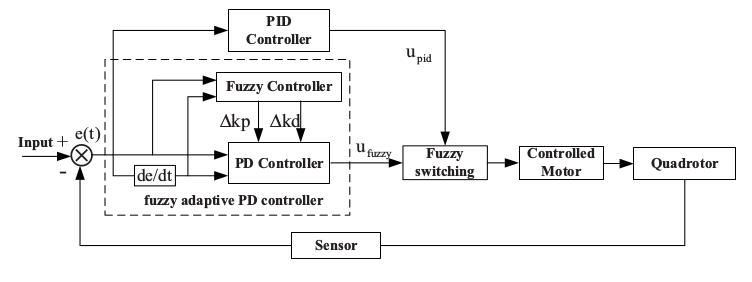
\includegraphics[width=0.9\textwidth]{./04-figuras/Gao2014Precision_block_diagram}
    \fonte{\citeonline{Gao2014Precision}}
    \label{fig:Gao2014Precision_block_diagram}
\end{figure}

Em relação à estrutura fuzzy, mais uma vez aqui há duas entradas para a inferência: o erro, sua derivada e os conjuntos fuzzy para cada uma delas consistem de sete variáveis linguísticas: $e$ = \{NB, NM, NS, ZO, PS, PM, PB\}, $e_c$ = \{NB, NM, NS, ZO, PS, PM, PB\}. A variável de saída do sistema Fuzzy PD é apenas uma: $U_{fuzzy}$ = \{ZO, PS, PM, PB\}. O \autoref{qua:Gao2014Precision_table_rules_inference} mostra as regras definidas para o sistema de inferência fuzzy.

\begin{quadro}[!htb]
    \centering
    \caption{Regras de inferência fuzzy usadas em \cite{Gao2014Precision}\label{qua:Gao2014Precision_table_rules_inference}}
    \begin{tabular}{c|c|c|c|c|c|c|c|}
        \cline{2-8}
        & \multicolumn{7}{c|}{\textbf{$\Delta E_c$}} \\
        
        %cabeçalho
        \hline
        \multicolumn{1}{ |c| }{\textbf{E}} & 
                            \textbf{NB} &
                            \textbf{NN} & 
                            \textbf{NS} & 
                            \textbf{ZO} & 
                            \textbf{PS} & 
                            \textbf{PM} & 
                            \textbf{PB} \\
        \hline
        %NB OK
        \multicolumn{1}{ |c| }{\textbf{NB}} & 
                            PB &
                            PM &
                            PM &
                            PS &
                            PM &
                            PM &
                            PB \\
        \hline
        %NM OK
        \multicolumn{1}{ |c| }{\textbf{NM}} & 
                            PB &
                            ZO &
                            ZO &
                            PS &
                            ZO &
                            ZO &
                            ZO \\
        \hline
        %NS OK
        \multicolumn{1}{ |c| }{\textbf{NS}} & 
                            ZO &
                            ZO &
                            PS &
                            ZO &
                            PM &
                            PB &
                            ZO \\
        \hline
        %ZO OK
        \multicolumn{1}{ |c| }{\textbf{ZO}} & 
                            PM &
                            PB &
                            PS &
                            ZO &
                            ZO &
                            PM &
                            PB \\
        \hline
        %PS OK
        \multicolumn{1}{ |c| }{\textbf{PS}} & 
                            PS &
                            PB &
                            PS &
                            PM &
                            PS &
                            ZO &
                            PB \\
        \hline
        %PM 
        \multicolumn{1}{ |c| }{\textbf{PM}} & 
                            PB &
                            ZO &
                            ZO &
                            PM &
                            ZO &
                            PM &
                            ZO \\
        \hline
        %PB 
        \multicolumn{1}{ |c| }{\textbf{PB}} & 
                            ZO &
                            PM &
                            PM &
                            ZO &
                            PM &
                            PM &
                            PM \\
        \hline
    \end{tabular}
    \fonte{Adaptado de \citeonline{Gao2014Precision}}
\end{quadro}







O controlador Fuzzy PD é adotado para garantir uma supressão rápida e com sobrelevação quando o desvio é grande. Já o controlador PID é adotado para eliminar o estado estacionário quando o desvio é pequeno.

A definição de qual dos controles irá atuar, depende do bloco \textit{Fuzzy switching}, que avalia os sinais $u_{pid}$ e $u_{fuzzy}$, e utiliza o mais apropriado entre eles. A regra utilizada é a seguinte: se $E(k)$ é $SE$ e $\Delta EC(k)$ é $S\Delta EC$ então $U$ é $U_{pid}$, senão $U$ é $U_{fuzzy}$, em que $U_{fuzzy}$ e $U_{pid}$ são as saídas dos controladores Fuzzy PD e PID respectivamente. $SE$ e $S\Delta EC$ são, respectivamente, funções de pertinência fuzzy das variáveis $E$ e $\Delta E_c$.

Nas simulações feitas, foram comparados três controladores diferentes: \textit{Backstepping}, PID e Fuzzy PD. Foi verificado que, embora o controlador \textit{Backstepping} seja pior que os outros dois, ele pode rapidamente suprimir o impacto de perturbações. Foi mostrado ainda que o controlador Fuzzy PD obteve o melhor resultado relacionado a rejeição de perturbações. O tempo de subida do controlador Fuzzy PD é ligeiramente menor nos eixos x e z mas um pouco maior no eixo y. Após numerosas simulações, verificou-se que o controlador proposto é, de fato, eficaz para manter a estabilidade de um helicóptero quadrotor.

%15
%\cite{Fatan2013}
%\citeonline{Fatan2013} propuseram, para o controle de estabilidade de um \textit{drone}, um ANP (\textit{Adaptive Neuro PID Controller}\footnote{Controlador Neuro PID Adaptativo}), que na verdade não implementa de fato uma rede neural. O nome foi dado devido à similaridade de estrutura entre o controlador obtido e uma rede neural, em que o sistema atua, no treinamento, para ajustar os pesos das conexões. O controlador implementado utiliza outra técnica de IA: é utilizado um algoritmo genético para ajustar três pesos $w_1$, $w_2$ e $w_3$, responsáveis por ajustar os pesos $\Delta K_p$, $\Delta K_i$ e $\Delta K_d$ do controlador PID respectivamente.
%
%A importante vantagem deste método é não precisar de análises matemáticas para cada situação de perturbação a ser enfrentada pelo \textit{drone} sendo ele próprio capaz de ajustar os pesos para que o controle seja efetivo em diferentes condições. Entretanto, não é garantido que os coeficientes apropriados sejam obtidos para todos os casos. Outro problema é a questão de o fator de aprendizagem utilizado no controlador ser crítica, uma vez que uma taxa muito baixa pode não levar a uma adaptação rápida o suficiente para garantir a estabilidade numa mudança de situação. Apesar das limitações, foi mostrado que o controlador ANP pode controlar o sistema na presença de ruídos e perturbações que mesmo o controlador PID com ganhos bem definidos não pode controlar bem.

%17
%\cite{Yacef2013}
Outras abordagens híbridas ainda foram adotadas para o projeto de controladores de estabilidade para \textit{drones}. Em \cite{Yacef2013}, foi proposto o uso do PSO para ajuste de um IBC. O método é usado para minimizar o erro quadrático (SE) de uma função de custo que quantifica a performance de todo o sistema. Resultados de numerosas simulações mostram a validação e as boas performances alcançadas pelo método proposto.

%18
%\cite{Boubertakh2013}
Em \cite{Boubertakh2013} é proposta uma ideia parecida: utilizar o algoritmo PSO para ajustar os pesos de quatro controladores PD, cada qual responsável por controlar um rotor. A ideia é usar o PSO para minimizar o SE da função de custo que quantifica o sistema, assim como visto em \cite{Yacef2013}. As simulações feitas mostraram a eficácia do controlador proposto.

Como se pode ver, as técnicas inteligentes têm sido largamente utilizadas para propor diferentes tipos de controladores para quadrotores. Como já dito anteriormente, isso deve às inúmeras vantagens citadas que elas trazem. Algumas dessas técnicas foram utilizadas neste trabalho, como é mostrado a seguir.

%\section{Controle de Estabilidade de Helicópteros Quadrotores}
%\label{sec:trab-rel-quadrotores}
%
%Há também inúmeros trabalhos relacionados ao controle de estabilidade de quadrotores a partir dos mais diversos métodos. Os trabalhos propõem controladores usando métodos tradicionais de controle (e.g.\ PD, PID, LQR), métodos de Inteligência Artificial/ Inteligência Computacional (e.g.\ Fuzzy, Neuro-Fuzzy, PSO) ou, ainda, métodos híbridos, combinando elementos do controle tradicional às técnicas de controle inteligente.
     % Trabalhos relacionados
%    %
% Documento: Metodologia
%

\chapter{Metodologia}
\label{chap:metodologia}

Em ambiente simulado, utilizando a modelagem computacional de um quadrotor com desacoplamento das entradas proposto por \citeonline{Balas2007} e mostrado na seção \ref{sec:sistemas-nao-lineares-quadrotor}, foram propostos, para estabilizar o sistema, controladores aplicando duas técnicas diferentes de IC: fuzzy e neuro-fuzzy. Todas as simulações e execuções se deram utilizando a versão R2015a do MATLAB.

\section{Controladores Fuzzy}
\label{sec:controlador-fuzzy}

O projeto dos controlador fuzzy foi focado na estabilização de atitude e altitude de um drone sujeito a parâmetros específicos\footnote{Estes valores foram também utilizados por \citeonline{Balas2007} para definir uma especificação do sistema}, sendo eles: a gravidade $g=9,81$ $m/s^2$, a massa do quadrotor $m=2,3$ $kg$ e o comprimento de cada haste do drone $l=0,5$ $m$. Um dos controladores projetado tem, como objetivo, controlar a altitude do drone, ao passo que um segundo visa a estabilização de sua atitude.

O controlador de altitude possui duas entradas e uma saída. As entradas são referentes à posição vertical do quadrotor ($z$) e sua respectiva velocidade ($\dot{z}$), ao passo que a saída diz respeito ao sinal de controle a ser aplicado sobre o sistema para estabilizar sua altitude ($u_1$). Sua aplicação no sistema é mostrada na Figura \ref{fig:u1_mamdani_blocks}.

% Mostrar diagrama do sistema controlado (para ruídos), sobre a entrada u1
\begin{figure}[!htb]
    \centering
    \caption{Diagrama do sistema de controle de altitude utilizando controlador fuzzy}
    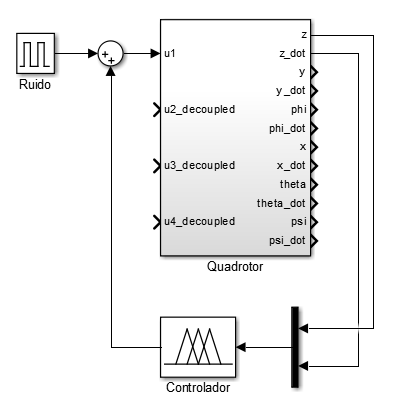
\includegraphics[width=0.5\textwidth]{./04-figuras/resultados/novos/simulink_printscreen_z}
    \label{fig:u1_mamdani_blocks}
\end{figure}

Utilizando o \textit{Fuzzy Logic Toolbox} do MATLAB, cada variável linguística do controlador fuzzy foi divida em três conjuntos: N (negativo), Z (zero) e P (positivo), baseado nos trabalhos de \citeonline{Maj2013} e \citeonline{Gao2014Stability}. As regras fuzzy definidas para este controlador são mostradas no Quadro \ref{qua:regras_fuzzy_u1_mamdani}, e a Figura \ref{fig:1_mamdani_surface} exibe seu equivalente em superfície.

% Mostrar regras Fuzzy envolvidas no controle de u1 (quadro de regras + superfície)
% Tá errada!
\begin{quadro}[!htb]
    \centering
    \caption{Regras fuzzy para modelagem do controle de altitude\label{qua:regras_fuzzy_u1_mamdani}}
    \begin{tabular}{|c|c|c|}
    % \begin{tabular}{>{\centering\bfseries}m{1in} >{\centering}m{1in}
        \hline
        \textbf{{$z$}} & 
        \textbf{{$\dot{z}$}} &
        \textbf{{$u_1$}} \\
        \hline %01
            N &
            - &
            N \\
        \hline %02
            P &
            - &
            P \\
        \hline %03
            Z &
            N &
            N \\
        \hline %04
            Z &
            Z &
            Z \\
        \hline %05
            Z &
            P &
            P \\
        \hline
    \end{tabular}
    % \begin{TAB}(r,1cm,2cm)[5pt]{|c|c|}{|c|c|c|}% (rows,min,max)[tabcolsep]{columns}{rows}
    %     hi & tall one    \\
    %     hi & medium one  \\
    %     hi & standard one\\
    % \end{TAB}
\end{quadro}


\begin{figure}[!htb]
    \centering
    \caption{Superfície das regras do sistema de controle fuzzy para a altitude do quadrotor}
    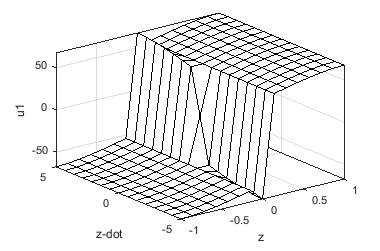
\includegraphics[width=0.6\textwidth]{./04-figuras/resultados/fis_u1/u1_mamdani_surface}
    \label{fig:1_mamdani_surface}
\end{figure}

O controlador de atitude projetado também possui duas entradas e uma saída. Desta vez, entretanto, as entradas são referentes ao ângulo em relação ao eixo horizontal ($\phi$ ou $\theta$) e sua respectiva variação ($\dot{\phi}$ ou $\dot{\theta}$). Mais uma vez, cada variável linguística foi dividida em três conjuntos: N, Z e P.

As regras que regem o controlador de atitude são sintetizadas no Quadro \ref{qua:regras_fuzzy_u2_u3_mamdani} e podem ser vistas na superfície de regras mostradas na Figura \ref{fig:u2_u3_mamdani_surface}.

% Mostrar regras Fuzzy envolvidas no controle de u2 e u3 (quadro de regras + superfície)
\begin{quadro}[!htb]
    \centering
    \caption{Regras fuzzy para modelagem do controle de atitude\label{qua:regras_fuzzy_u2_u3_mamdani}}
    \begin{tabular}{|c|c|c|}
    % \begin{tabular}{>{\centering\bfseries}m{1in} >{\centering}m{1in}
        \hline
        \textbf{{$\phi/\theta$}} & 
        \textbf{{$\dot{\phi}/\dot{\theta}$}} &
        \textbf{{$u_2/u_3$}} \\
        \hline %01
            P &
            P &
            N \\
        \hline %02
            P &
            Z &
            N \\
        \hline %03
            P &
            N &
            Z \\
        \hline %04
            N &
            N &
            P \\
        \hline %05
            N &
            Z &
            P \\
        \hline %06
            N &
            P &
            Z \\
        \hline %07
            Z &
            Z &
            Z \\
        \hline %08
            Z &
            N &
            P \\
        \hline %09
            Z &
            P &
            N \\
        \hline
    \end{tabular}
    % \begin{TAB}(r,1cm,2cm)[5pt]{|c|c|}{|c|c|c|}% (rows,min,max)[tabcolsep]{columns}{rows}
    %     hi & tall one    \\
    %     hi & medium one  \\
    %     hi & standard one\\
    % \end{TAB}
\end{quadro}


\begin{figure}[!htb]
    \centering
    \caption{Superfície das regras do sistema de controle fuzzy para a atitude do quadrotor}
    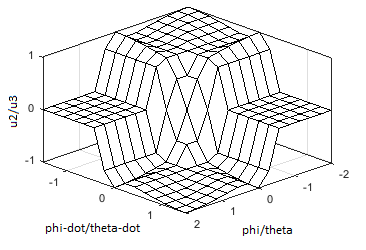
\includegraphics[width=0.6\textwidth]{./04-figuras/resultados/fis_u2/u2_u3_mamdani_surface}
    \label{fig:u2_u3_mamdani_surface}
\end{figure}

Já as Figuras \ref{fig:u2_mamdani_blocks} e \ref{fig:u3_mamdani_blocks} exibem os diagramas do sistema controlado, com atuação sobre os ângulos $\phi$ e $\theta$, respectivamente.

% Mostrar diagrama do sistema controlado (para ruídos), sobre as entradas u2 e u3
\begin{figure}[!htb]
    \centering
    \caption{Diagrama do sistema de controle de atitude utilizando controlador fuzzy sobre o ângulo $\phi$}
    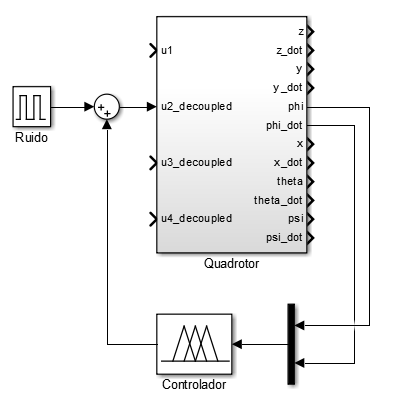
\includegraphics[width=0.6\textwidth]{./04-figuras/resultados/novos/simulink_printscreen_phi}
    \label{fig:u2_mamdani_blocks}
\end{figure}

\begin{figure}[!htb]
    \centering
    \caption{Diagrama do sistema de controle de atitude utilizando controlador fuzzy sobre o ângulo $\theta$}
    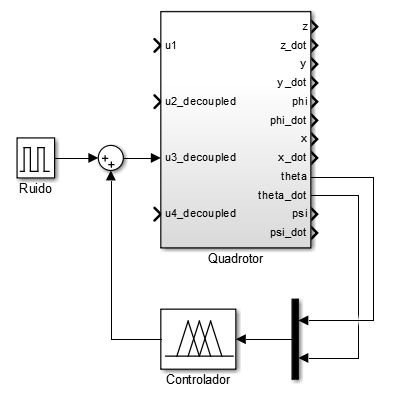
\includegraphics[width=0.5\textwidth]{./04-figuras/resultados/novos/simulink_printscreen_theta}
    \label{fig:u3_mamdani_blocks}
\end{figure}









\section{Controladores Neuro-Fuzzy}
\label{sec:controlador-neuro-fuzzy}

A partir dos controladores de atitude e altitude fuzzy projetados, foram propostos dois controladores do tipo neuro-fuzzy: um para cada dos casos.

Para tanto, foram utilizados os códigos mostrados nos Apêndices \ref{chap:train-anfis-altitude} e \ref{chap:train-anfis-atitude}. No processo de criação do controlador de altitude neuro-fuzzy, foram gerados trezentos\footnote{Este valor foi arbitrado por corresponder a uma quantidade razoável para treinar a RNA sem que se alcance o sobreajuste, conhecido como \textit{overfitting}} pares de entradas e cada um deles foi submetido ao processo de inferência fuzzy utilizando o controlador previamente modelado. Dois terços desses dados foram utilizados para gerar o conjunto de treinamento, representado pela variável {\ttfamily train} e o um terço restante foi armazenado na variável {\ttfamily test} e utilizado para validação do treinamento. Então, utilizando o comando {\ttfamily mam2sug} do MATLAB, foi gerado um modelo fuzzy Sugeno a partir do Mamdani que havia sido modelado e este novo arquivo foi salvo sob o nome {\ttfamily fis\_altitude\_neuro.fis}.

Feito isto, utilizou-se o comando comando {\ttfamily anfisedit} para abrir o \textit{Neuro-Fuzzy Designer} do MATLAB, cuja interface é mostrada na Figura \ref{fig:anfisedit_screen}. No campo marcado pelo número 2 na imagem (\textit{Generate FIS}), clicou-se no botão \textit{Load} e se selecionou o arquivo {\ttfamily fis\_altitude\_neuro.fis} que fora gerado pelo código executado. Após isto, no campo marcado pelo número 1 (\textit{Load Data}), marcou-se \textit{Training} e \textit{worksp} para utilizar uma variável da área de trabalho do MATLAB para treinar a rede. Após clicar em \textit{Load Data}, digitou-se {\ttfamily train}, nome da variável definida no código. Então, no campo marcado pelo número 3, marcou-se \textit{Training Data} e se clicou no botão \textit{Test Now} para executar o treinamento da rede. Após estes passos, a rede neuro-fuzzy foi devidamente treinada e sua estrutura, mostrada na Figura \ref{fig:rna_anfis_altitude_gray}, pode ser obtida clicando no botão \textit{Structure} logo acima do campo 3. Esta estrutura relaciona as variáveis de entrada e suas funções de pertinência, através das regras fuzzy, à saída do sistema e às suas funções de pertinência, em que cada componente representa um neurônio da RNA obtida. 

\begin{figure}[!htb]
    \centering
    \caption{Interface gráfica da ferramenta \textit{Neuro-Fuzzy Designer} com destaque aos três campos necessários para treinamento e teste da rede neuro-fuzzy}
    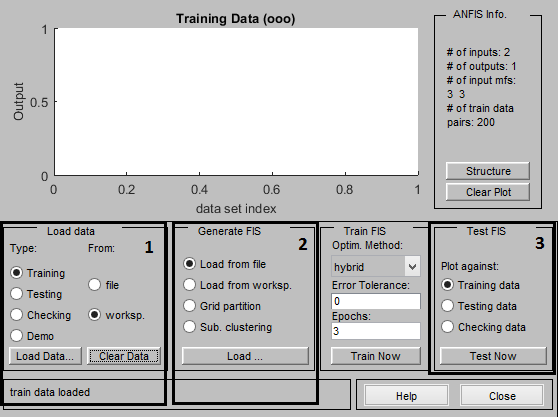
\includegraphics[width=0.8\textwidth]{./04-figuras/anfisedit/anfisedit_screen}
    \label{fig:anfisedit_screen}
\end{figure}

\begin{figure}[!htb]
    \centering
    \caption{Diagrama da RNA referente ao controlador neuro-fuzzy para altitude}
    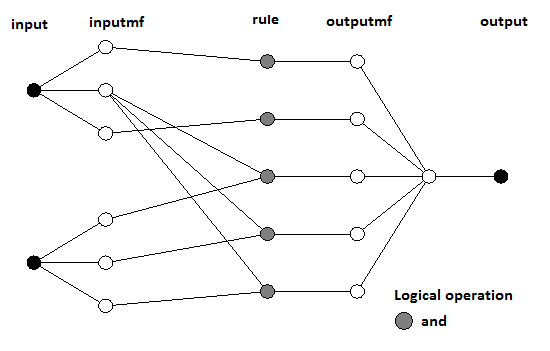
\includegraphics[width=0.6\textwidth]{./04-figuras/anfisedit/rna_anfis_altitude_gray}
    \label{fig:rna_anfis_altitude_gray}
\end{figure}

Após o término do treinamento, deve-se submeter a rede ao processo de treinamento. Para tanto, basta selecionar \textit{Testing} no campo marcado pelo número 1, deixar marcada a opção \textit{worksp}, clicar no botão \textit{Load Data} e escolher a variável {\ttfamily test}, que também foi definida no código executado.

A Figura \ref{fig:rna_anfis_train_result_altitude} mostra o gráfico obtido na ferramenta após o processo de treinamento, em que os círculos brancos mostram os dados utilizados no treinamento e os asteriscos pretos indicam o valor referentes a eles obtidos pela rede treinada.

\begin{figure}[!htb]
    \centering
    \caption{Resultado obtido pelo treinamento da RNA para controle de altitude}
    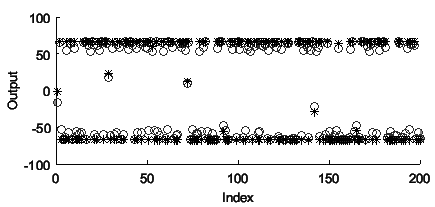
\includegraphics[width=0.6\textwidth]{./04-figuras/anfisedit/rna_anfis_train_result_altitude}
    \label{fig:rna_anfis_train_result_altitude}
\end{figure}

%Feito isto, após utilizar o comando {\ttfamily anfisedit} para abrir o \textit{Neuro-Fuzzy Designer} do MATLAB, carregou-se, nesta ferramenta, o arquivo {\ttfamily fis\_altitude\_neuro.fis} como sistema a ser treinado e, utilizando as variáveis {\ttfamily train} e {\ttfamily test}, o sistema foi devidamente treinado e validado. Após este processo, obteve-se um controlador neuro-fuzzy cujo funcionamento é mostrado pela superfície de regras mostradas na Figura \ref{fig:u1_sugeno_surface}.

Um processo similar foi aplicado para modelar o controlador de atitude neuro-fuzzy, como mostra o Apêndice \ref{chap:train-anfis-atitude}. As Figuras \ref{fig:rna_anfis_atitude_gray} e \ref{fig:rna_anfis_train_result_atitude} mostram o diagrama da RNA referente ao controlador neuro-fuzzy para atitude e o resultado obtido pelo seu treinamento respectivamente.

\begin{figure}[!htb]
    \centering
    \caption{Diagrama da RNA referente ao controlador neuro-fuzzy para atitude}
    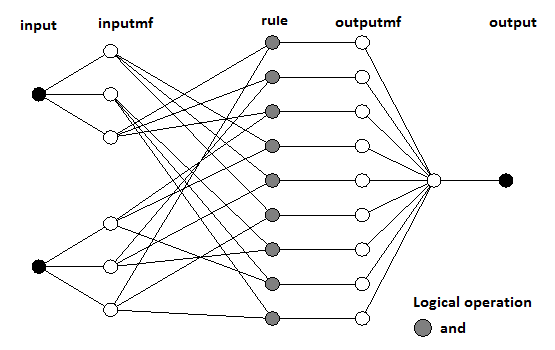
\includegraphics[width=0.6\textwidth]{./04-figuras/anfisedit/rna_anfis_atitude_gray}
    \label{fig:rna_anfis_atitude_gray}
\end{figure}

\begin{figure}[!htb]
    \centering
    \caption{Resultado obtido pelo treinamento da RNA para controle de atitude}
    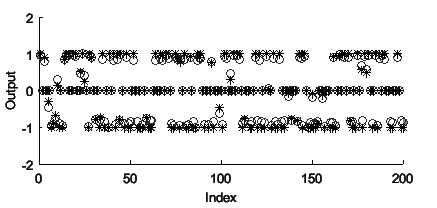
\includegraphics[width=0.6\textwidth]{./04-figuras/anfisedit/rna_anfis_train_result_atitude}
    \label{fig:rna_anfis_train_result_atitude}
\end{figure}

O processo de treinamento determina o comportamento dos controladores neuro-fuzzy projetados, cujas superfícies de regras são exibidas nas Figuras \ref{fig:u1_sugeno_surface} e \ref{fig:u2_u3_sugeno_surface}.

%-----
%Utilizando o comando {\ttfamily mam2sug} do MATLAB, obteve-se um novo modelo fuzzy do tipo Sugeno para cada modelo previamente definidos: um para controle de altitude e um segundo para controle de atitude do quadrotor. Então, utilizando o \textit{Neuro-Fuzzy Designer} do MATLAB, cada um dos modelos Sugeno criados foi treinado a partir de resultados obtidos pelos modelos fuzzy previamente elaborados. Não houve nenhuma alteração nas regras dos sistema, mas, devido às generalizações e aprendizagem da rede neuro-fuzzy, a relação entre valores de cada conjunto de saída foi ligeiramente alterado. Isso pode ser visto a partir das superfícies de regras para ambos os controladores, mostradas nas Figuras \ref{fig:u1_sugeno_surface} e \ref{fig:u2_u3_sugeno_surface}.

% Mostrar superfície Sugeno
\begin{figure}[!htb]
    \centering
    \caption{Superfície das regras do sistema de controle neuro-fuzzy para a altitude do quadrotor}
    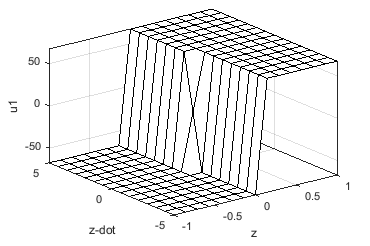
\includegraphics[width=0.6\textwidth]{./04-figuras/resultados/fis_u1/u1_sugeno_surface}
    \label{fig:u1_sugeno_surface}
\end{figure}

\begin{figure}[!htb]
    \centering
    \caption{Superfície das regras do sistema de controle fuzzy para a atitude do quadrotor}
    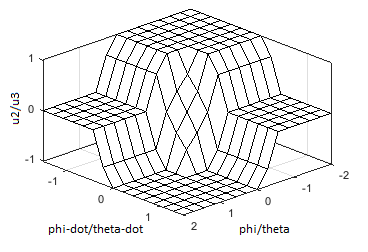
\includegraphics[width=0.6\textwidth]{./04-figuras/resultados/fis_u3/u2_u3_sugeno_surface}
    \label{fig:u2_u3_sugeno_surface}
\end{figure}




\section{Experimentos Realizados}
\label{sec:experimentos-realizados}

O primeiro experimento feito foi para mostrar a instabilidade do sistema, mostrando a resposta das variáveis relacionadas à atitude (ângulos $\phi$ e $\theta$) e altitude ($z$) quando o sistema é submetido a um breve impulso em suas entradas, simulando qualquer força que possa atuar brevemente sobre o quadrotor, como um golpe sofrido por qualquer objeto que colida com ele. Após contextualizada a necessidade de controladores, passou-se à sua implementação e uso.

Uma vez projetados os controladores fuzzy e neuro-fuzzy, o sistema foi sujeitado a distúrbios em atitude e altitude para verificar o funcionamento deles sob condições similares às mostradas quando nenhum controle agia sobre ele fazendo com que o sistema divergisse.. Primeiramente, o comportamento de ambos os controladores foi verificado quando atuando sobre o sistema para os quais eles foram projetados, com $g=9,81$ $m/s^2$, $m=2,3$ $kg$ e $l=0,5$ $m$. 

Em seguida, para testar a robustez de cada controlador, foi feita uma simulação em que eles atuam sobre um sistema cuja massa do quadrotor é $m=5$ $kg$, valor este que foi escolhido por variar o parâmetro massa em mais de 100 \%.

Os resultados obtidos são mostrados no capítulo seguinte.


%
%O desenvolvimento do trabalho se deu integralmente em ambiente simulado. Para a implementação das simulações, foi utilizado o software MATLAB\textregistered, devido à grande gama de possibilidades que ele oferece para lidar com sistemas não lineares além do excelente material de apoio da própria MathWorks\textregistered\ e da comunidade de usuários. As ferramentas do MATLAB utilizadas foram:
%\begin{itemize}
%  \item Simulink: utilizado para modelar sistemas em diagramas de blocos e fazer simulações dos sistemas resultantes;
%  \item Fuzzy Logic Toolbox: utilizado para desenvolver controladores Fuzzy.
%  \item Neuro-Fuzzy Designer: utilizado para treinar e validar controladores Neuro-Fuzzy.
%\end{itemize}
%
%\section{Contextualização do Controle de Sistemas Dinâmicos Não Lineares}
%\label{sec:metodologia-contextualizacao}
%
%Para a contextualização da ação de controle sobre sistemas não lineares, escolheu-se o sistema de pêndulo invertido por ser análogo ao modelo do \textit{drone}. Esta escolha foi baseada no fato de este sistema ser considerado um problema clássico de sistema não linear instável, sendo retratado repetidamente na literatura, como em \cite[p.~68]{Ogata2010} e em \cite[p.~186]{Dorf2011}, além de ser largamente usado como \textit{benchmark} para comparação de eficiência de variados métodos de controle, sendo alvo de estudo em diversos artigos. O primeiro passo para seu estudo é a sua modelagem matemática.

\subsection{Modelagem Matemática}
\label{subsec:sistemas-pendulum-mathematical-model}

Considerando o diagrama de corpo livre mostrado na \autoref{fig:Ogata2010_inverted_pendulum_diagram_complete}-b e se utilizando de desenvolvimento matemático chegou-se às seguintes equações para descrever o movimento do sistema do pêndulo invertido sobre o carro:
\begin{equation} \label{eq:modeling_pendulum_eq1}
	(M+m)\ddot{x} + ml\ddot{\theta} = u
\end{equation}
\begin{equation} \label{eq:modeling_pendulum_eq2}
	(I+ml^2)\ddot{\theta} + ml\ddot{x} = mlg\theta
\end{equation}
 
Em que $I$ é o momento de inércia da haste.

A partir de manipulação matemática, as equações \ref{eq:modeling_pendulum_eq1} e \ref{eq:modeling_pendulum_eq2} podem ser reescritas como:
\begin{equation} \label{eq:modeling_pendulum_eq1_modified}
	Ml\ddot{\theta} = (M+m)g\theta - u
\end{equation}
\begin{equation} \label{eq:modeling_pendulum_eq2_modified}
	M\ddot{x} = u - mg\theta
\end{equation}

A partir da \autoref{eq:modeling_pendulum_eq2_modified}, \citeonline[p.~71]{Ogata2010} obtém a função de transferência da planta como:
\begin{align} \label{eq:modeling_pendulum_tf}
\frac{\Theta(s)}{-U(s)} &= \frac{1}{Mls^2-(M+m)g} \nonumber \\
						&= \frac{1}{Ml(s+\sqrt{\frac{M+m}{Ml}g})(s-\sqrt{\frac{M+m}{Ml}g})}
\end{align}

Na \autoref{eq:modeling_pendulum_tf}, verifica-se que a planta do pêndulo invertido possui um polo no eixo real negativo e outro no eixo real positivo. Estes polos são: 
\begin{equation} \label{eq:modeling_pendulum_tf_neg_pole}
	s = -\sqrt{\frac{M+m}{Ml}g}
\end{equation}
\begin{equation} \label{eq:modeling_pendulum_tf_pos_pole}
	s = \sqrt{\frac{M+m}{Ml}g}
\end{equation}

Por possuir um polo no eixo real positivo, definido pela \autoref{eq:modeling_pendulum_tf_pos_pole}, a planta é instável em malha aberta.

\subsection{Representação no Espaço de Estados}
\label{subsec:sistemas-inverted-pendulum-state-spaces}
Para a representação do sistema no espaço de estados, em \cite[p.~71]{Ogata2010} as variáveis de estado $x_1$, $x_2$, $x_3$ e $x_4$ foram definidas como:
\begin{align*}
	x_1 &= \theta \\
	x_2 &= \dot{\theta} \\
	x_3 &= x \\
	x_4 &= \dot{x}
\end{align*}

Com isto, se obtém o vetor de estados $X$ definido por:
\begin{equation*}
X=
\left[ \begin{array}{@{}*{4}{c}@{}}
     \theta & \dot{\theta} & x & \dot{x} \\
\end{array} \right]^T
\end{equation*}

Além disto, o vetor $y$ de saída do sistema foi definido como:
\[
	y = 
	\begin{bmatrix}
		y_1 \\
		y_2
	\end{bmatrix} = 
	\begin{bmatrix}
			\theta \\
			x
	\end{bmatrix} =
	\begin{bmatrix}
			x_1\\
			x_3
	\end{bmatrix}
\]

A partir de novas manipulações matemáticas, mostra-se que a representação por espaço de estados deste sistema de pêndulo invertido pode ser definido como:
\begin{align} \label{eq:space_state_equation_pendulum}
	\dot{x} &= Ax + Bu \\
	y		&= Cx + Du
\end{align}

Em que:
\[
	A = 
	\begin{bmatrix}
		0 & 1 & 0 & 0 \\
		\frac{M+m}{Ml}g & 0 & 0 & 0 \\
		0 & 0 & 0 & 1 \\
		-\frac{m}{M}g & 0 & 0 & 0
	\end{bmatrix}\quad
	B = 
	\begin{bmatrix}
		0 \\
		-\frac{1}{Ml} \\
		0 \\
		\frac{1}{Ml}
	\end{bmatrix}
\]

\[
	C = 
		\begin{bmatrix}
			1 & 0 & 0 & 0 \\
			0 & 0 & 1 & 0
		\end{bmatrix}\quad
	D = 
		\begin{bmatrix}
			0 \\
			0
		\end{bmatrix}
\]

Desta forma, se obtém a representação completa do sistema de pêndulo invertido no espaço de estados.

\subsection{Experimentos Realizados}
\label{subsec:metodolgoia-pendulum-experimentos}

Uma variação do algoritmo presente em \cite[p.~750]{Ogata2010} foi usado para simular a resposta do sistema de pêndulo invertido a uma entrada em degrau unitário em duas situações: sem nenhuma ação de controle; e com uma ação de controle tradicional. Neste segundo caso, foi utilizado um servo sistema tipo 1, como mostrado na \autoref{fig:Ogata2010_servo_system_type_1}.

\begin{figure}[!htb]
    \centering
    \caption{Diagrama de blocos representando o sistema de pêndulo invertido controlado por um servo sistema tipo 1}
    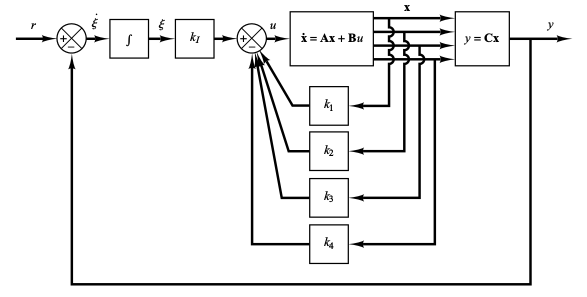
\includegraphics[width=1\textwidth]{./04-figuras/Ogata2010_servo_system_type_1}
    \fonte{\cite[p.~747]{Ogata2010}}
    \label{fig:Ogata2010_servo_system_type_1}
\end{figure}

Os parâmetros do controlador utilizados foram \cite[p.~749]{Ogata2010}:
\[
	k = 
		\begin{bmatrix}
			k_1 &
			k_2 &
			k_3 &
			k_4
		\end{bmatrix} =
		\begin{bmatrix}
			-157,6336 &
			-35,3733 &
			-56,0652 &
			50,9684
		\end{bmatrix}
\]

e
\[
k_I = -50,9684
\]

O algoritmo que implementa o sistema do pêndulo invertido e também o controlador proposto é mostrado no Apêndice \ref{chap:apendicex-pendulum-modelagem-controle}. O intuito desta etapa é mostrar a instabilidade do sistema, que diverge ao sofrer qualquer perturbação, e a ação de controle que estabiliza este sistema, tornando-o estável, fazendo com que ele não mais divirja quando perturbado.

O diagrama de blocos do sistema desenvolvido para representar o pêndulo invertido é mostrado na \autoref{fig:simulink-pendulo-diagrama-geral}. Como se pode ver, este sistema possui uma única entrada, $u$, referente à força aplicada sobre o carro, e quatro saídas: theta ($\theta$) representando o ângulo da haste do pêndulo em relação ao eixo vertical; theta\_dot ($\dot{\theta}$), a taxa de variação deste ângulo; x, a posição do carro sobre o eixo horizontal; e x\_ponto ($\dot{x}$), sua velocidade sobre este mesmo eixo.

\begin{figure}[!htb]
    \centering
    \caption{Diagrama de blocos representando o sistema de pêndulo invertido}
    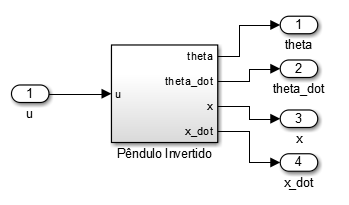
\includegraphics[width=.6\textwidth]{./04-figuras/simulink_pendulo/diagrama_geral}
    \label{fig:simulink-pendulo-diagrama-geral}
\end{figure}

A estrutura do primeiro experimento realizado é mostrado na \autoref{fig:simulink-pendulo-diagrama-geral-step}. Como se pode ver, foi aplicada à entrada $u$ do sistema, uma entrada em degrau unitário. Neste experimento, são verificadas as resposta de todas as saídas a esta excitação na entrada. Para permitir uma clara distinção da resposta do sistema sem a excitação e com ela, foi definido que ela ocorresse no tempo $t=10\ s$.

\begin{figure}[!htb]
    \centering
    \caption{Diagrama de blocos representando experimento realizado com o sistema de pêndulo invertido}
    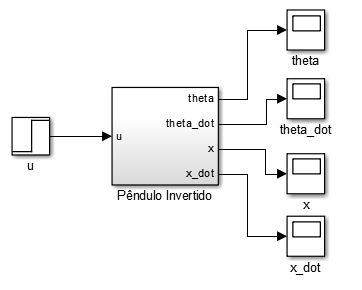
\includegraphics[width=.6\textwidth]{./04-figuras/simulink_pendulo/diagrama_step_u}
    \label{fig:simulink-pendulo-diagrama-geral-step}
\end{figure}

A estrutura do segundo experimento é análoga à do primeiro. Uma excitação em degrau é aplicada na entrada e todos os estados são verificados. Para este experimento, entretanto, a estrutura inclui um servo sistema tipo um, como mostrado na \autoref{fig:Ogata2010_servo_system_type_1},  para estabilizar o pêndulo.

%
%\section{Modelagem e Controle do Quadrotor}
%\label{sec:metodologia-quadcopter}
%
%A modelagem matemática utilizada para um quadrotor neste trabalho foi a proposta por \citeonline{Balas2007}, devido à sua abordagem completa incluindo diferentes estágios: desacoplamento das entradas, dinâmicas dos rotores e modelagem do quadrotor em si. A estrutura utilizada nesta modelagem é mostrada na \autoref{fig:Balas2007_diagram_blocos_drone_abordagem_engenharia}.

\begin{figure}[!htb]
    \centering
    \caption{Diagrama de blocos do sistema de representação de um quadricóptero}
    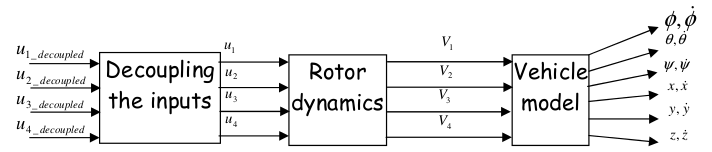
\includegraphics[width=1\textwidth]{./04-figuras/Balas2007_diagram_blocos_drone_abordagem_engenharia}
    \fonte{\citeonline[p.~58]{Balas2007}}
    \label{fig:Balas2007_diagram_blocos_drone_abordagem_engenharia}
\end{figure}

Nesta estrutura, $u_1$ representa o empuxo total sobre o quadricóptero, $u_2$ representa o momento de \textit{roll} (em torno do eixo $x$), $u_3$ representa o momento de \textit{pitch} (em torno do eixo $y$) e $u_4$ representa o momento de \textit{yaw} (em torno do eixo $z$). $u_{2\textunderscore decoupled}$, $u_{3\textunderscore decoupled}$ e $u_{4\textunderscore decoupled}$ são combinações de $u_2$, $u_3$ e $u_4$ de tal forma que as entradas $u_{2\textunderscore decoupled}$, $u_{3\textunderscore decoupled}$ e $u_{4\textunderscore decoupled}$ tenham as mesmas direções que os ângulos de Euler, $\phi$, $\theta$ e $\psi$, respectivamente. A relação entre estas entradas é dada, em \cite[p.~49]{Balas2007} por:
\[
	\begin{bmatrix}
		u'_{2} \\
		u'_{3} \\
		u'_{4}
	\end{bmatrix} = 
	\begin{bmatrix}
		cos_{\psi_{0}} & sen_{\psi_{0}}cos_{\phi_{0}}\frac{I_{xx}}{I_{yy}} & 
		0 \\
		
		-sen_{\psi_{0}}\frac{I_{yy}}{I_{xx}} &
		cos_{\psi_{0}}cos_{\phi_{0}} &
		0 \\
		
		0 &
		-sen_{\phi_{0}}\frac{I_{zz}}{I_{yy}} &
		1
	\end{bmatrix}
	\begin{bmatrix}
		u'_{2\textunderscore decoupled} \\
		u'_{3\textunderscore decoupled} \\
		u'_{4\textunderscore decoupled}
	\end{bmatrix}
\]

$I_{xx}$, $I_{yy}$ e $I_{zz}$ representam o momento de inércia do quadricóptero ao longo dos eixos $x$, $y$ e $z$, respectivamente.

Na \autoref{fig:Balas2007_diagram_blocos_drone_abordagem_engenharia}, o primeiro bloco, referente ao desacoplamento das entradas, atua justamente convertendo as entradas $u_{1\textunderscore decoupled}$ $u_{2\textunderscore decoupled}$, $u_{3\textunderscore decoupled}$ e $u_{4\textunderscore decoupled}$ de forma a se obter $u_1$, $u_2$, $u_3$ e $u_4$ para que, no bloco seguinte, de dinâmicas dos rotores, as entradas sejam, de forma isolada, o empuxo total sobre o quadricóptero e os momentos de \textit{roll}, \textit{pitch} e \textit{yaw}. Neste bloco, estabelece-se uma relação entre essas quatro entradas e a tensão que deve ser aplicada a cada um dos rotores, $V_1$, $V_2$, $V_3$ e $V_4$.

Por fim, o último bloco, referente à \textit{Modelagem do Quadrotor}, apresenta o estado do quadrotor, fornecendo, como saída, os ângulos de \textit{roll}, \textit{pitch} e \textit{yaw}, a posição do quadrotor nos eixos $x$, $y$ e $z$ tal como a taxa de variação de cada uma destes ângulos e posições.

\subsection{Modelagem Matemática}
\label{subsec:sistemas-quadcopter-mathematical-model}

Em \cite{Balas2007}, a modelagem do quadricóptero foi feita em três partes: uma sendo referente ao empuxo vertical; uma segunda, aos momentos de \textit{roll} e \textit{pitch}; e uma terceira, ao momento de \textit{yaw}.

%Assumindo um quadricóptero com massa $m$ igual a 2,354 g e uma aceleração $g$ igual a 9,81 N.
A função de transferência obtida por \citeonline[p.~20]{Balas2007} para representar o empuxo vertical gerado pelos quatro rotores do quadrotor foi:
\begin{equation}
H(s) = \frac{2,105s-0,0425}{0,4895s^2+1,873s+1} N/V
\end{equation}

Já a função de transferência obtida para representar os momentos de \textit{roll} e de \textit{pitch} foi:
\begin{equation}
H(s) = l\frac{1,155s}{0,8696s^2+0,401s+1} Nm/V
\end{equation}

Por fim, a função de transferência obtida para representar o momento de \textit{yaw} foi:
\begin{equation}
H(s) = \frac{0,045}{0,314s+1} Nm/V
\end{equation}

\subsection{Representação no Espaço de Estados}
\label{subsec:sistemas-quadcopter-state-spaces}

Como mostrado em \cite[p.~63]{Balas2007}, o sistema modelado pode ser representado da seguinte forma no espaço de estados.
\begin{align} \label{eq:space_state_equation_quadcopter}
	\dot{x} &= Ax + Bu \nonumber \\
	y		&= Cx + Du
\end{align}

Com o vetor de estados $X$ sendo dado por:
\begin{equation*}
X=
\left[ \begin{array}{@{}*{12}{c}@{}}
     x & y & z & \dot{x} & \dot{y} & \dot{z} & \phi & \theta & \psi & \dot{\phi} & \dot{\theta} & \dot{\psi}\\
\end{array} \right]^T
\end{equation*}

O vetor de entrada $U$ sendo dado por:
\[ 
	U =
	\begin{bmatrix}
		u_1 & 
		u_{2\textunderscore decoupled} &
		u_{3\textunderscore decoupled} &
		u_{4\textunderscore decoupled}
	\end{bmatrix}^T
\]

As matriz A, B, C e D sendo definida como:
\begin{equation*}
A =
\left[ \begin{array}{@{}*{12}{c}@{}}
     0 & 0 & 0 & 1 & 0 & 0 & 0 & 0  & 0 & 0 & 0 & 0 \\
     0 & 0 & 0 & 0 & 1 & 0 & 0 & 0  & 0 & 0 & 0 & 0 \\
     0 & 0 & 0 & 0 & 0 & 1 & 0 & 0  & 0 & 0 & 0 & 0 \\
     0 & 0 & 0 & 0 & 0 & 0 & 0 & -g & 0 & 0 & 0 & 0 \\
     0 & 0 & 0 & 0 & 0 & 0 & g & 0  & 0 & 0 & 0 & 0 \\
     0 & 0 & 0 & 0 & 0 & 0 & 0 & 0  & 0 & 0 & 0 & 0 \\
     0 & 0 & 0 & 0 & 0 & 0 & 0 & 0  & 0 & 1 & 0 & 0 \\
     0 & 0 & 0 & 0 & 0 & 0 & 0 & 0  & 0 & 0 & 1 & 0 \\
     0 & 0 & 0 & 0 & 0 & 0 & 0 & 0  & 0 & 0 & 0 & 1 \\
     0 & 0 & 0 & 0 & 0 & 0 & 0 & 0  & 0 & 0 & 0 & 0 \\
     0 & 0 & 0 & 0 & 0 & 0 & 0 & 0  & 0 & 0 & 0 & 0 \\
     0 & 0 & 0 & 0 & 0 & 0 & 0 & 0  & 0 & 0 & 0 & 0 \\
\end{array}\right]
\end{equation*}

\begin{equation*}
B =
\left[\begin{array}{@{}*{4}{c}@{}}
	0 & 0 & 0 & 0 \\
	0 & 0 & 0 & 0 \\
	0 & 0 & 0 & 0 \\
	0 & 0 & 0 & 0 \\
	0 & 0 & 0 & 0 \\
	-1/m & 0 & 0 & 0 \\
	0 & 0 & 0 & 0 \\
	0 & 0 & 0 & 0 \\
	0 & 0 & 0 & 0 \\
	0 & cos(\psi)/I_{xx} & -sen(\psi)/I_{yy} & 0 \\
	0 & sen(\psi)/(cos(\phi)I_{xx}) & cos(\psi)/(cos(\phi)I_{yy}) & 0\\
	0 & sin(\psi)tan(\phi)/I_{xx} & cos(\psi)*tan(\phi)/I_{yy} & 1/I_{zz} \\
\end{array}\right]
\end{equation*}

\begin{equation*}
C =
\left[ \begin{array}{@{}*{12}{c}@{}}
	1 & 0 & 0 & 0 & 0 & 0 & 0 & 0 & 0 & 0 & 0 & 0 \\
	0 & 1 & 0 & 0 & 0 & 0 & 0 & 0 & 0 & 0 & 0 & 0 \\
	0 & 0 & 1 & 0 & 0 & 0 & 0 & 0 & 0 & 0 & 0 & 0 \\
	0 & 0 & 0 & 1 & 0 & 0 & 0 & 0 & 0 & 0 & 0 & 0 \\
	0 & 0 & 0 & 0 & 1 & 0 & 0 & 0 & 0 & 0 & 0 & 0 \\
	0 & 0 & 0 & 0 & 0 & 1 & 0 & 0 & 0 & 0 & 0 & 0 \\
	0 & 0 & 0 & 0 & 0 & 0 & 1 & 0 & 0 & 0 & 0 & 0 \\
	0 & 0 & 0 & 0 & 0 & 0 & 0 & 1 & 0 & 0 & 0 & 0 \\
	0 & 0 & 0 & 0 & 0 & 0 & 0 & 0 & 1 & 0 & 0 & 0 \\
	0 & 0 & 0 & 0 & 0 & 0 & 0 & 0 & 0 & 1 & 0 & 0 \\
	0 & 0 & 0 & 0 & 0 & 0 & 0 & 0 & 0 & 0 & 1 & 0 \\
	0 & 0 & 0 & 0 & 0 & 0 & 0 & 0 & 0 & 0 & 0 & 1 \\
\end{array}\right]
\end{equation*}

\begin{equation*}
D =
\left[\begin{array}{@{}*{4}{c}@{}}
	0 & 0 & 0 & 0 \\
	0 & 0 & 0 & 0 \\
	0 & 0 & 0 & 0 \\
	0 & 0 & 0 & 0 \\
	0 & 0 & 0 & 0 \\
	0 & 0 & 0 & 0 \\
	0 & 0 & 0 & 0 \\
	0 & 0 & 0 & 0 \\
	0 & 0 & 0 & 0 \\
	0 & 0 & 0 & 0 \\
	0 & 0 & 0 & 0 \\
	0 & 0 & 0 & 0 \\
\end{array}\right]
\end{equation*}

em que $g$ é a gravidade, $m$, a massa do quadrotor e os ângulos $\phi$, $\theta$ e $\psi$ representam os ângulos em torno dos eixos $x$, $y$ e $z$ respectivamente. Além disto, $I_{xx}$, $I_{yy}$ e $I_{zz}$ representam o momento de inércia do quadricóptero ao longo destes mesmos eixos.

\subsection{Experimentos Realizados}
\label{subsec:metodolgoia-quadcopter-experimentos}

Foi utilizado o algoritmo proposto em \citeonline[p.~118]{Balas2007}, que implementa a modelagem computacional descrita,  para simular as dinâmicas de um \textit{quadrotor}. Este algoritmo é mostrado no Apêndice \ref{chap:apendicex-quadcopter-modelagem}. 

A partir desta modelagem, devido ao fato de haver um bloco de desacoplamento das entradas, pôde-se obter, para cada saída, uma relação direta com apenas uma das entradas. Desta forma, num primeiro momento obtiveram-se as funções de transferência que representam estas relações. 

Uma vez definidas as funções de transferência parciais, foi criado um modelo no \textit{Simulink} para representar, num único bloco, todos os estágios da modelagem do drone: desacoplamento das entradas, dinâmicas do rotor e modelo do veículo, como apresentado na \autoref{fig:Balas2007_diagram_blocos_drone_abordagem_engenharia}. Foram feitas quatro simulações sobre este bloco em malha aberta para que se pudesse analisar graficamente as relações entre as entradas e saídas do sistema: em cada simulação, um sinal em degrau foi aplicado a uma das entradas e todas as saídas foram analisadas.

A partir das análises feitas, utilizando o \textit{Fuzzy Logic Toolbox} do MATLAB\textregistered, foram construídos três controladores Fuzzy Mamdani: um para estabilizar a atitude em torno do eixo x (ângulo $\phi$); outro para estabilizá-la em torno do eixo y (ângulo $\theta$); e um terceiro para estabilizar a altitude do motor (eixo z). O foco dos dois controladores de atitude é fazer com que, após sofrer algum tipo de distúrbio, o quadrotor seja capaz de retornar à posição horizontal. Já o foco do controlador de altitude e permitir que o quadrotor, após sofrer alguma perturbação, possa retornar à altitude em que estava antes desta perturbação ocorrer.

Feito isto, foram desenvolvidos três controladores Neuro-Fuzzy, um referente a cada um dos controladores Fuzzy desenvolvidos. Para tanto, primeiramente foi desenvolvido um controlador Fuzzy Sugeno a partir de cada um dos Mamdani. Para tanto, utilizou-se a seguinte sequência de comandos:
\begin{lstlisting}
	mamFIS = readfis('mam-filename.fis')
	sugFIS = mam2sug(mamFIS)
	writefis(sugFIS,'sug-filename.fis')
\end{lstlisting}

Na linha 1, lê-se o arquivo {\ttfamily .fis} com a estrutura do controlador Fuzzy Mamdani desenvolvido e o salva na variável {\ttfamily mamFIS}. Na linha 2 esta estrutura Mamdani é convertida para o tipo Sugeno e é salva na variável {\ttfamily sugFIS}. Por fim, na linha 3 a estrutura Sugeno é salva num novo arquivo {\ttfamily .fis}.

Após a criação dos controladores Fuzzy Sugeno, foram criados controladores Neuro-Fuzzy a partir deles. Para tanto, utilizou-se a ferramenta \textit{Neuro-Fuzzy Designer} do MATLAB para treinar as redes e validar seus respectivos treinamentos. O treinamento de cada uma das redes foi feito utilizando dados obtidos a partir dos controladores Fuzzy Mamdani.

Por fim, foram feitos testes comparando os controladores Fuzzy e Neuro-Fuzzy, para verificar se a capacidade de aprendizado e as generalizações implementadas por estes últimos são suficientes para torná-los mais eficientes do que os Fuzzy.
%
%\iffalse
%Num primeiro momento, mostra-se o comportamento do quadrotor modelado quando submetido a uma entrada em degrau. Assim como no caso do pêndulo invertido, a intenção deste experimento é mostrar a instabilidade do quadrotor, justificando assim a necessidade de um controlador adequado para evitar tal comportamento e garantir sua estabilidade no regime permanente. Esta etapa foi dividida em quatro simulações diferentes, sendo que, na primeira delas, é analisada a resposta que uma excitação em degrau unitário na entrada $u_1$ causa nos estados relacionados à ela, segundo a modelagem utilizada: $z$ e $\dot{z}$. Numa segunda simulação, foi analisada a resposta dos estados $y$, $\dot{y}$, $\phi$, $\dot{\phi}$ a uma excitação em degrau na entrada $u_2$. Já na terceira, analisou-se o impacto que uma entrada em degrau sobre $u_3$ causa nos estados $x$, $\dot{x}$, $\theta$ e $\dot{\theta}$. Por fim, uma quarta simulação foi projetada para analisar como os estados $\phi$ e $\dot{\phi}$ reagem a uma excitação em degrau na entrada $u_4$. Os diagramas de blocos referentes a estas simulações são mostrados nas Figuras \ref{fig:simulink-drone-diagrama-step-u1}, \ref{fig:simulink-drone-diagrama-step-u2}, \ref{fig:simulink-drone-diagrama-step-u3} e \ref{fig:simulink-drone-diagrama-step-u4} mostram a estrutura de cada uma destas simulações respectivamente. Como se pode ver, em cada simulação, uma única entrada foi utilizada enquanto as outras três foram aterradas. Equivalentemente, em cada experimento somente as saídas diretamente afetadas pela entrada estudada, segundo a modelagem realizada, foram verificadas. Assim como nas simulações envolvendo o pêndulo invertido, para se poder distinguir mais claramente os efeitos da excitação em degrau, foi definido que ela ocorresse no tempo $t=10\ s$.
%
%
%\begin{figure}[!htb]
%    \centering
%    \caption{Diagrama de blocos representando o sistema do quadrotor usado nas simulações}
%    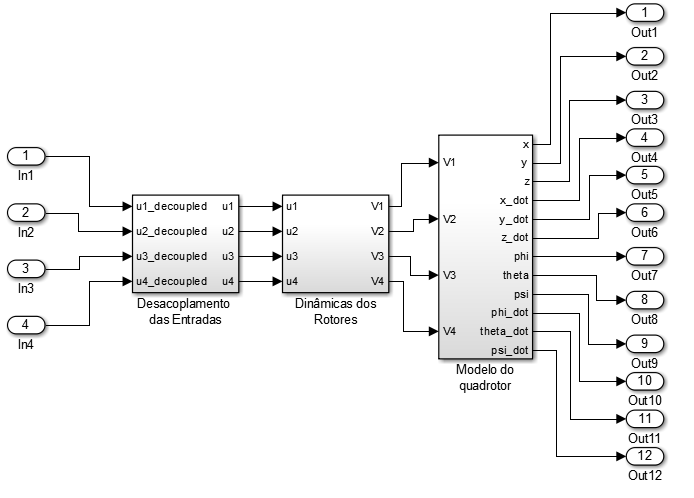
\includegraphics[width=.9\textwidth]{./04-figuras/simulink_drone/diagrama_geral}
%    \label{fig:simulink-drone-diagrama-geral}
%\end{figure}
%
%\begin{figure}[!htb]
%    \centering
%    \caption{Diagrama de blocos representando a simulação do quadrotor para  verificação efeito de sinal em degrau sobre a entrada $u_1$ nos estados afetados por ela}
%    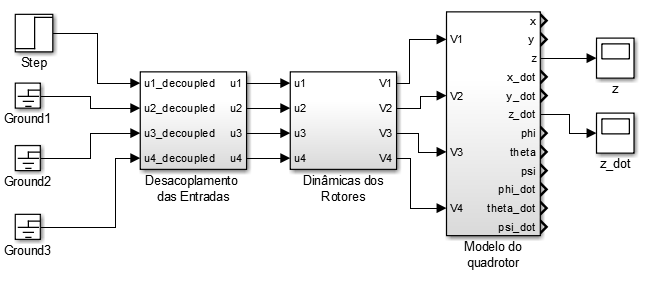
\includegraphics[width=.9\textwidth]{./04-figuras/simulink_drone/diagrama_step_u1}
%    \label{fig:simulink-drone-diagrama-step-u1}
%\end{figure}
%
%\begin{figure}[!htb]
%    \centering
%    \caption{Diagrama de blocos representando a simulação do quadrotor para  verificação efeito de sinal em degrau sobre a entrada $u_2$ nos estados afetados por ela}
%    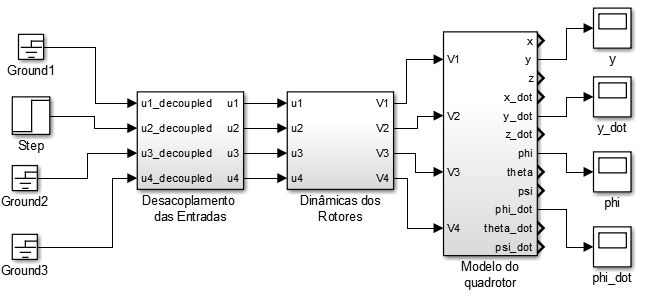
\includegraphics[width=.9\textwidth]{./04-figuras/simulink_drone/diagrama_step_u2}
%    \label{fig:simulink-drone-diagrama-step-u2}
%\end{figure}
%
%\begin{figure}[!htb]
%    \centering
%    \caption{Diagrama de blocos representando a simulação do quadrotor para  verificação efeito de sinal em degrau sobre a entrada $u_3$ nos estados afetados por ela}
%    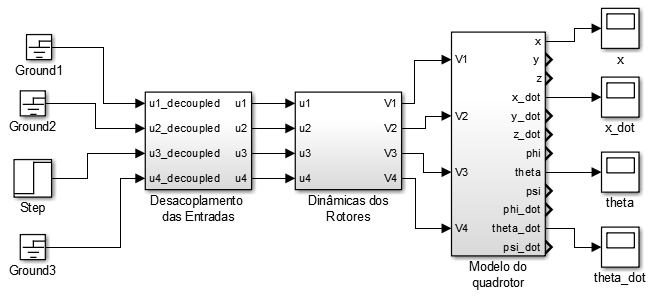
\includegraphics[width=.9\textwidth]{./04-figuras/simulink_drone/diagrama_step_u3}
%    \label{fig:simulink-drone-diagrama-step-u3}
%\end{figure}
%
%\begin{figure}[!htb]
%    \centering
%    \caption{Diagrama de blocos representando a simulação do quadrotor para  verificação efeito de sinal em degrau sobre a entrada $u_4$ nos estados afetados por ela}
%    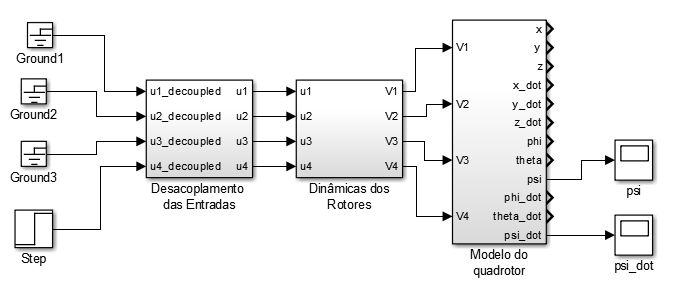
\includegraphics[width=.9\textwidth]{./04-figuras/simulink_drone/diagrama_step_u4}
%    \label{fig:simulink-drone-diagrama-step-u4}
%\end{figure}
%
%%$x$, $\dot{x}$, $\theta$ e $\dot{\theta}$
%
%Num segundo momento, é mostrada a resposta oferecida a uma entrada em degrau pelo quadrotor quando controlado por um controlador PID modelado também por \citeonline{Balas2007}. Neste momento, espera-se que o sistema não divirja e alcance a estabilidade em regime permanente. O mesmo teste é feito mas usando um controlador LQR no lugar do controlador PID. Assim como o controlador PID, o LQR também foi modelado em \citeonline{Balas2007}.
%
%Os ajustes utilizados com os ganhos utilizados na realimentação dos controladores PID e LQR são expostos nas Tabelas \ref{tab:quadrotor-controle-pid} e \ref{tab:quadrotor-controle-lqr}, respectivamente.
%
%\begin{table}[!htb]
    \centering
    \caption{Valores dos ganhos de realimentação do controlador PID projetado para o controle do quadrotor\label{tab:quadrotor-controle-pid}}
    \begin{tabular}{ccccc}
        \cline{2-5}
        & \multicolumn{4}{c}{\textbf{Variáveis controladas}} \\
        
        \hline
        \multicolumn{1}{ c }{\textbf{Variável Realimentada}} & 
                            \textbf{$x$} &
                            \textbf{$y$} & 
                            \textbf{$z$}  & 
                            \textbf{$\psi$} \\
        \hline
        \multicolumn{1}{ c }{\textbf{$\dot{\theta}$}} & 
                            5 &
                            - & 
                            - & 
                            - \\
        \hline
        \multicolumn{1}{ c }{\textbf{$\theta$}} & 
                            37,3 &
                            - & 
                            - & 
                            - \\

        \hline
        \multicolumn{1}{ c }{\textbf{$x$}} & 
                            -10,92 &
                            - & 
                            - & 
                            - \\
        \hline
        \multicolumn{1}{ c }{\textbf{$\dot{x}$}} & 
                            -10,9 &
                            - & 
                            - & 
                            - \\
        \hline
        \multicolumn{1}{ c }{\textbf{$\dot{\phi}$}} & 
                            -  &
                            5 & 
                            - & 
                            - \\
        \hline
        \multicolumn{1}{ c }{\textbf{$\phi$}} & 
                            -  &
                            37,3 & 
                            - & 
                            - \\
        \hline
        \multicolumn{1}{ c }{\textbf{$y$}} & 
                            -  &
                            10,92 & 
                            - & 
                            - \\
        \hline
        \multicolumn{1}{ c }{\textbf{$\dot{y}$}} & 
                            -  &
                            10,9 & 
                            - & 
                            - \\
        \hline
        \multicolumn{1}{ c }{\textbf{$\dot{\psi}$}} & 
                            -  &
                            - & 
                            -10 & 
                            - \\
        \hline
        \multicolumn{1}{ c }{\textbf{$\psi$}} & 
                            -  &
                            - & 
                            -10,6 & 
                            - \\
        \hline
        \multicolumn{1}{ c }{\textbf{$z$}} & 
                            - &
                            - & 
                            - & 
                            3 \\
        \hline
        \multicolumn{1}{ c }{\textbf{$\dot{z}$}} & 
                            - &
                            - & 
                            - & 
                            7,56 \\
        \hline
    \end{tabular}

    \fonte{Adaptado de \citeonline[p.~64]{Balas2007}}
\end{table}

%
%\begin{table}[!htb]
    \centering
    \caption{Valores dos ganhos de realimentação do controlador LQR projetado para o controle do quadrotor\label{tab:quadrotor-controle-lqr}}
    \begin{tabular}{ccccc}
        \cline{2-5}
        & \multicolumn{4}{c}{\textbf{Variáveis controladas}} \\
        
        \hline
        \multicolumn{1}{ c }{\textbf{Variável Realimentada}} & 
                            \textbf{$x$} &
                            \textbf{$y$} & 
                            \textbf{$z$}  & 
                            \textbf{$\psi$} \\
        \hline
        \multicolumn{1}{ c }{\textbf{$\dot{\theta}$}} & 
                            4,3043 &
                            - & 
                            - & 
                            - \\
        \hline
        \multicolumn{1}{ c }{\textbf{$\theta$}} & 
                            25,2884 &
                            - & 
                            - & 
                            - \\

        \hline
        \multicolumn{1}{ c }{\textbf{$x$}} & 
                            -7,8458 &
                            - & 
                            - & 
                            - \\
        \hline
        \multicolumn{1}{ c }{\textbf{$\dot{x}$}} & 
                            -10 &
                            - & 
                            - & 
                            - \\
        \hline
        \multicolumn{1}{ c }{\textbf{$\dot{\phi}$}} & 
                            -  &
                            4,2976 & 
                            - & 
                            - \\
        \hline
        \multicolumn{1}{ c }{\textbf{$\phi$}} & 
                            -  &
                            25,2673 & 
                            - & 
                            - \\
        \hline
        \multicolumn{1}{ c }{\textbf{$y$}} & 
                            -  &
                            7,8431 & 
                            - & 
                            - \\
        \hline
        \multicolumn{1}{ c }{\textbf{$\dot{y}$}} & 
                            -  &
                            10 & 
                            - & 
                            - \\
        \hline
        \multicolumn{1}{ c }{\textbf{$\dot{\psi}$}} & 
                            -  &
                            - & 
                            -15,7751 & 
                            - \\
        \hline
        \multicolumn{1}{ c }{\textbf{$\psi$}} & 
                            -  &
                            - & 
                            -31,6228 & 
                            - \\
        \hline
        \multicolumn{1}{ c }{\textbf{$z$}} & 
                            - &
                            - & 
                            - & 
                            3,9936 \\
        \hline
        \multicolumn{1}{ c }{\textbf{$\dot{z}$}} & 
                            - &
                            - & 
                            - & 
                            10 \\
        \hline
    \end{tabular}

    \fonte{Adaptado de \citeonline[p.~68]{Balas2007}}
\end{table}

%
%\fi

           % Metodologia
%    %
% Documento: Resultados
%
\chapter{Resultados}
\label{chap:resultados}

%Ao aplicar um impulso nas entradas do sistema modelado para representar o quadrotor, os estados relacionados à altitude e atitude divergem, como é mostrado na Figura \ref{fig:uncontrolled}. Nota-se que a divergência dos ângulos ($\phi$ e $\theta$) é linear, mostrando que o impulso aplicada na entrada é, de fato, a aceleração do sistema sobre essas saídas. Já a variável relacionada à atitude ($z$) decai em parábola, devido à ação da gravidade, o que indica que o impulso é também, de fato, uma aceleração extra do sistema no eixo $z$, como a modelagem adotada propõe.

% Sistema nao controlado
\begin{figure}[!htb]
    \centering
    \caption{Divergência das variáveis relacionadas a altitude e atitude quando o sistema é submetido a um impulso nas entradas}
    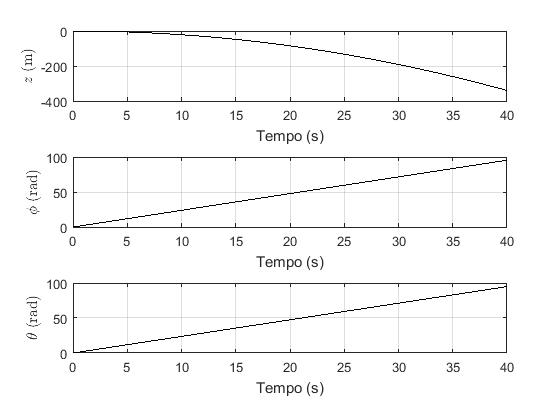
\includegraphics[width=0.8\textwidth]{./04-figuras/resultados/novos/uncontrolled}
    \label{fig:uncontrolled}
\end{figure}

Com estes resultados, fica clara a necessidade de controladores para estabilizar o sistema. Os próximos resultados mostram a resposta do sistema estabilizado pelos controladores fuzzy e neuro-fuzzy projetados.

A Figura \ref{fig:altitude_z_zdot_2kg} mostra a posição no eixo vertical ($z$) do \textit{drone}, bem como sua variação no sistema em que atua o controlador \textit{fuzzy} projetado. Como se pode ver, o distúrbio foi devidamente controlado, fazendo com que o quadricóptero retornasse à posição inicial $z=-2$ m e também ao repouso\footnote{i.e.\ velocidade nula} representado por $\dot{z}=0$ m/s. Nesta figura, entretanto, não fica tão clara a diferença de desempenho dos controladores \textit{fuzzy} e neuro-\textit{fuzzy}, aspecto que pode ser claramente verificado na Figura \ref{fig:altitude_z_zdot_2kg_closer}. Como se pode ver, tanto para $z$ quanto para $\dot{z}$, o neuro-\textit{fuzzy} apresenta desempenho melhor. No controle sobre a posição $z$, o controlador neuro-\textit{fuzzy} apresentou redução do tempo de convergência em 29\%, e da variação do sistema em 31\%, além de eliminar a sobrelevação apresentada pelo \textit{fuzzy}. Já sobre a velocidade $\dot{z}$, apresentou uma redução no tempo de convergência de 29\% além melhorar a variação do sistema em 23\%. A partir destes resultados, verifica-se que o controlador neuro-\textit{fuzzy} fez com que o distúrbio fosse melhor absorvido e que sua correção ocorresse mais rapidamente.

% Altitude m=2
\begin{figure}[!htb]
    \centering
    \caption{Comparação da resposta das saídas $z$ e $\dot{z}$ no controle de altitude \textit{fuzzy} e neuro-\textit{fuzzy} para o sistema com massa $m=2$ kg}
    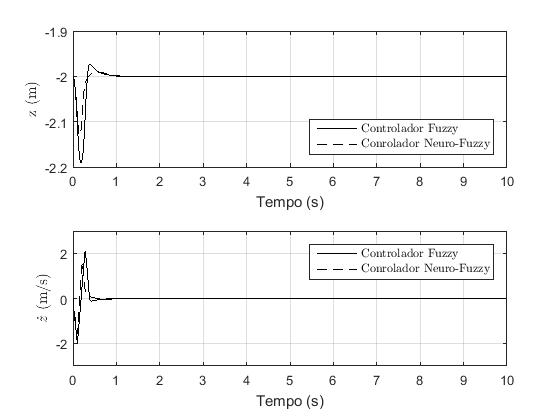
\includegraphics[width=0.8\textwidth]{./04-figuras/figuras_pos_banca/5-altitude2kg/graph_z_zdot_2kg}
    \label{fig:altitude_z_zdot_2kg}
\end{figure}

% Altitude m=2, closer
\begin{figure}[!htb]
    \centering
    \caption{Comparação em mais detalhes da resposta das saídas $z$ e $\dot{z}$ no controle de altitude fuzzy e neuro-fuzzy para o sistema com massa $m=2$ kg}
    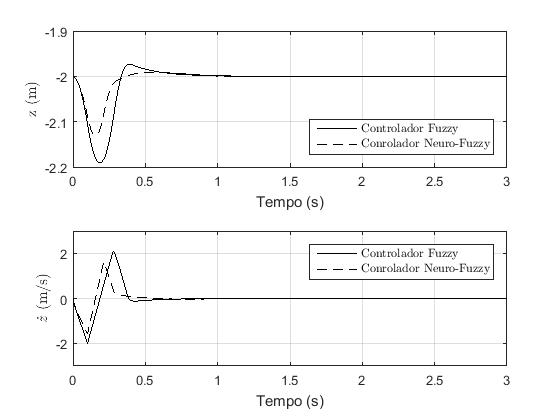
\includegraphics[width=0.8\textwidth]{./04-figuras/figuras_pos_banca/5-altitude2kg/graph_z_zdot_2kg_details}
    \label{fig:altitude_z_zdot_2kg_closer}
\end{figure}

% -------------------  ATITUDE ---------------

Já as Figuras \ref{fig:atitude_phi_phidot_2kg_40s} e \ref{fig:atitude_theta_thetadot_2kg_40s} mostram a estabilidade de atitude em torno dos eixos x e y (i.e\ em relação ao plano horizontal XY), representados por $\theta$ e $\phi$ respectivamente. Como se pode ver, ambos os estados são devidamente controlados e, com isto, o quadrotor volta à estabilidade horizontal, com ângulos e velocidades angulares nulas no estado permanente.

% Atitude m=2
%phi
\begin{figure}[!htb]
    \centering
    \caption{Comparação da resposta das saídas $\phi$ e $\dot{\phi}$ no controle de atitude fuzzy e neuro-fuzzy para o sistema com massa $m=2kg$}
    \includegraphics[width=0.8\textwidth]{./04-figuras/resultados/novos/atitude_phi_phidot_2kg_40s}
    \label{fig:atitude_phi_phidot_2kg_40s}
\end{figure}

%theta
\begin{figure}[!htb]
    \centering
    \caption{Comparação da resposta das saídas $\theta$ e $\dot{\theta}$ no controle de atitude fuzzy e neuro-fuzzy para o sistema com massa $m=2kg$}
    \includegraphics[width=0.8\textwidth]{./04-figuras/resultados/novos/atitude_theta_thetadot_2kg_40s}
    \label{fig:atitude_theta_thetadot_2kg_40s}
\end{figure}

A partir das Figuras \ref{fig:atitude_phi_phidot_2kg_10s} e \ref{fig:atitude_theta_thetadot_2kg_10s}, que mostram as respostas obtidas em mais detalhes, pode-se ver que, mais uma vez o controlador neuro-fuzzy mais uma vez teve desempenho superior ao fuzzy, fazendo com que os ângulos $\phi$ e $\theta$ convergissem 2\% mais rápido, além de reduzir suas variações em 13\%. Com relação às velocidades angulares $\dot{\phi}$ e $\dot{\theta}$, foi capaz de reduzir o tempo de convergência em 3\%, não afetando a variação nem a sobrelevação apresentada pelo sistema quando estabilizado pelo controlador fuzzy. Desta forma, verifica-se que o controle neuro-fuzzy levou o sistema a uma menor variação, representando que o ângulo máximo de inclinação alcançado pelo drone é menor e corrigido mais rapidamente.

\begin{figure}[!htb]
    \centering
    \caption{Comparação em mais detalhes da resposta das saídas $\phi$ e $\dot{\phi}$ no controle de atitude fuzzy e neuro-fuzzy para o sistema com massa $m=2kg$}
    \includegraphics[width=0.8\textwidth]{./04-figuras/resultados/novos/atitude_phi_phidot_2kg_10s}
    \label{fig:atitude_phi_phidot_2kg_10s}
\end{figure}

%theta
\begin{figure}[!htb]
    \centering
    \caption{Comparação em mais detalhes da resposta das saídas $\theta$ e $\dot{\theta}$ no controle de atitude fuzzy e neuro-fuzzy para o sistema com massa $m=2kg$}
    \includegraphics[width=0.8\textwidth]{./04-figuras/resultados/novos/atitude_theta_thetadot_2kg_10s}
    \label{fig:atitude_theta_thetadot_2kg_10s}
\end{figure}

Além da verificação da eficiência dos controladores atuando sobre o sistema para o qual foram projetados, eles foram testados num sistema em que um dos parâmetros foi acrescido de mais de 100 \%, com a massa passando de 2,3 kg para 5 kg.

A resposta dos controladores \textit{fuzzy} e neuro-\textit{fuzzy} para altitude do \textit{drone} nessas circunstâncias são mostradas nas Figuras \ref{fig:altitude_z_zdot_5kg} e \ref{fig:altitude_z_zdot_5kg_closer}, sendo que esta segunda é apenas uma forma melhor de comparar a ação dos dois controladores. Como se pode perceber, ambos os controladores levaram à estabilização do sistema, sendo que desta vez cada um obteve desempenho melhor sob determinados aspectos. No controle da posição vertical $z$, o neuro-fuzzy apresentou tempo de convergência 57\% maior, em parte causado por uma sobrelevação, que não foi apresentada pelo \textit{fuzzy}. Em contrapartida, o neuro-fuzzy apresentou uma menor variação, a reduzindo em 20\% se comparado ao \textit{fuzzy}. Com relação à velocidade $\dot{z}$, o controlador neuro-\textit{fuzzy} apresentou aumento de 23\% no tempo de convergência, mas melhorou o sistema nos quesitos variação e sobrelevação, as reduzindo em 16\% e 33\%, respectivamente. Esses resultados apontam que o quadricóptero, quando submetido ao controle neuro-\textit{fuzzy}, apresentou movimentos mais suaves até ter sua altitude estabilizada, apesar de ter sido necessário mais tempo para que ela ocorresse.

% Altitude m=5
\begin{figure}[!htb]
    \centering
    \caption{Comparação da resposta das saídas $z$ e $\dot{z}$ no controle de altitude \textit{fuzzy} e neuro-\textit{fuzzy} para o sistema com massa $m=5$ kg}
    \includegraphics[width=0.8\textwidth]{./04-figuras/resultados/novos/altitude_z_zdot_5kg}
    \label{fig:altitude_z_zdot_5kg}
\end{figure}

% Altitude m=5, closer
\begin{figure}[!htb]
    \centering
    \caption{Comparação em mais detalhes da resposta das saídas $z$ e $\dot{z}$ no controle de altitude \textit{fuzzy} e neuro-\textit{fuzzy} para o sistema com massa $m=5$ kg}
    \includegraphics[width=0.8\textwidth]{./04-figuras/resultados/novos/altitude_z_zdot_5kg_closer}
    \label{fig:altitude_z_zdot_5kg_closer}
\end{figure}


% -------------------  ATITUDE ---------------

Por fim, as Figuras \ref{fig:atitude_phi_phidot_5kg_40s} e \ref{fig:atitude_theta_thetadot_5kg_40s} mostram os resultados obtidos pelos controladores de atitude no sistema com massa $m=5$ kg. Percebe-se que mais uma vez o sistema convergiu ao seu estado de estabilidade com os ângulos nulos e velocidades angulares também nulas, representando que o quadricóptero, após a ação de controle, tanto \textit{fuzzy} quanto neuro-\textit{fuzzy}, fica estável e com orientação plana\footnote{i.e\ paralela ao plano XY}.

As Figuras \ref{fig:atitude_phi_phidot_5kg_10s} e \ref{fig:atitude_theta_thetadot_5kg_10s} mostram em mais detalhes as repostas obtidas pelos controladores sobre a atitude do sistema com massa $m=5$ kg. A partir delas, nota-se que mais uma vez o controlador neuro-\textit{fuzzy} apresentou desempenho levemente superior ao \textit{fuzzy}. Sobre os ângulos $\phi$ e $\theta$, a convergência ocorreu 3\% mais rapidamente e a variação apresentada reduziu 14\%. Já sobre as velocidades angulares $\dot{\phi}$ e $\dot{\theta}$, a redução de tempo de convergência com o neuro-\textit{fuzzy} foi de 2\%, mantendo a mesma sobrelevação e variação oferecidas pelo \textit{fuzzy}. Com isto, mais uma vez o controle neuro-fuzzy fez com que o ângulo máximo de inclinação do \textit{drone} fosse inferior ao alcançado pelo sistema controlado pelo \textit{fuzzy},e além de reduzir o tempo necessário para sua estabilização definitiva.

%phi
\begin{figure}[!htb]
    \centering
    \caption{Comparação da resposta das saídas $\phi$ e $\dot{\phi}$ no controle de atitude \textit{fuzzy} e neuro-\textit{fuzzy} para o sistema com massa $m=5$ kg}
    \includegraphics[width=0.8\textwidth]{./04-figuras/resultados/novos/atitude_phi_phidot_5kg_40s}
    \label{fig:atitude_phi_phidot_5kg_40s}
\end{figure}

%theta
\begin{figure}[!htb]
    \centering
    \caption{Comparação da resposta das saídas $\theta$ e $\dot{\theta}$ no controle de atitude \textit{fuzzy} e neuro-\textit{fuzzy} para o sistema com massa $m=5$ kg}
    \includegraphics[width=0.8\textwidth]{./04-figuras/resultados/novos/atitude_theta_thetadot_5kg_40s}
    \label{fig:atitude_theta_thetadot_5kg_40s}
\end{figure}

\begin{figure}[!htb]
    \centering
    \caption{Comparação da resposta das saídas $\phi$ e $\dot{\phi}$ no controle de atitude \textit{fuzzy} e neuro-\textit{fuzzy} para o sistema com massa $m=5$ kg}
    \includegraphics[width=0.8\textwidth]{./04-figuras/resultados/novos/atitude_phi_phidot_5kg_10s}
    \label{fig:atitude_phi_phidot_5kg_10s}
\end{figure}

%theta
\begin{figure}[!htb]
    \centering
    \caption{Comparação da resposta das saídas $\theta$ e $\dot{\theta}$ no controle de atitude \textit{fuzzy} e neuro-\textit{fuzzy} para o sistema com massa $m=5$ kg}
    \includegraphics[width=0.8\textwidth]{./04-figuras/resultados/novos/atitude_theta_thetadot_5kg_10s}
    \label{fig:atitude_theta_thetadot_5kg_10s}
\end{figure}






%\section{Resultados Obtidos na Literatura}
%\label{sec:resultados-literatura}
%
%Na literatura, diferentes controladores obtiveram diferentes resultados. 

Em \cite{Boubertakh2013}, foi proposto um controlador PID de atitude cuja resposta é mostrada nas Figuras \ref{fig:Boubertakh2013_pitch} e \ref{fig:Boubertakh2013_roll}. Como se pode ver, a orientação adotada para o ângulo de \textit{pitch}, $\theta$, é invertida em relação à adotada nesse trabalho, mas isso não prejudica a interpretação dos dados. Nota-se que, o sistema para ambos as variáveis convergiu num tempo pouco menor do que dois segundos. O valor exato para o tempo não foi especificado por \citeonline{Boubertakh2013}, mas um valor aproximado pode ser extraído a partir da análise do gráfico.

\begin{figure}[!htb]
    \centering
    \caption{Reposta do ângulo $\theta$ obtido por um controlador PID em \cite{Boubertakh2013}}
    \includegraphics[width=0.6\textwidth]{./04-figuras/resultados/comparacao_outros/18_Boubertakh2013_pitch}
    \fonte{\citeonline{Boubertakh2013}}
    \label{fig:Boubertakh2013_pitch}
\end{figure}
%
\begin{figure}[!htb]
    \centering
    \caption{Reposta do ângulo $\phi$ obtido por um controlador PID em \cite{Boubertakh2013}}
    \includegraphics[width=0.6\textwidth]{./04-figuras/resultados/comparacao_outros/18_Boubertakh2013_roll}
    \fonte{\citeonline{Boubertakh2013}}
    \label{fig:Boubertakh2013_roll}
\end{figure}





\section{Análise Consolidada dos Resultados}

Como se pode ver, os controladores de atitude e altitude tanto fuzzy quanto neuro-fuzzy foram eficientes levando à estabilização do sistema em todos os casos testados, inclusive na situação em que a massa do sistema foi aumentada em mais de 100 \%. Isso indica que estes controladores podem ser utilizados, por exemplo, em situações em que o drone precisaria transportar uma carga que tenha sua massa ou até mesmo uma superior.

Em quase todos os casos, nota-se um comportamento do controlador neuro-fuzzy superior ao do \textit{fuzzy}, o que já era esperado tendo em vista que o primeiro alia o poder do segundo às vantagens das RNAs, fazendo com que, a partir de um treinamento supervisionado utilizando o próprio modelo \textit{fuzzy}, possa se construir um controle mais abrangente e com resposta melhorada. Além disto, verificou-se uma melhora no consumo energético no controle de altitude ao utilizar o controlador neuro-\textit{fuzzy}. No controle de atitude, entretanto, o controlador neuro-\textit{fuzzy} apresentou pior eficiência energética.

Já no experimento envolvendo ruídos de medição, o controlador neuro-\textit{fuzzy} de altitude se mostrou muito superior ao \textit{fuzzy}, apresentando menor variação e menor tempo de convergência além de uma eficiência energética muito melhor, atuando de forma muito sutil para as correções dos ruídos incluídos no sistema ao passo que o \textit{fuzzy} gasta muito mais energia para fazer cada uma dessas correções.

Estes resultados mostram que, de fato, as técnicas de Inteligência Computacional podem ser aplicadas para projetar controladores eficientes e robustos para atuar sobre sistemas multivariável e que, além disto, o poder de treinamento dos ANFISs realmente é capaz de fazer com que o desempenho de controladores neuro-\textit{fuzzy} seja melhorado se comparado ao daqueles puramente \textit{fuzzy}, tanto com relação à qualidade de resposta quanto à eficiência energética.

            % Resultados
%    %
% Documento: Conclusão
%

\chapter{Conclusão}
\label{chap:conclusao}

Ao longo deste trabalho, discorreu-se sobre o crescente uso de estratégias da Inteligência Computacional para implementar controladores de sistemas não lineares. Além disto, como foi mostrado pelos experimentos realizados, o uso de controladores devidamente projetados é fundamental para fazer com que esses sistemas instáveis atuem da forma planejada e possam ser estabilizados.

No contexto deste trabalho, o sistema controlado é um quadrotor e as variáveis são referentes à sua atitude e altitude, representando portanto um controle multivariável. As alternativas propostas como controladores foram o fuzzy e o neuro-fuzzy. A opção pelo primeiro se deveu ao fato de ele permitir a modelagem a partir de variáveis e termos linguísticos além de acrescer robustez ao sistema. Já a opção pelo segundo, neuro-fuzzy, foi devido ao fato de este agregar as características de RNAs aos sistemas fuzzy, possuindo um poder de generalização e aprendizado capaz de melhorar sua performance.

De fato, os resultados mostram que o controlador neuro-fuzzy realmente obteve melhor desempenho. No controle de altitude, reduziu o tempo de convergência em 29\% e a variação do sistema em 31\% além de eliminar a sobrelevação apresentada pelo fuzzy. O controle neuro-fuzzy de atitude também apresentou melhoras, apesar de não tão significativas quanto essas: reduziu o tempo de convergência em 2\% e a variação do sistema em 13\%.

Além disto, num teste para verificar a robustez dos controladores, a massa do sistema foi acrescida em 117\%, passando de 2 kg para 5 kg. Neste novo contexto, o controlador de atitude neuro-fuzzy mais uma vez foi superior ao fuzzy, reduzindo o tempo de convergência em 3\% e da variação em 14\%. Já no controle de altitude, o único fator melhorado pelo neuro-fuzzy foi a variação do sistema, sendo reduzida em 20\%, ao passo que seu tempo de convergência cresceu 57\%, além de ter sido inserida uma sobrelevação na resposta.

Apesar das diferenças de desempenho, os controladores fuzzy e neuro-fuzzy tanto para atitude quanto para altitude do sistema foram capazes de estabilizá-lo, mesmo quando submetido a uma variação substancial de parâmetros, que foi representada pelo aumento da massa em mais de 100\%, mostrando assim a robustez intrínseca a ambos os controladores.

%tendo em vista que, em praticamente todos os casos testados, foi ele que ofereceu menor perturbação do sistema, menor sobrelevação, e melhor tempo de convergência embora ambos os controladores tenham se mostrado eficientes, estabilizando o sistema em todos os casos testados e permitindo que, após perturbações, possa-se retornar ao estado de equilíbrio, com o drone estagnado na posição horizontal, sem nenhum tipo de movimento latitudinal ou angular. Além disto mostrou-se que os controladores conferem robustez ao sistema, permitindo que mesmo para casos extremos, como foi simulado pelo aumento significativo de carga, possa-se alcançar a estabilidade.

%De fato, os resultados mostram que o controlador neuro-fuzzy realmente obteve melhor desempenho tendo em vista que, em praticamente todos os casos testados, foi ele que ofereceu menor perturbação do sistema, menor sobrelevação, e melhor tempo de convergência embora ambos os controladores tenham se mostrado eficientes, estabilizando o sistema em todos os casos testados e permitindo que, após perturbações, possa-se retornar ao estado de equilíbrio, com o drone estagnado na posição horizontal, sem nenhum tipo de movimento latitudinal ou angular. Além disto mostrou-se que os controladores conferem robustez ao sistema, permitindo que mesmo para casos extremos, como foi simulado pelo aumento significativo de carga, possa-se alcançar a estabilidade.

Desta forma, mostra-se que se podem usar técnicas de IC para controlar, de forma robusta e eficiente, sistemas não-lineares complexos e, além disso, que controladores neuro-fuzzy podem ser utilizados para melhorar o desempenho de controladores fuzzy apesar de, em algumas situações, piorar a resposta se comparado a estes.

\section{Trabalhos futuros}
\label{sec:conclusao-trabalhosFuturos}

Os resultados obtidos neste trabalho abrem espaço para  se projetarem controladores equivalentes aos construídos ao longo dele para controlar um quadrotor real, extrapolando o cenário de simulações.


%A escolha de projetar controladores neuro-fuzzy foi baseada na suposição de que, devido à sua capacidade de aprendizado e generalização, poderiam melhorar a resposta obtida pelos controladores Fuzzy. De fato, isto foi o que ocorreu em dois dos três casos observados.
%
%Todos os controladores projetados alcançaram os resultados esperados, atuando de forma a, de fato, estabilizar a atitude (variáveis $\phi$ e $\theta$) e altitude (variável $z$) do sistema. O uso do controlador Neuro-Fuzzy sobre a variável $\phi$ aumentou a sobrelevação em quase quatro vezes apesar de não ter afetado de forma considerável no tempo de assentamento. Já sobre as variáveis $\theta$ e $z$, o controlador Neuro-Fuzzy apresentou uma ligeira redução na sobrelevação do sistema e também no tempo de assentamento.
%
%Estes resultados indicam que as características apresentadas pelos controladores Neuro-Fuzzy podem realmente melhorar o desempenho de sistemas que possuem controladores Fuzzy. Entretanto, os resultados também mostram que esta melhora não é observada em todos os casos e que um controlador Neuro-Fuzzy pode também levar à piora num controle.
             % Conclusão
    
    
	%%
% Documento: Conclusão
%

\chapter{Considerações Finais}
\label{chap:consideracoes-finais}

Este trabalho é a primeira parte do Trabalho de Conclusão de Curso.

\section{Trabalhos futuros}
\label{sec:consideracoes-finais-trabalhos-futuros}

A partir dos resultados e da conclusão, poder-se-á propor diferentes trabalhos futuros relacionados a este. Isto deverá ser feito nesta seção.
  % Considerações Finais
%\chapter{Introdução} \label{chap:introducao}
%\chapter{Fundamentação Teórica}
%\chapter{Trabalhos Relacionados}
%\chapter{Metodologia}
%\chapter{Resultados}
%\chapter{Conclusão}
%\chapter{Considerações Finais}
    % Elementos pós textuais
    \postextual
    %
% Documento: Referências Bibliográficas
%

\bibliography{./refbase}    % Geração automática das referências por meio do arquivo 'refbase.bib'
       % Referências
    %
% Documento: Apêndices
%

\begin{apendicesenv}
\partapendices

\chapter{Código para Criação de Modelo Neuro-Fuzzy para Altitude e Definição de Dados para Treinamento}
\label{chap:train-anfis-altitude}

%\lstinputlisting{03-elementos-pos-textuais/script_testing_anfis_altitude.m}
\begin{lstlisting}[inputencoding=latin1]
	% le arquivo fis referente ao controle de altitude
	fismat = readfis('fis_altitude.fis');
	
	% define numero de casos a serem avaliados (treinamento + teste)
	n = 300;
	% define conjunto de n entradas aleatorias para o sistema fuzzy
	% respeitando o range de cada entrada
	input = zeros(n,2);
	for i=1:n    
	    z_value = rand * 2 - 1;
	    z_dot_value = rand * 10 - 5;
	    input(i,:) = [ z_value z_dot_value ];
	end
	
	% avalia resposta fuzzy para cada entrada
	output= evalfis(input,fismat);
	
	% define data como vetor relacionando cada conjunto de entradas a saida
	% - obtida pelo sistema fuzzy
	data = [];
	for i=1:n
	   data(i,:) = [ input(i,:) output(i) ];
	end
	
	% define que 2/3 dos dados obtidos serao usasdos para treinamento
	% e 1/3 sera usado para teste da rede
	train = data(1:2*n/3,:);    % dados para treinamento
	test = data(2*n/3+1:n,:);   % dados para validacao do sistema treinado
	
	% gera modelo fuzzy Sugeno a partir do Mamdani modelado
	sugFIS = mam2sug(fismat);
	% salva modelo Sugeno em disco com o nome fis_altitude_neuro.fis
	writefis(sugFIS, 'fis_altitude_neuro.fis');
\end{lstlisting}


\chapter{Código para Criação de Modelo Neuro-Fuzzy para Atitude e Definição de Dados para Treinamento}
\label{chap:train-anfis-atitude}

\begin{lstlisting}[inputencoding=latin1]
	% le arquivo fis referente ao controle de atitude
	fismat = readfis('fis_atitude.fis'); 
	
	% define numero de casos a serem avaliados (treinamento + teste)
	n = 300;
	% define conjunto de n entradas aleatorias para o sistema fuzzy
	% respeitando o range de cada entrada
	input = zeros(n,2);
	for i=1:n
	    phi_value = rand * 4 - 2;
	    phi_dot_value = rand * 3 - 1.5;
	    input(i,:) = [ phi_value phi_dot_value ];
	end
	
	% avalia resposta fuzzy para cada entrada
	output= evalfis(input,fismat);
	
	% define data como vetor relacionando cada conjunto de entradas a saída
	% obtida pelo sistema fuzzy
	data = [];
	for i=1:n
	   data(i,:) = [ input(i,:) output(i) ];
	end
	
	% define que 2/3 dos dados obtidos serao usasdos para treinamento
	% e 1/3 sera usado para teste da rede
	train = data(1:2*n/3,:);    % dados para treinamento
	test = data(2*n/3+1:n,:);   % dados para validação do sistema treinado
	
	% gera modelo fuzzy Sugeno a partir do Mamdani modelado
	sugFIS = mam2sug(fismat);
	% salva modelo Sugeno em disco com o nome fis_atitude_neuro.fis
	writefis(sugFIS, 'fis_atitude_neuro.fis');
\end{lstlisting}

\end{apendicesenv}
         % Apêndices
    %%
% Documento: Anexos
%

\begin{anexosenv}
\partanexos

\chapter{Nome do Anexo}
\label{chap:anexox}

Inserir seu texto aqui...

\chapter{Nome do Anexo}
\label{chap:anexoy}

Inserir seu texto aqui...

\end{anexosenv}
            % Anexos
    \printindex                                             % Índice remissivo

\end{document}
